\documentclass[12pt]{article}
\usepackage{graphicx}
\usepackage{amsmath}
\usepackage{subcaption}
\usepackage{multirow}
\usepackage{float}
\usepackage{setspace}
\usepackage{enumitem}
\usepackage[utf8]{inputenc}
\usepackage[english]{babel}
\usepackage{listings}
\usepackage{geometry}
\geometry{
	a4paper,
	total={170mm,257mm},
	left=20mm,
	top=20mm,
}
\usepackage{xcolor}
\definecolor{aqua}{rgb}{0.0, 1.0, 1.0}
\definecolor{brightgreen}{rgb}{0.4, 1.0, 0.0}
\definecolor{darkblue}{rgb}{0.0, 0.0, 0.55}

\usepackage{xparse}% http://ctan.org/pkg/xparse
\NewDocumentCommand{\ceil}{s O{} m}{%
	\IfBooleanTF{#1} % starred
	{\left\lceil#3\right\rceil} % \ceil*[..]{..}
	{#2\lceil#3#2\rceil} % \ceil[..]{..}
}

\title{ \color{darkblue}  \textbf{EE338 : Digital Signal Processing \\
Filter Design Assignment}}
\author{ Garaga V V S Krishna Vamsi\\
180070020}


\begin{document}
	\pagenumbering{gobble}
	\doublespacing
	\maketitle
	\begin{center}
		Filter Number : 33\\
		Group No .2\\
		Shubham Kar 180070058\\
		Rishav Ranjan 180070045\\
	\end{center}
	
	
	\newpage	
	\color{darkblue}\tableofcontents
	\newpage
	\pagenumbering{arabic}
	\singlespacing
	\color{darkblue}
	\section{Student Details:}
	\color{black}
	\color{darkblue}\textbf{Name}\color{black}: Garaga V V S Krishna Vamsi\\
	\color{darkblue}\textbf{Roll No}\color{black}: 180070020\\
	\color{darkblue}\textbf{Filter No}\color{black}: 33\\
	\color{darkblue}\textbf{Group No}\color{black}: 2\\
	\color{darkblue}\textbf{Group Members}\color{black}:\\
	1) Shubham Kar 180070058\\
	2) Rishav Ranjan 180070045
	
	\color{darkblue}
	\section{Filter 1: Butterworth Band Pass Filter}
	\color{black}
	\begin{itemize}
		\item Filter Number Assigned = m = 33
		\item Both Pass band and Stop band tolerances are 0.15
		\item Pass band: Monotonic  (as 1 $\le$ m $\le$ 80)
		\item Stop band: Monotonic
		\item Butterworth Approximation
		\item Band-Pass filter.
		\item The Transition band is 4kHz on either side of the pass band
		\item The input signal is Band limitted to 160kHz and the sampling rate is 330kHz.
	\end{itemize}
	\color{cyan}
	\subsection{Unnormalized Specifications}
	\color{black}
	m = 33\\
	q(m) = 3\\
	r(m) = 33 - 30 = 3\\
	BL(m) = 25 + 1.7 $\times$ 3 + 6.1 $\times$ 3 = 48.4 kHz\\
	BH(m) = BL(m) + 20 = 68.4 kHz\\
	
	\noindent Hence the filter specifications for the Bandpass Filter are:
	\begin{itemize}
		\item Pass band is 48.4 kHz to 68.4 kHz
		\item Transition band is 4kHz on either side of the Pass band
		\item Stop band is 0 to 44.4 kHz and 72.4 kHz to 165 kHz
		\item Tolerances for both bands are 0.15
		\item Both Pass band and Stop band are monotonic
	\end{itemize}
	
	\color{cyan}
	\subsection{Normalized specifications}
	\color{black}
	Given sampling rate  = 330 kHz. Using\\
	\begin{gather*}
		\omega = \frac{2\pi \ast \Omega}{\Omega_s}
	\end{gather*}
	where $\omega$ is the normalized frequency, $\Omega$ is the Un-normalized frequency and $\Omega_s$ is the sampling frequency.
	\begin{itemize}
		\item Pass band is $\frac{22}{75}\pi$ to $\frac{114}{275}\pi$ $\sim$ (0.29$\pi$ to 0.415$\pi$)
		\item Transition band is $\frac{4}{165}\pi$ $\sim$ (0.024$\pi$) on either side of the Pass band
		\item Stop band is 0 to  $\frac{74}{275}\pi$ and $\frac{362}{825}\pi$ to $\pi$  $\sim$(0 to 0.27$\pi$ and  0.44$\pi$ to $\pi$)
		\item Tolerances for both bands are 0.15
		\item Both Pass band and Stop band are monotonic
	\end{itemize}
	
	\color{cyan}
	\subsection{Analog Band-pass Filter Specifications}
	\color{black}
	Using Bilinear Transformation,
	\begin{gather*}
		\Omega = tan\left(\frac{\omega}{2}\right)
	\end{gather*}
	where $\Omega$ is the analog domain frequency and $\omega$ is the discrete domain frequency\\
	
	\begin{center}
	\begin{tabular}{ |c|c|c|c|c|c|c| }
		\hline
		&&&&&&\\
		Domain& Zero & $\Omega_{S1}$ & $\Omega_{P1}$ &$\Omega_{P2}$& $\Omega_{S2}$&Infinity\\
		&&&&&&\\
		\hline
		&&&&&&\\
		$\omega$ & 0 & $\frac{74}{275}\pi$ & $\frac{22}{75}\pi$& $\frac{114}{275}\pi$& $\frac{362}{825}\pi$& $\pi$\\
		&&&&&&\\
		\hline
		&&&&&&\\
		$\Omega$ & 0 & 0.45 & 0.496 & 0.762& 0.824 & $\infty$\\
		&&&&&&\\
		\hline
	\end{tabular}
	\end{center}
	
	\noindent Hence the filter specifications for the corresponding analog domain Bandpass Filter are:
	\begin{itemize}
		\item Pass band is 0.496 ($\Omega_{P1}$)  to 0.762 ($\Omega_{P2}$) 
		\item Stop band is 0 to 0.45($\Omega_{S1}$) and 0.824 ($\Omega_{S2}$) to $\infty$
		\item Tolerances for both bands are 0.15
		\item Both Pass band and Stop band are monotonic (as 1 $\le$ m $\le$ 80)
	\end{itemize}
	
	\color{cyan}
	\subsection{Frequency Transformation in to a Low Pass Filter}
	\color{black}
	Using the Band-Pass Transformation
	\begin{gather*}
		\Omega_L = \frac{\Omega^2 - \Omega_0^2}{B\Omega}\\\\
		\Omega_0 = \sqrt{\Omega_{P1} \Omega_{P2}} = 0.615\\\\
		B = \Omega_{P2} - \Omega_{P1} = 0.2656
	\end{gather*}

	\begin{center}
		\begin{tabular}{ |c|c|c|c|c|c|c|c| }
			\hline
			&&&&&&&\\
			Domain &Zero & $\Omega_{S1}$ & $\Omega_{P1}$ &$\Omega_0$ &$\Omega_{P2}$& $\Omega_{S2}$ &Infinity\\
			&&&&&&&\\
			\hline
			&&&&&&&\\
			$\Omega$ & 0$^+$ & 0.45 & 0.496 &0.615 &0.762& 0.824 & $\infty$\\
			&&&&&&&\\
			\hline
			&&&&&&&\\
			$\Omega_L$ & -$\infty$ & -1.4727 & -1 & 0 &1 & 1.3741 & $\infty$\\
			&&&&&&&\\
			\hline
			&&&&&&&\\
			Domain& -Infinity & $\Omega_{LS1}$ & $\Omega_{LP1}$ &$\Omega_0$ &$\Omega_{LP2}$& $\Omega_{LS2}$ &Infinity\\
			&&&&&&&\\
			\hline
		\end{tabular}
	\end{center}


	\color{cyan}
	\subsection{Analog Low Pass Filter Specification}
	\color{black}
	Hence the Frequency Transformed Low-Pass Filter Specifications are:
	\begin{itemize}
		\item Pass band edge is at 1 ($\Omega_{LP}$)
		\item Stop band edge = min (-$\Omega_{LS1}$, $\Omega_{LS2}$) = 1.3741 ($\Omega_{LS}$)
		\item Tolerances = 0.15 for both Stop band and Pass band
		\item Both Pass band and Stop band are monotonic
	\end{itemize}


	\color{cyan}
	\subsection{Analog Low Pass Transfer function}
	\color{black}
	Using, Butterworth Approximation, As Tolerances of both Pass Band and Stop Band are 0.15.
	\begin{gather*}
		D_1 = \frac{1}{(1-\delta_1)^2} - 1 = 0.384\\
		D_2 = \frac{1}{\delta_2^2} - 1 = 43.44
	\end{gather*}
	\begin{gather*}
		H_{analog,LPF}^2(j\Omega) = \frac{1}{1+(\frac{\Omega}{\Omega_{c}})^{2N}} 
	\end{gather*}
	Using the inequality for Order N of the Butterworth approximation,
	\begin{gather*}
		N_{min} = \ceil[\Bigg]{ \frac{log\left(\sqrt{\frac{D2}{D1}}\right)}{log\left(\frac{\Omega_{LS}}{\Omega_{LP}}\right)}} \\
		N_{min} = 8
	\end{gather*}
	

	\noindent The Cut-off Frequency should follow the constraint:
	\begin{gather*}
		\frac{\Omega_{LP}}{(D1)^{\frac{1}{2N}}} \le \Omega_C \le \frac{\Omega_{LS}}{(D2)^{\frac{1}{2N}}} \\	
		1.0616 \le \Omega_C \le 1.0856
	\end{gather*}
	Thus we can choose $\Omega_C$ as 1.07.\\
	Now, Poles and transfer function can be obtained by solving the equation:
	\begin{gather*}
		1 + \left(\frac{s}{j\Omega_c}\right)^{2N} = 1 + \left(\frac{s}{j1.07}\right)^{16} = 0
	\end{gather*} 
	Using Wolfram to plot these poles,
	\begin{figure}[H]
		\centering
		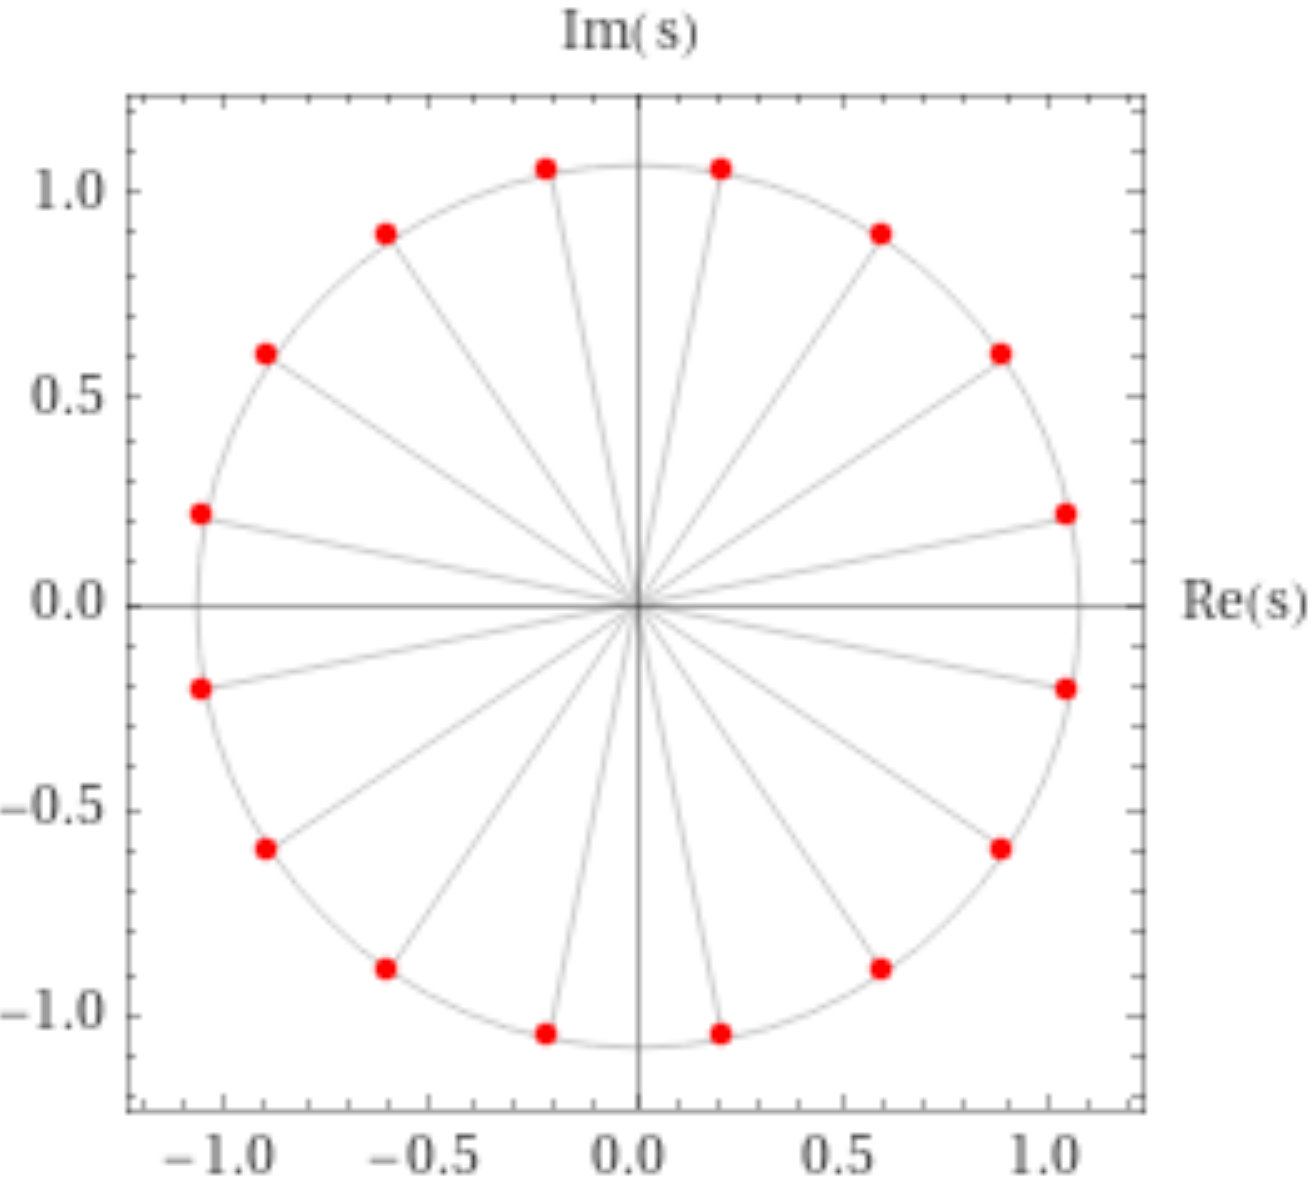
\includegraphics[width = 5cm]{Butterworthpoles.png}
	\end{figure}
	\noindent Note we need to only select those poles where the Re(s) $<$ 0 i.e only the left half plane as we want realizable specifications thus we want stability and causality
	\begin{verbatim*}	
		p1=-0.20875+1.0494i
		p2=-0.59446+0.88967i
		p3=-0.88967+0.59446i
		p4=-1.0494+0.20875i
		p5=-1.0494-0.20875i
		p6=-0.88967-0.59446i
		p7=-0.59446-0.88967i
		p8=-0.20875-1.0494i
	\end{verbatim*}
	
	\noindent Using the above 8 poles, the transfer function of this Analog Low pass filter can be written as:
	\begin{gather*}
		H_{analog, LPF}(s_L) = \frac{\Omega_C^8}{(s_L - p_1)(s_L - p_2)(s_L - p_3)(s_L - p_4)(s_L - p_5)(s_L - p_6)(s_L - p_7)(s_L - p_8)}
	\end{gather*}
	\begin{gather*}
		= \frac{1.7182}{s_L^8 + 5.4846s_L^7 + 15.0406s_L^6 + 26.7625s_L^5 + 33.672s_L^4 + 30.46s_L^3 + 19.715s_L^2 + 8.231s_L + 1.7182}
	\end{gather*}
	\begin{figure}[H]
		\centering 
		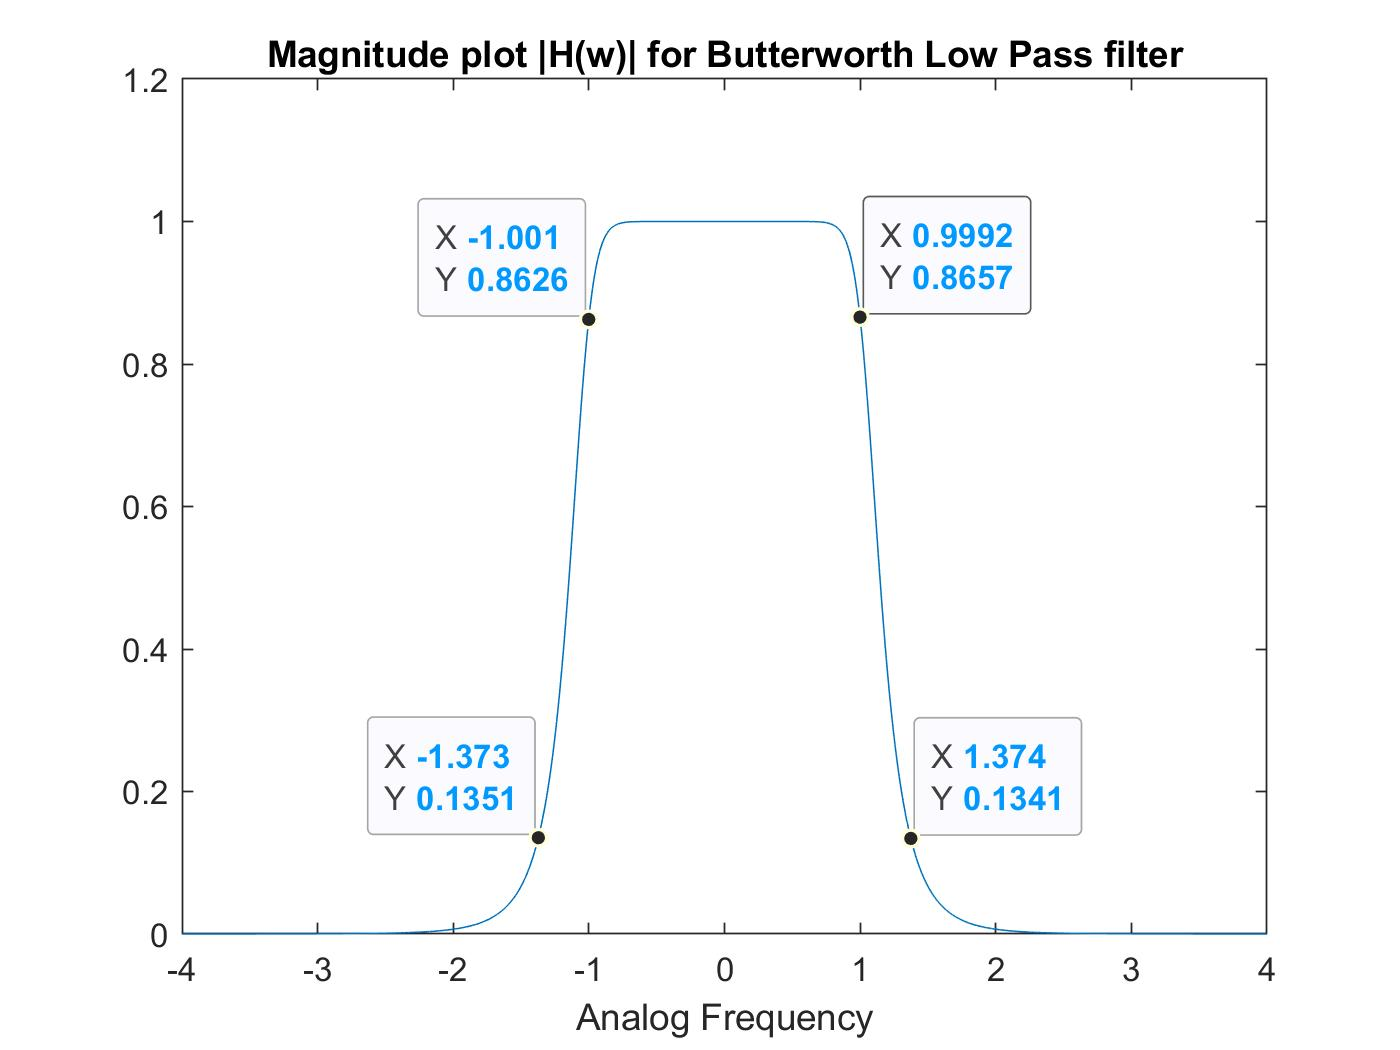
\includegraphics[width = 12cm]{Filter1ALPF.jpg}
	\end{figure}
	
	
	\color{cyan}
	\subsection{Analog Band Pass Transfer function}
	\color{black}
	
	Using the Band pass transformation:
	\begin{gather*}
		s_L = \frac{s^2 + \Omega_0^2}{Bs}
	\end{gather*}
	Substituting the values for B = 0.266 and $\Omega_0$ = 0.615,
		\begin{gather*}
		s_L = \frac{s^2 + 0.378}{0.266s}
	\end{gather*}
	
	\noindent Substituting this back into $H_{analog,LPF}(s_L)$, we get $H_{analog,BPF}(s)$. It can be written in the form N(s)/D(s) where the polynomial N(s) = 4.2604$\times$$10^{-5} s^{8}$ and the coefficients of the polynomial D(s) are:
	\begin{table}[H]
			\begin{center}
			\begin{tabular}{ |c|c|c|c|c|c|c| } 
				\hline
				Degree & $s^{16}$ & $s^{15}$ & $s^{14}$ & $s^{13}$&$s^{12}$ & $s^{11}$\\ 
				\hline
				Coefficient & 1 & 1.4570 & 4.0876 & 4.3597 & 6.5834 & 5.3676 \\
				\hline
			\end{tabular}
		\end{center}
		\begin{center}
			\begin{tabular}{ |c|c|c|c|c|c|c| } 
				\hline
				Degree & $s^{10}$ & $s^{9}$ & $s^{8}$ & $s^{7}$ & $s^{6}$& $s^{5}$\\ 
				\hline
				Coefficient & 5.5702 & 3.525 & 2.7317 & 1.3334 & 0.7971 &	0.2906\\
				\hline
			\end{tabular}
		\end{center}
		\begin{center}
			\begin{tabular}{|c|c|c|c|c|c|} 
				\hline
				Degree  & $s^{4}$ & $s^{3}$ & $s^{2}$& $s^{1}$&1\\ 
				\hline
				Coefficient & 0.1348 & 0.0338 & 0.0120 & 0.0016 & 0.00042\\
				\hline
			\end{tabular}
		\end{center}
		\caption{Coefficients of D(s)}
		\label{Table 1: }	

	\end{table}
	
	\begin{figure}[H]
		\centering
		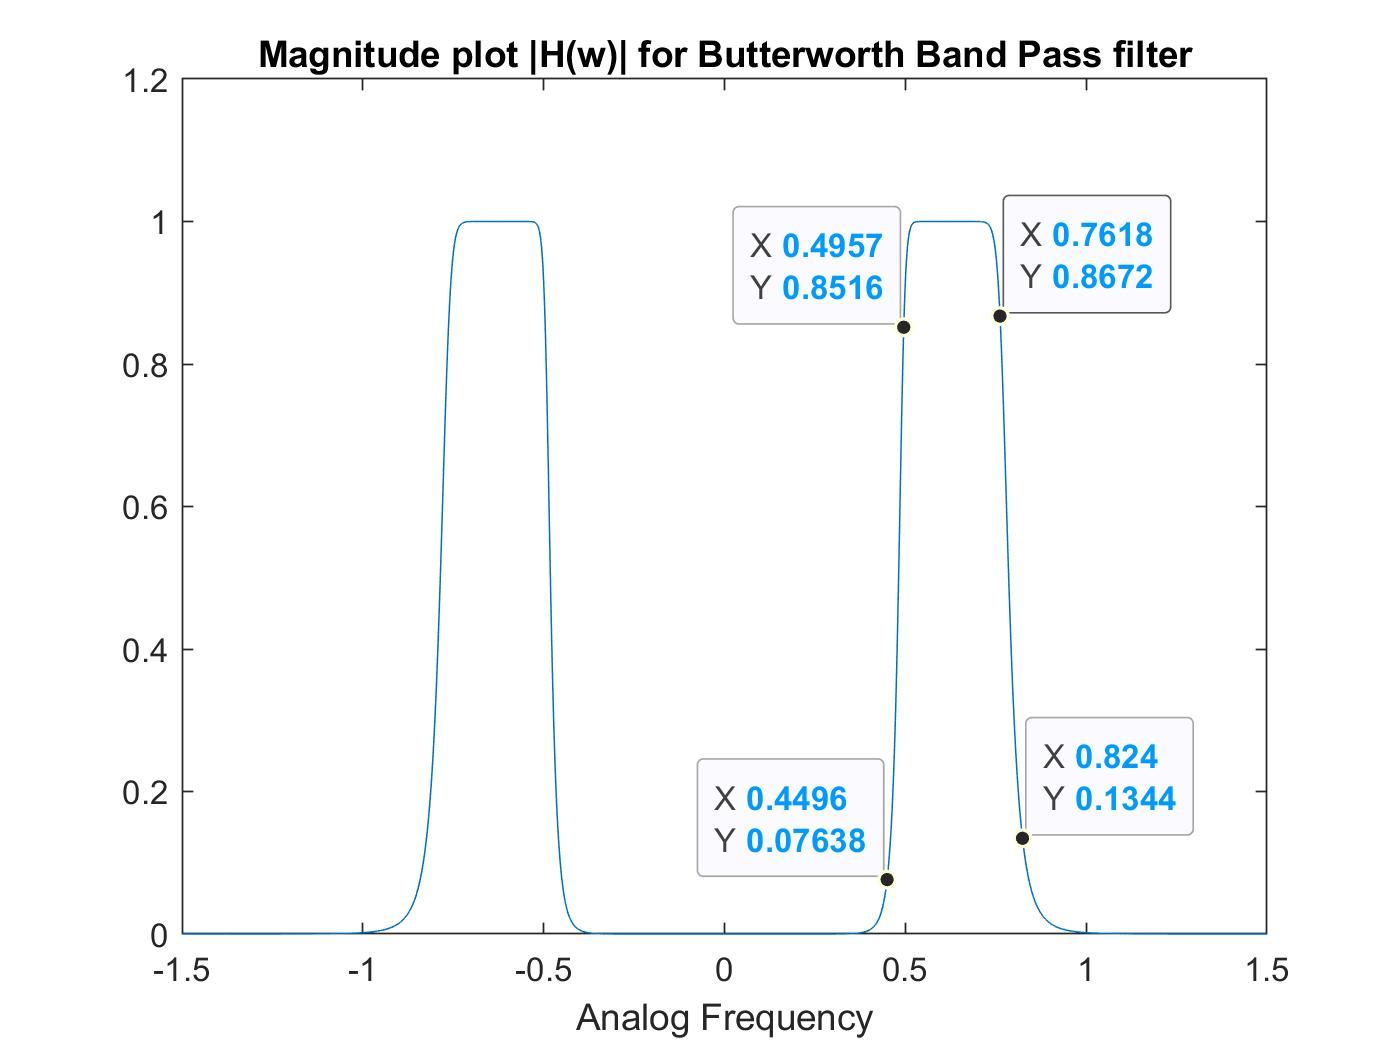
\includegraphics[width = 12cm]{Filter1ABPF.jpg}
	\end{figure}

	\color{cyan}
	\subsection{Discrete time Band Pass Transfer function}
	\color{black}
	Using the Bilinear Transformation:
	\begin{gather*}
		s = \frac{1-z^{-1}}{1+z^{-1}}
	\end{gather*}
	
	\noindent Substituting this back in $H_{Analog,BPF}(s)$, we get $H_{digital,BPF}(z)$. It can be written in the form N(z)/D(z) where the coefficients of the polynomials N(z) and D(z) are shown in the below tables. \\Coefficients of N(z) for odd powers of $z^{-1}$ are zero. 
	
	\begin{table}[H]
		\begin{center}
			\begin{tabular}{ |c|c|c|c|c|c| } 
				\hline
				Degree & 1 & $z^{-2}$ & $z^{-4}$ & $z^{-6}$&$z^{-8}$\\ 
				\hline
				Coefficient & 1.1426$\times10^{-6}$ & -9.141$\times10^{-6}$ & 3.1994$\times10^{-5}$ & -6.3897$\times10^{-5}$ & 7.9984$\times10^{-5}$\\
				\hline
			\end{tabular}
		\end{center}
		\begin{center}
			\begin{tabular}{ |c|c|c|c|c| } 
				\hline
				Degree & $z^{-10}$ & $z^{-12}$ & $z^{-14}$&$z^{-16}$\\ 
				\hline
				Coefficient & -6.3897$\times10^{-5}$  &3.1994$\times10^{-5}$ & -9.141$\times10^{-6}$ &  1.1426$\times10^{-6}$ \\
				\hline
			\end{tabular}
		\end{center}
		
		\caption{Coefficients of N(z)}
		\label{Table 2: }	
		
	\end{table}
	\begin{table}[H]
		\begin{center}
			\begin{tabular}{ |c|c|c|c|c|c|c| } 
				\hline
				Degree & 1 & $z^{-1}$ & $z^{-2}$ & $z^{-3}$&$z^{-4}$ & $z^{-5}$\\ 
				\hline
				Coefficient & 1 & -6.2775 & 23.2001 & -59.9462 & 120.0295 & -193.4666 \\
				\hline
			\end{tabular}
		\end{center}
		\begin{center}
			\begin{tabular}{ |c|c|c|c|c|c| } 
				\hline
				Degree & $z^{-6}$ & $z^{-7}$ & $z^{-8}$ & $z^{-9}$ & $z^{-10}$\\ 
				\hline
				Coefficient  & -290.3236 & 276.4138 & -223.3277 & 153.027 & -88.019\\
				\hline
			\end{tabular}
		\end{center}
		\begin{center}
			\begin{tabular}{|c|c|c|c|c|c|c|} 
				\hline
				Degree & $z^{-11}$ & $z^{-12}$ & $z^{-13}$ & $z^{-14}$& $z^{-15}$&$z^{-16}$\\ 
				\hline
				Coefficient & 258.6412 & 41.9788 & -16.1093 & 4.7895 & -0.9951 & 0.122\\
				\hline
			\end{tabular}
		\end{center}
		\caption{Coefficients of D(z)}
		\label{Table 3: }	
		
	\end{table}
	\begin{figure}[H]
		\centering
		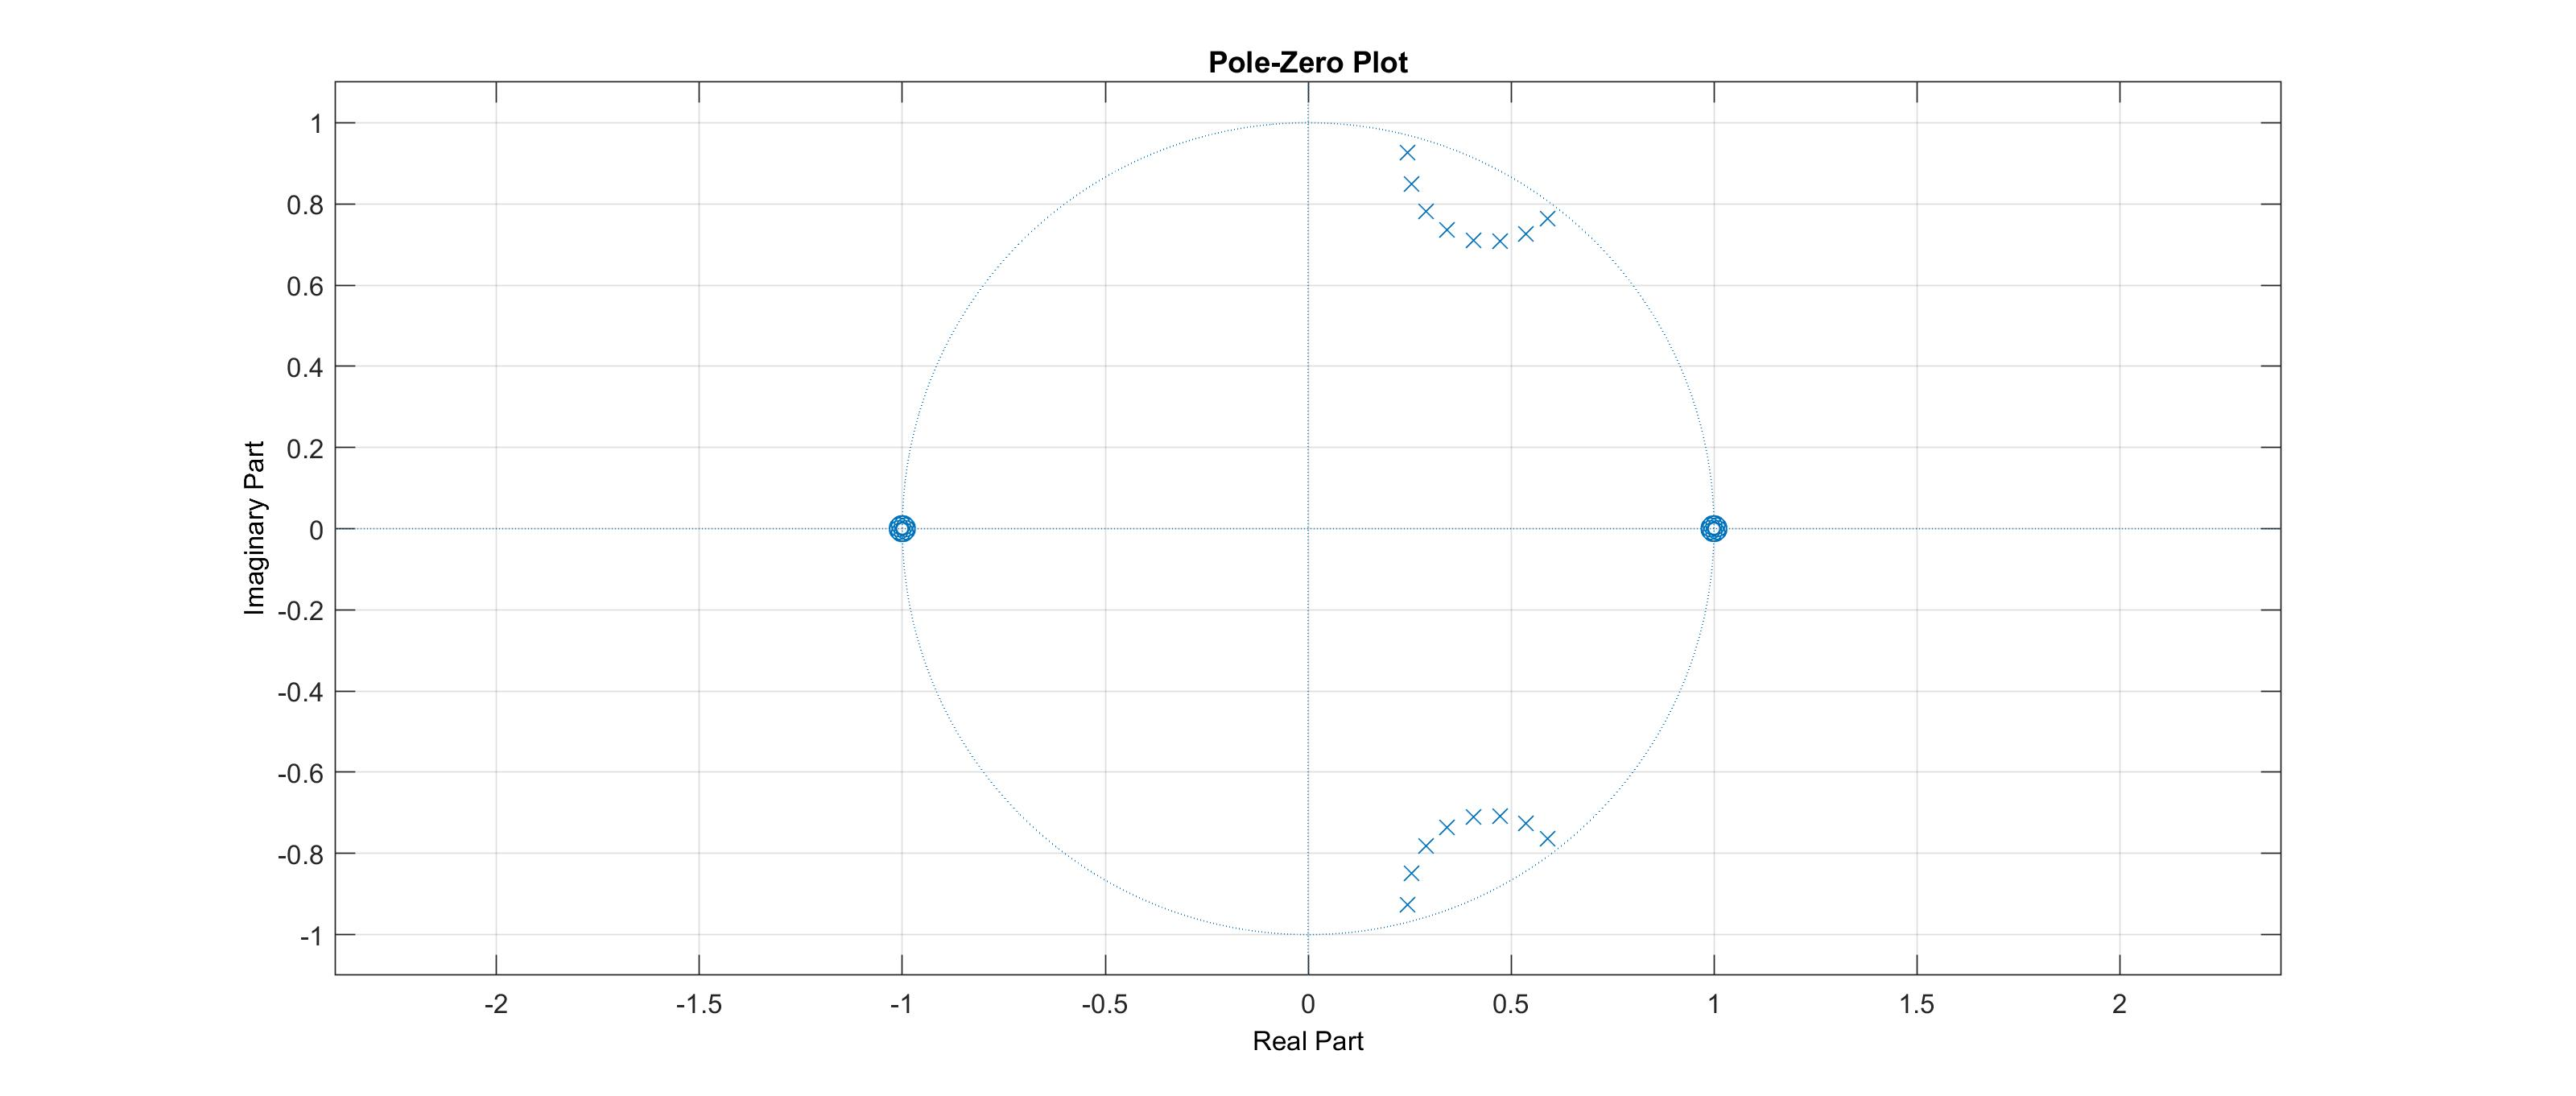
\includegraphics[width = 16cm]{Filter1PZ.jpg}
	\end{figure}

	\begin{figure}[H]
		\centering
		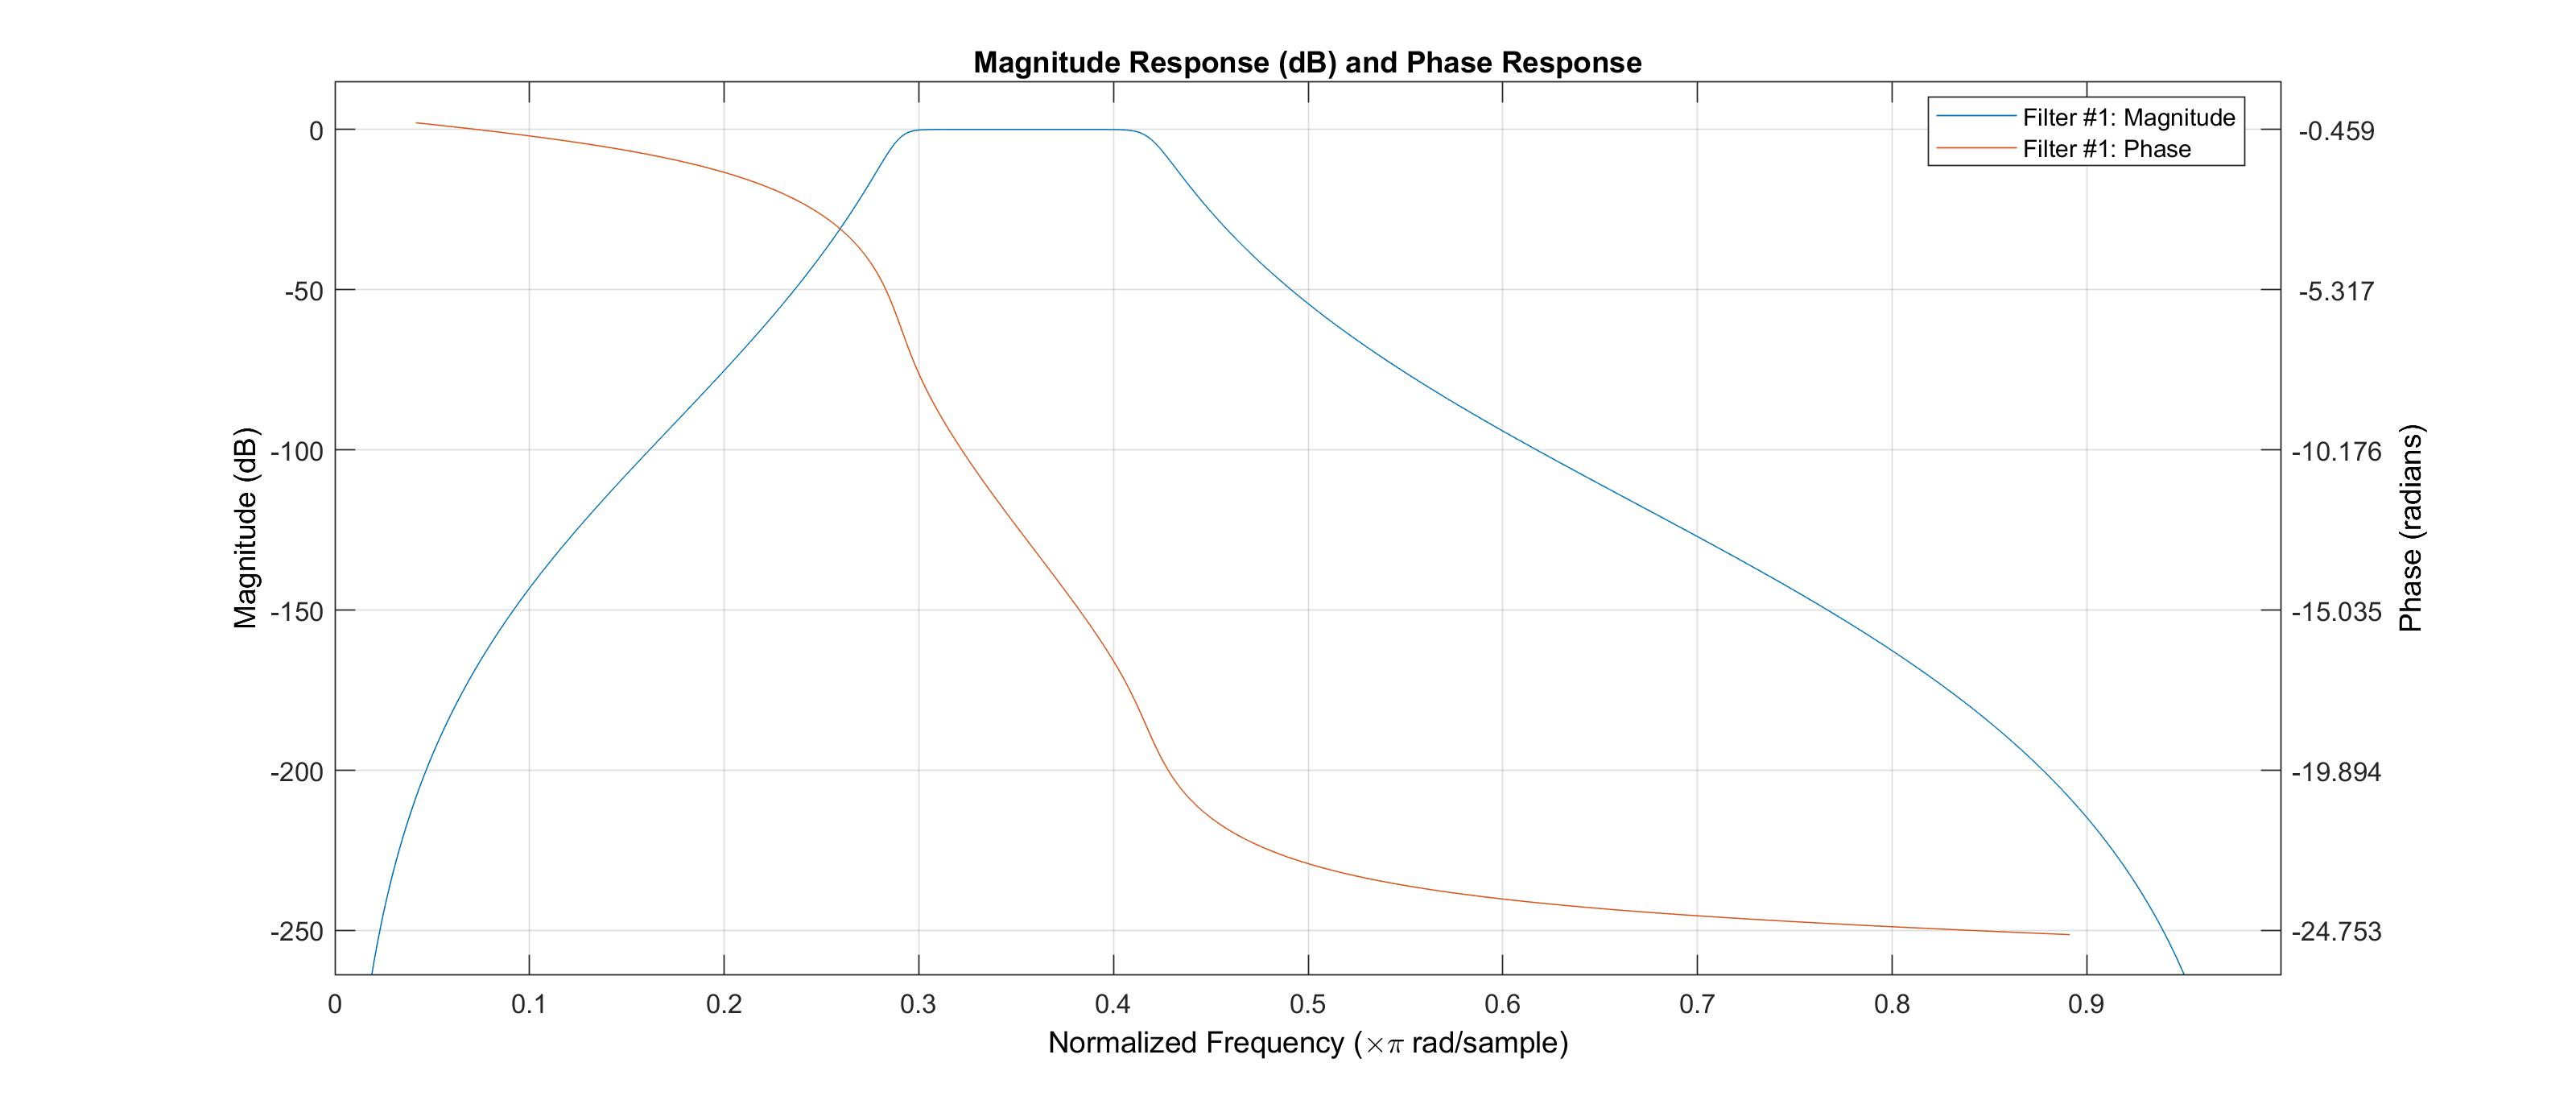
\includegraphics[width = 16cm, height = 10cm]{Filter1MagPhase.jpg}
	\end{figure}
	\begin{figure}[H]
		\centering
		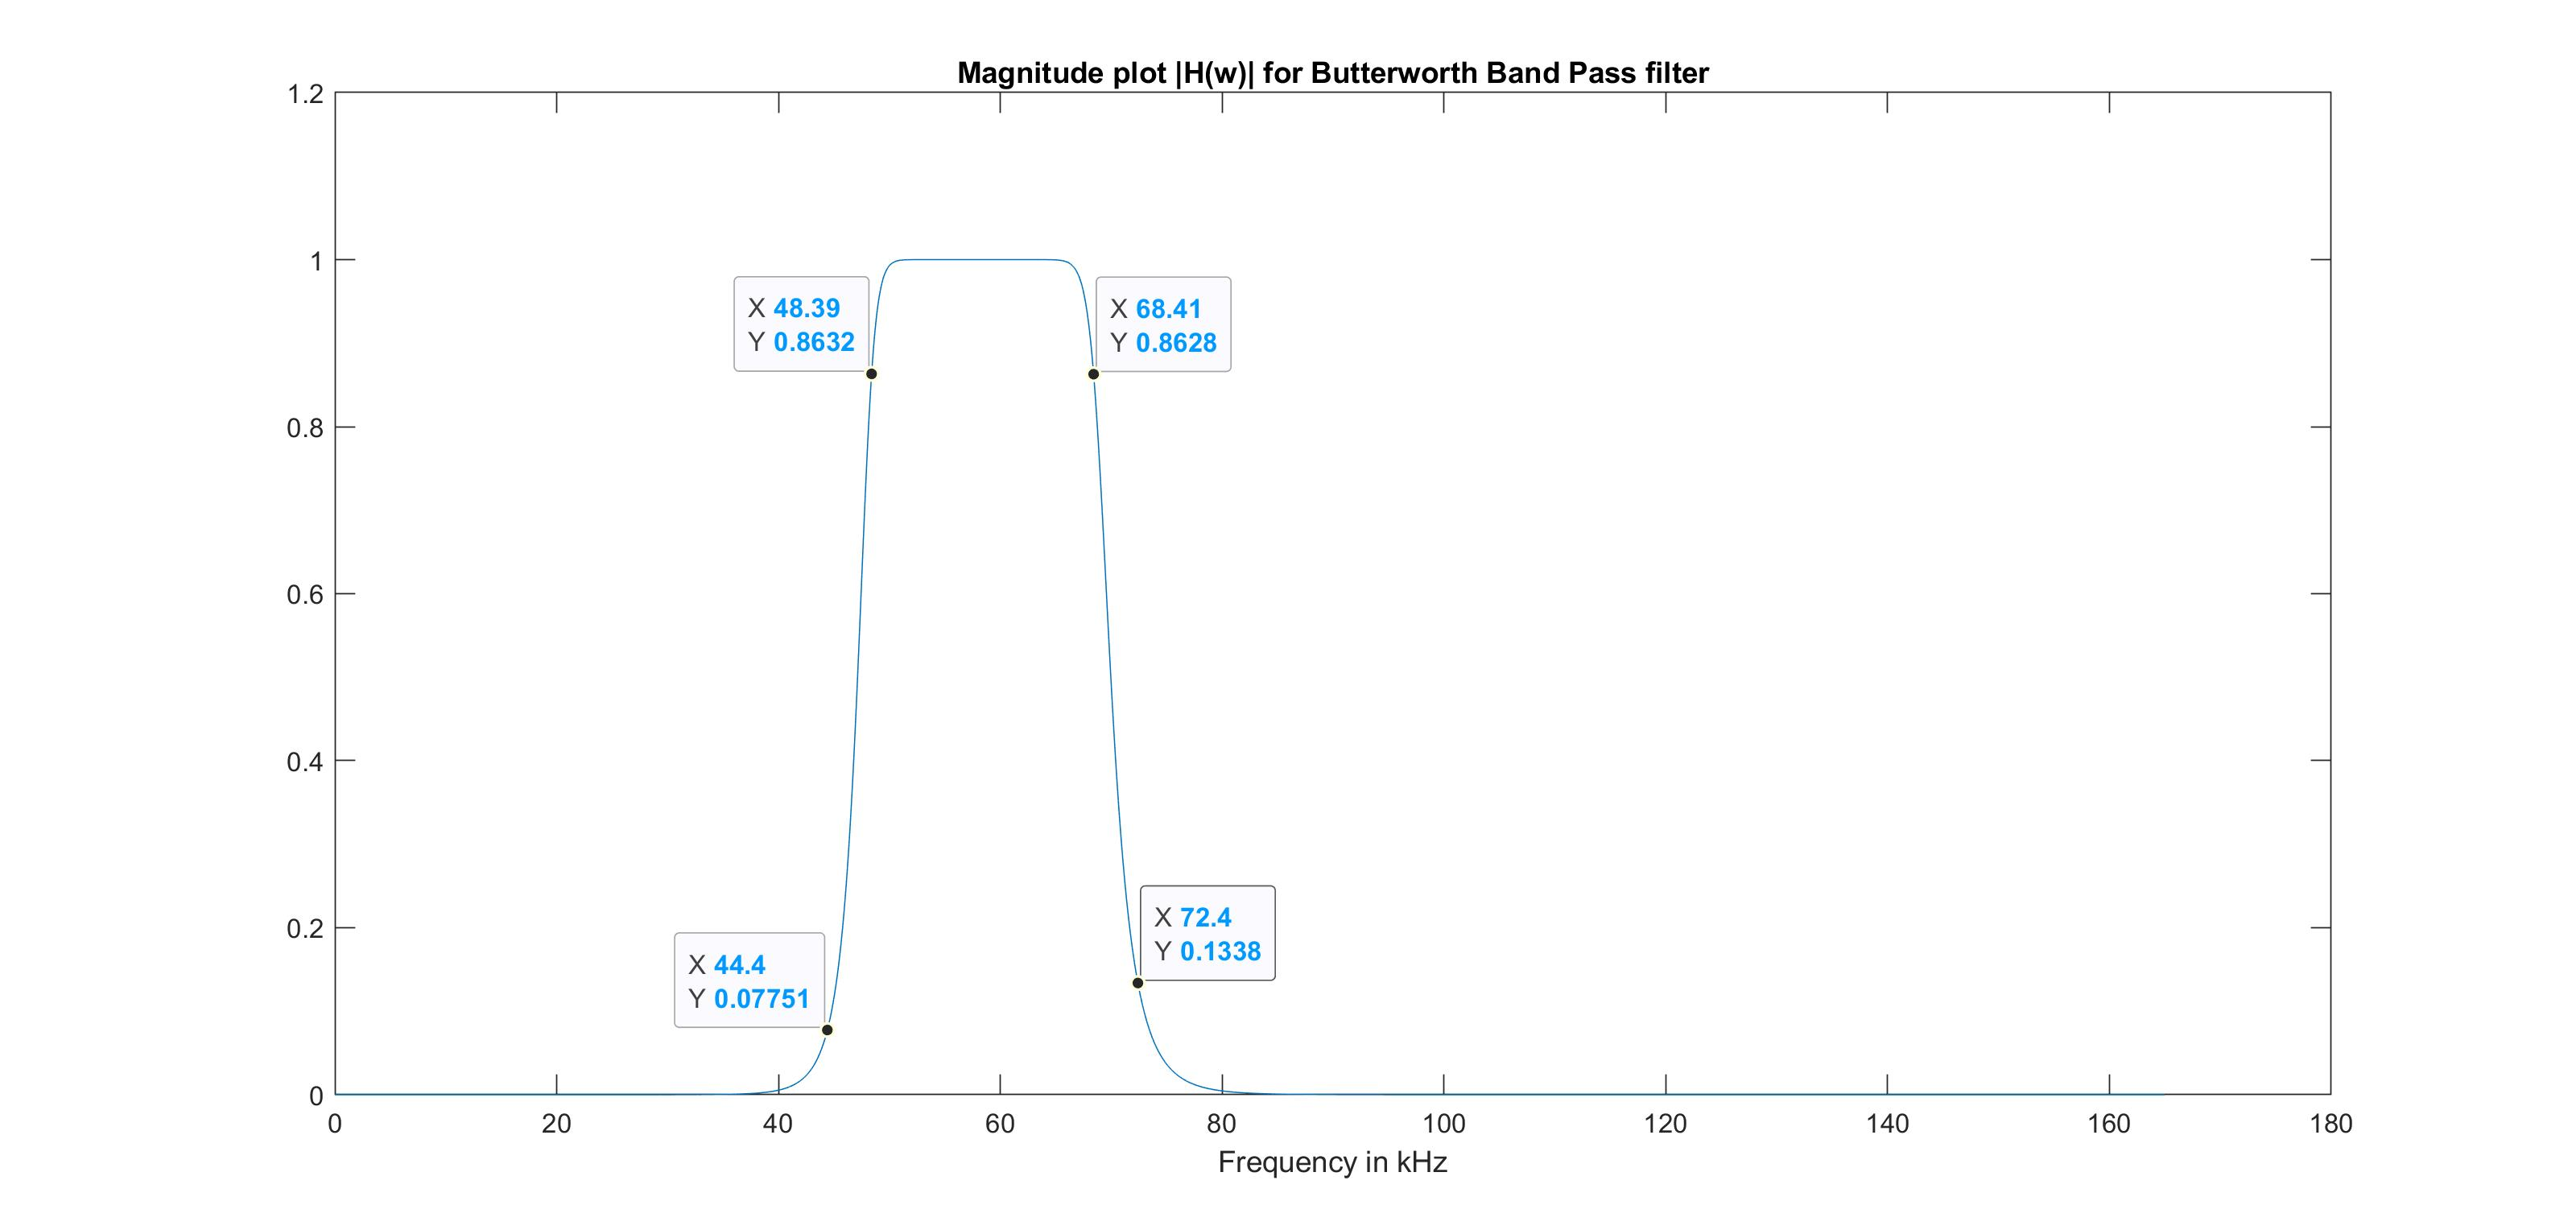
\includegraphics[width = 16cm, height = 10cm]{Filter1DBPF.png}
	\end{figure}

	\color{cyan}
	\subsection{FIR Filter Transfer Function using Kaiser window}
	\color{black}
	Tolerance in both stop band and pass band is given to be 0.15. Therefore, $\delta$ = 0.15, using this we get value of A to be
	\begin{gather*}
		A = -20*log(0.15) = 16.4782 dB
	\end{gather*}
	Since A$<$21, we get the value of the shape parameter of the Kaiser window $\alpha$ = 0. Hence we essentially get a rectangular window, Now the transition bandwidth $\Delta\omega_T$ = $\frac{4}{165} \pi \sim 0.0242\pi$. Using the empirical formula for the length of the window,
	\begin{gather*}
		2Nmin + 1 \ge 1 + \frac{A-8}{2.285\Delta\omega_T}
	\end{gather*}
	This gives us Nmin = 25, which implies the minimum length of the Kaiser window = 51. But this length does not satisfy all the conditions, the least window length satisfying all the conditions found by trial and error on MATLAB is n = 69.\\
	We know the an Ideal Band pass filter can be obtained by subtracting two Ideal Low pass filters, So first we obtain the samples of the Ideal Band Pass filter by subtracting samples of two Low Pass filters of same length as the Kaiser window. Now, we obtain the time domain representation of the final FIR filter by multiplying the Ideal impulse response samples with the Kaiser window.
\begin{figure}[H]
	\centering
	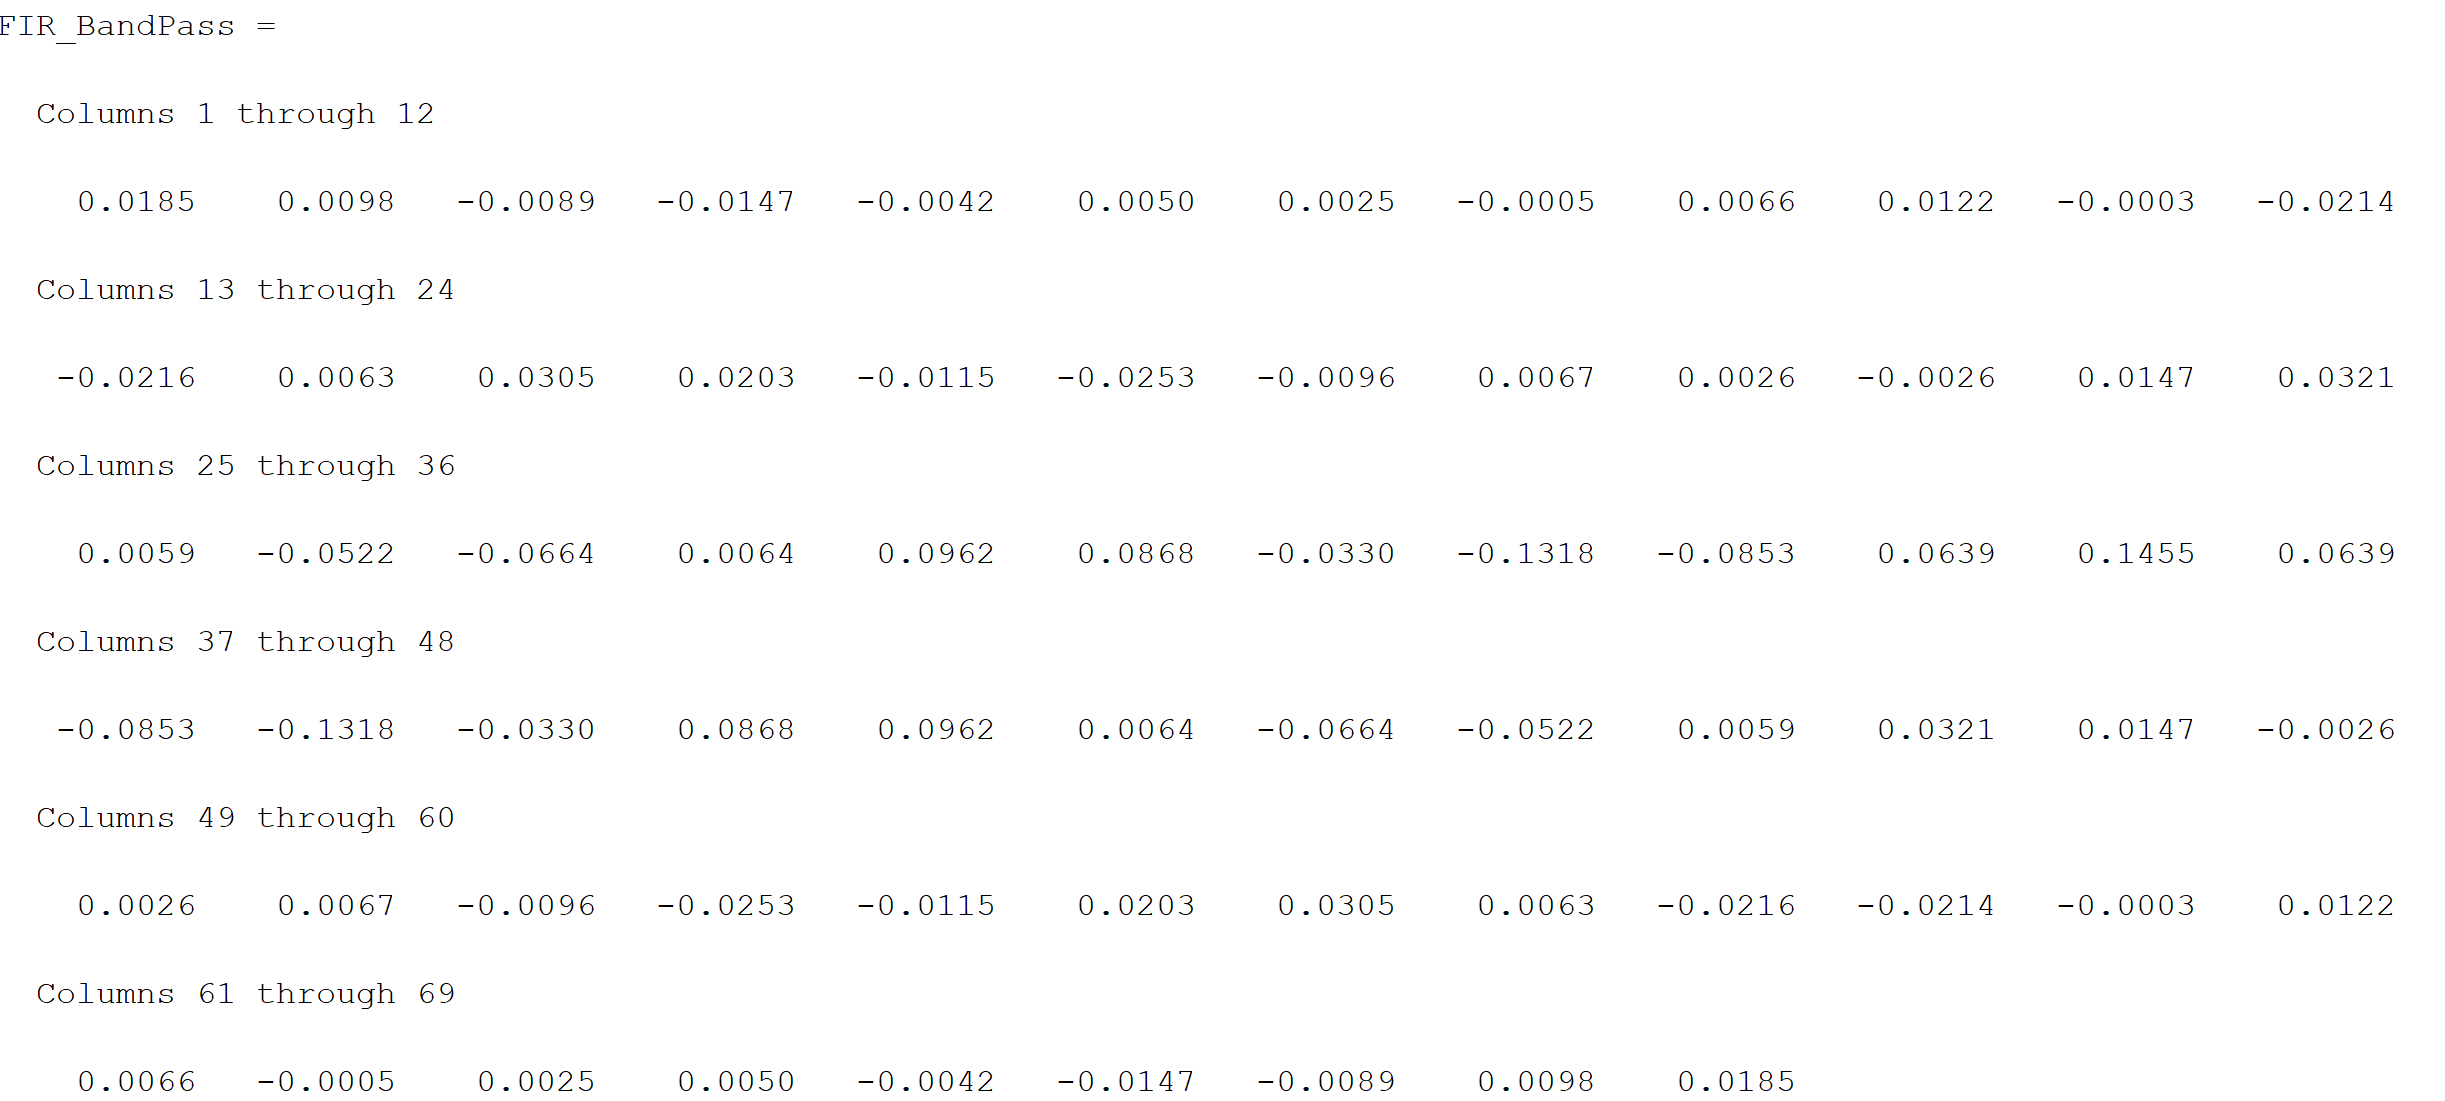
\includegraphics[width  = 18cm]{Filter1hn.png}
	\caption{Time Domain sequence values of the filter}
\end{figure}
\noindent These time domain sequence values are also the coefficients of the Z-transform from 1 to $Z^{-68}$.

\begin{figure}[H]
	\centering
	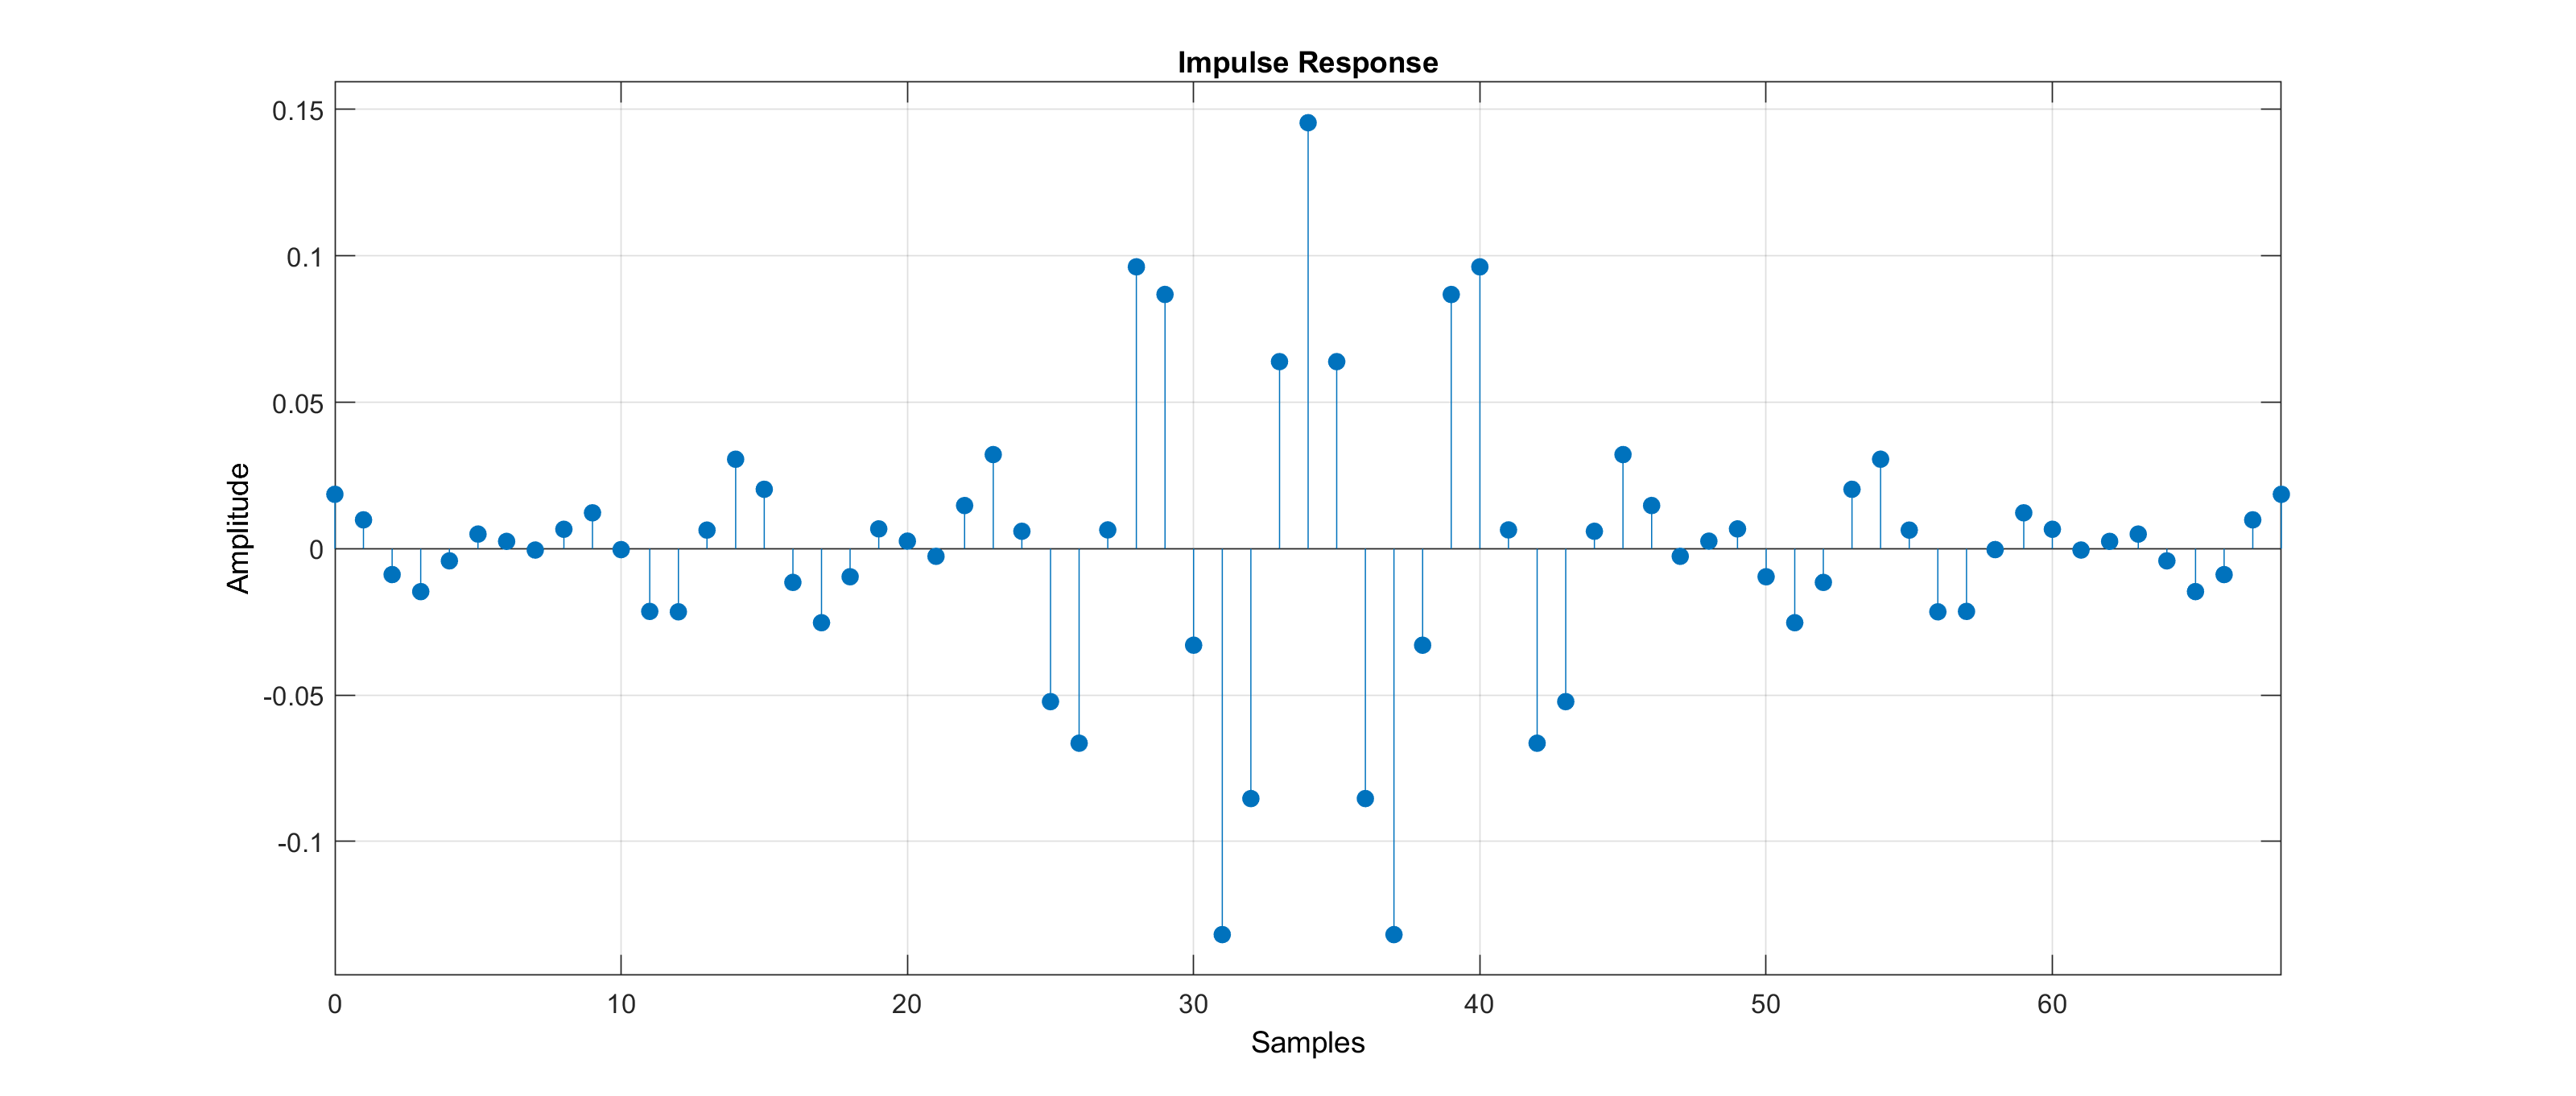
\includegraphics[width = 18cm]{FIRFilter1hn.png}
\end{figure}
\begin{figure}[H]
	\centering
	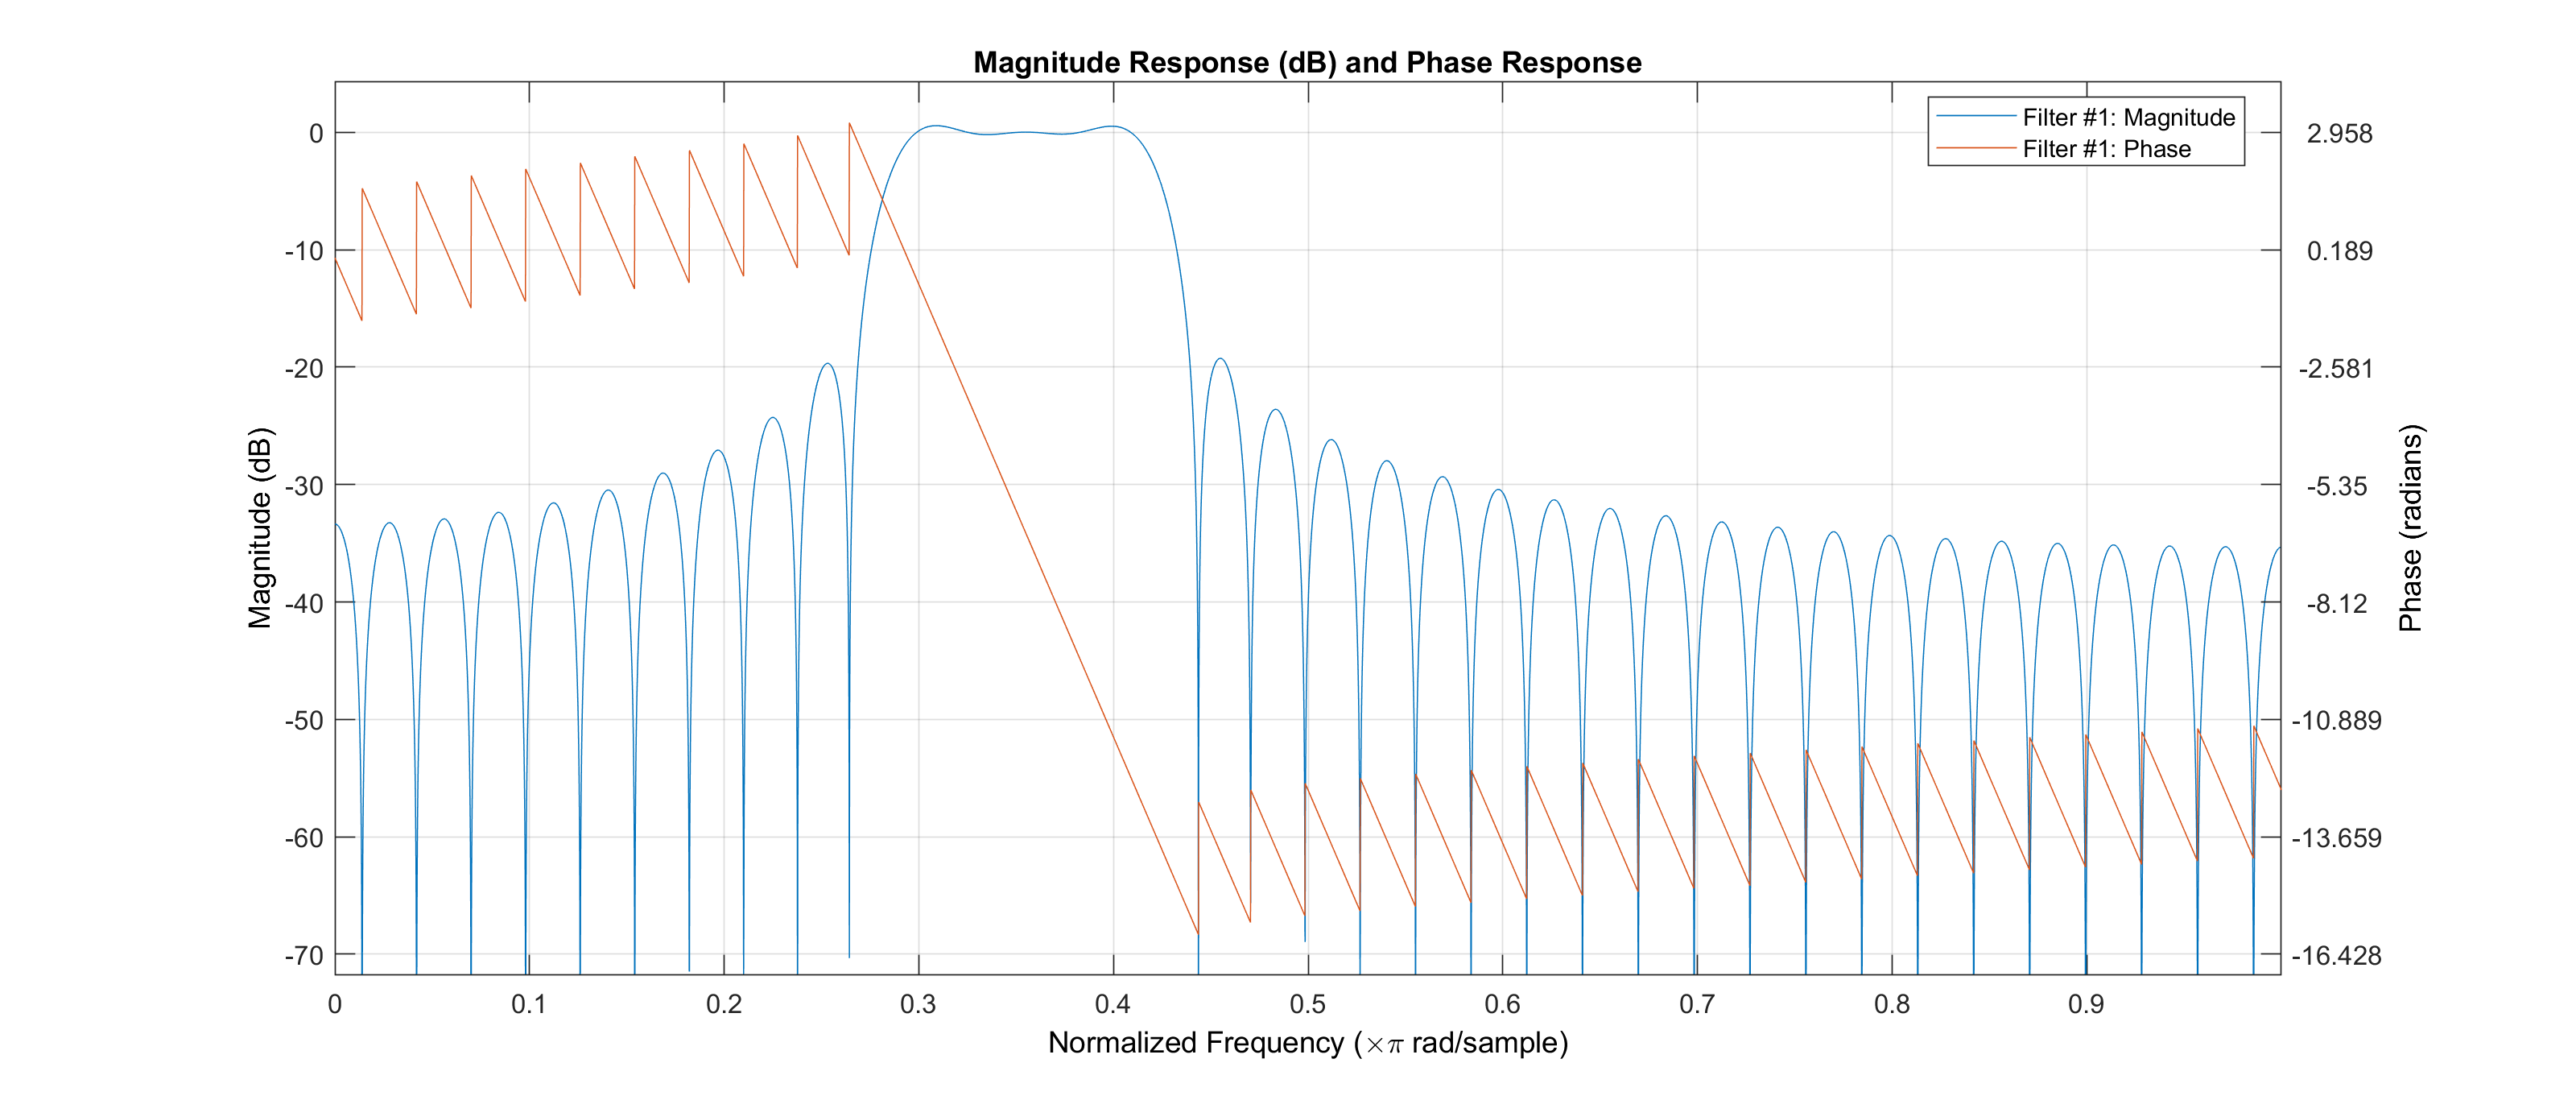
\includegraphics[width = 18cm, height = 10cm]{FIRFilter1MagPhase.png}
\end{figure}
\begin{figure}[H]
	\centering
	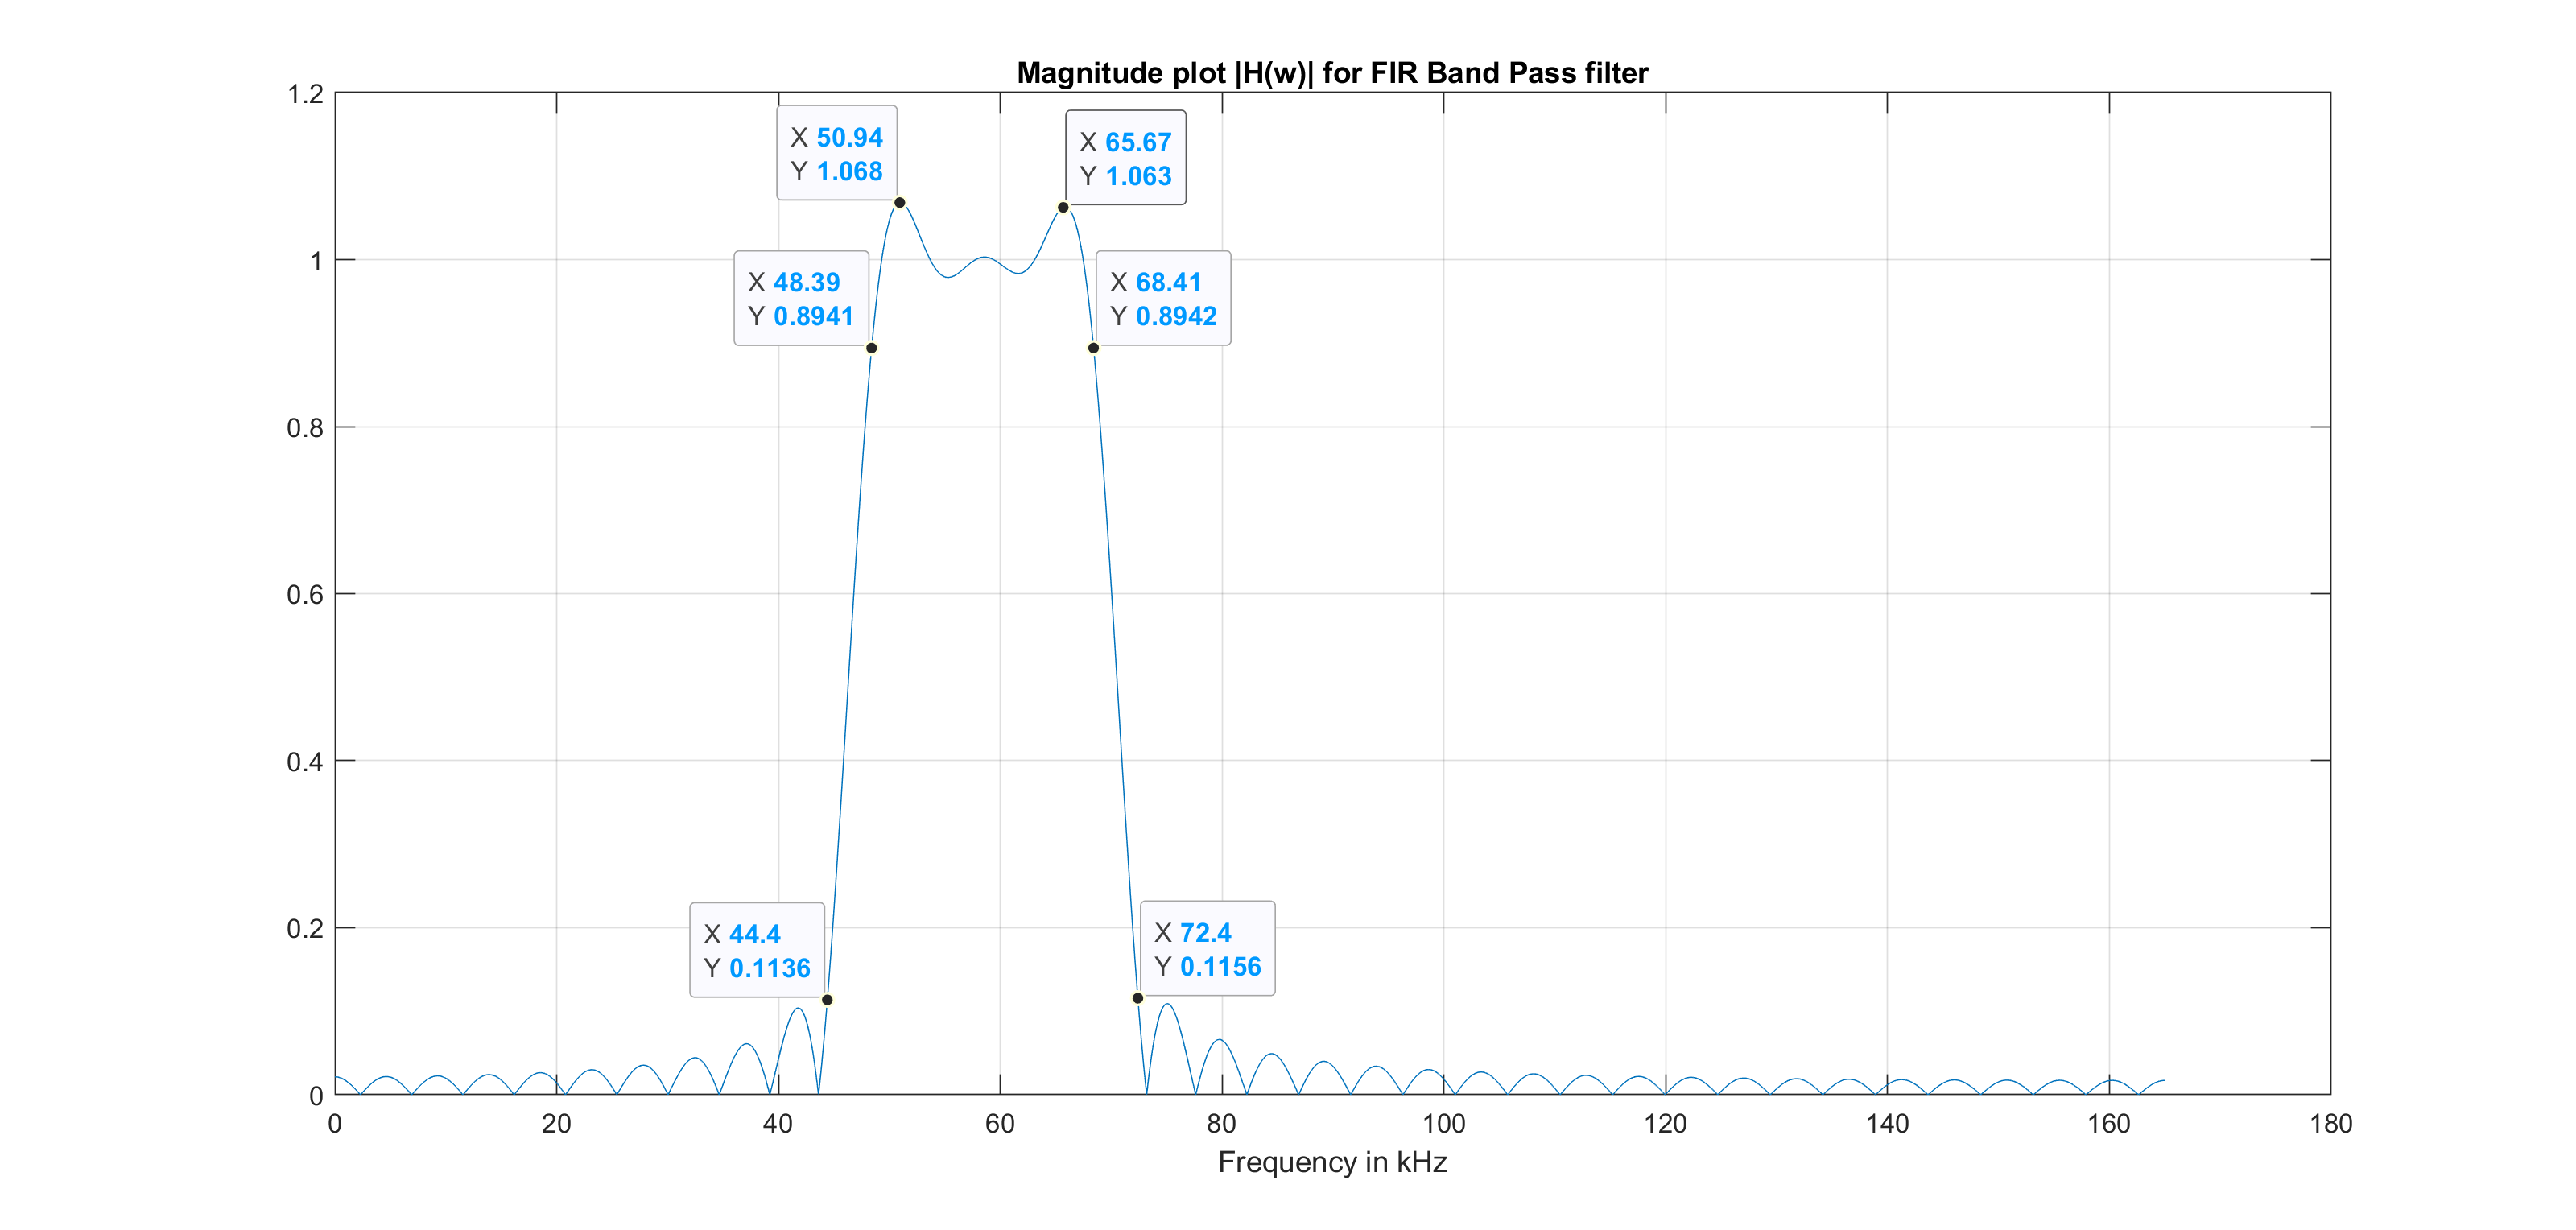
\includegraphics[width = 18cm]{FIRFilter1UBPF.png}
\end{figure}
	
	\color{cyan}
	\subsection{Comparison between FIR and IIR realizations}
	\color{black}
	\begin{itemize}
		\item As discussed in the class, we can see that the FIR filter has linear / Pseudo linear phase in the Pass band where as IIR filter has non-linear phase.
		\item The number of delay lines required for IIR filter is 8+16 = 24, where as for FIR filter we need 68 delay lines.  Hence it is very evident that for the same Filter specifications the FIR filters need a lot more hardware. 
	\end{itemize}
	
	\color{cyan}
	\subsection{Review report}
	\color{black}
	Reviewed Shubham Kar's report
	\begin{itemize}
		\item Specifications were correctly chosen.
		\item All the frequency response specifications are met. We can see this clearly as he marked the critical points on the plots.
		\item All the mandatory parts are done. Although there were some typo's which were corrected.
		
	\end{itemize}
	
	  
	
	
	\newpage
	\color{darkblue}
	\section{Filter 2: Chebyshev Band Stop Filter}
	\color{black}
	\begin{itemize}
		\item Filter Number Assigned = m = 33
		\item Both Pass band and Stop band tolerances are 0.15
		\item Pass Band is Equiripple (as 1 $\le$ m $\le$ 80)
		\item Stop band is Monotonic 
		\item Band-stop Filter
		\item Chebyshev Approximation
		\item The Transition band is 4kHz on either side of the stop band
		\item The input signal is Band limitted to 120kHz and the sampling rate is 260kHz.
	\end{itemize}
	\color{cyan}
	\subsection{Unnormalized Specifications}
	\color{black}
	m = 33\\
	q(m) = 3\\
	r(m) = 33 - 30 = 3\\
	BL(m) = 25 + 1.9 $\times$ 3 + 4.1 $\times$ 3 = 43 kHz\\
	BH(m) = BL(m) + 20 = 63 kHz\\
	
	\noindent Hence the filter specifications for the Band-stop Filter are:
	\begin{itemize}
		\item Stop band is 43 kHz to 63 kHz
		\item Transition band is 4kHz on either side of the Stop band
		\item Pass band is 0 to 39 kHz and 67 kHz to 130 kHz
		\item Tolerances for both bands are 0.15
		\item Pass band: Equiripple
		\item Stop band: Monotonic 
	\end{itemize}
	
	\color{cyan}
	\subsection{Normalized specifications}
	\color{black}
	Given sampling rate  = 260 kHz. Using\\
	\begin{gather*}
		\omega = \frac{2\pi \ast \Omega}{\Omega_s}
	\end{gather*}
	where $\omega$ is the normalized frequency, $\Omega$ is the Un-normalized frequency and $\Omega_s$ is the sampling frequency.
	\begin{itemize}
		\item Stop band is $\frac{43}{130}\pi$ to $\frac{63}{130}\pi$ $\sim$ (0.33$\pi$ to 0.48$\pi$)
		\item Transition band is $\frac{4}{130}\pi$ $\sim$ (0.03$\pi$) on either side of the Stop band
		\item Pass band is 0 to  $\frac{3}{10}\pi$ and $\frac{67}{130}\pi$ to $\pi$  $\sim$ (0 to 0.3$\pi$ and  0.52$\pi$ to $\pi$)
		\item Tolerances for both bands are 0.15
		\item Pass band: Equiripple
		\item Stop band: Monotonic
	\end{itemize}
	
	\color{cyan}
	\subsection{Analog Band-Stop Filter Specifications}
	\color{black}
	Using Bilinear Transformation,
	\begin{gather*}
		\Omega = tan\left(\frac{\omega}{2}\right)
	\end{gather*}
	where $\Omega$ is the analog domain frequency and $\omega$ is the discrete domain frequency\\
	
	\begin{center}
		\begin{tabular}{ |c|c|c|c|c|c|c| }
			\hline
			&&&&&&\\
			Domain & Zero & $\Omega_{P1}$ & $\Omega_{S1}$ &$\Omega_{S2}$& $\Omega_{P2}$& Infinity\\
			&&&&&&\\
			\hline
			&&&&&&\\
			$\omega$ & 0 & $\frac{3}{10}\pi$ & $\frac{43}{130}\pi$& $\frac{63}{130}\pi$& $\frac{67}{130}\pi$& $\pi$\\
			&&&&&&\\
			\hline
			&&&&&&\\
			$\Omega$ & 0 & 0.5095 & 0.572 & 0.9528 & 1.0495 & $\infty$\\
			&&&&&&\\
			\hline
		\end{tabular}
	\end{center}
	
	\noindent Hence the filter specifications for the corresponding analog domain Bandstop Filter are:
	\begin{itemize}
		\item Stop band is 0.572 ($\Omega_{S1}$)  to 0.9528 ($\Omega_{S2}$) 
		\item Pass band is 0 to 0.5095($\Omega_{P1}$) and 1.0495 ($\Omega_{P2}$) to $\infty$
		\item Tolerances for both bands are 0.15
		\item Pass band: Equiripple
		\item Stop band: Monotonic
	\end{itemize}
	
	\color{cyan}
	\subsection{Frequency Transformation in to a Low Pass Filter}
	\color{black}
	Using the Band-Stop Transformation
	\begin{gather*}
		\Omega_L = \frac{B\Omega}{\Omega_0^2 - \Omega^2}\\\\
		\Omega_0 = \sqrt{\Omega_{P1} \Omega_{P2}} = 0.7313\\\\
		B = \Omega_{P2} - \Omega_{P1} = 0.54
	\end{gather*}
	
	\begin{center}
		\begin{tabular}{ |c|c|c|c|c|c|c|c|c| }
			\hline
			&&&&&&&&\\
			Domain & Zero & $\Omega_{P1}$ & $\Omega_{S1}$ &$\Omega_0^-$ &$\Omega_0^+$ & $\Omega_{S2}$& $\Omega_{P2}$ & Infinity\\
			&&&&&&&&\\
			\hline
			&&&&&&&&\\
			$\Omega$ & 0$^+$ & 0.5095 & 0.572 &0.7313 &0.7313&0.9528& 1.0495 & +$\infty$\\
			&&&&&&&&\\
			\hline
			&&&&&&&&\\
			$\Omega_L$ & 0$^+$ & 1 & 1.4879 & +$\infty$ & -$\infty$ & -1.3792 & -1 & 0$^-$\\
			&&&&&&&&\\
			\hline
			&&&&&&&&\\
			Domain& Zero & $\Omega_{LP1}$ & $\Omega_{LS1}$ &+Infinity &-Infinity & $\Omega_{LS2}$& $\Omega_{LP2}$ &Zero\\
			&&&&&&&&\\
			\hline
		\end{tabular}
	\end{center}
	
	\color{cyan}
	\subsection{Analog Low Pass Filter Specification}
	\color{black}
	Hence the Frequency Transformed Low-Pass Filter Specifications are:
	\begin{itemize}
		\item Pass band edge is at 1 ($\Omega_{LP}$)
		\item Stop band edge = min (-$\Omega_{LS2}$, $\Omega_{LS1}$) = 1.3792 ($\Omega_{LS}$)
		\item Tolerances = 0.15 for both Stop band and Pass band
		\item Pass band: Equiripple
		\item Stop band: Monotonic
	\end{itemize}
	
	
	\color{cyan}
	\subsection{Analog Low Pass Transfer function}
	\color{black}
	Using, Chebyshev Approximation, As Tolerances of both Pass Band and Stop Band are 0.15.
	\begin{gather*}
		D_1 = \frac{1}{(1-\delta_1)^2} - 1 = 0.3841\\
		D_2 = \frac{1}{\delta_2^2} - 1 = 43.4444
	\end{gather*}
	\begin{gather*}
		H_{analog,LPF}^2(j\Omega) = \frac{1}{1+\epsilon^2C_{N}^2(\frac{\Omega}{\Omega_{LP}})} 
	\end{gather*}
	Choosing the parameter $\epsilon$ of Chebyshev filter to be $\sqrt{D_1}$, the inequality for Order N is 
	\begin{gather*}
		N_{min} = \ceil[\Bigg]{ \frac{cosh^{-1}\left(\sqrt{\frac{D2}{D1}}\right)}{cosh^{-1}\left(\frac{\Omega_{LS}}{\Omega_{LP}}\right)}} \\
		N_{min} = 4
	\end{gather*}
	Hence, the poles of the transfer function can be obtained by,
	\begin{gather*}
		1 + D_1cosh^2\left(N_{min}cosh^{-1}\left(\frac{s}{j\Omega_{LP}}\right)\right) = 1 + 0.3841cosh^2\left(4cosh^{-1}\left(\frac{s}{j}\right)\right) = 0
	\end{gather*}
	Using Wolfram to plot the poles,
	\begin{figure}[H]
		\centering
		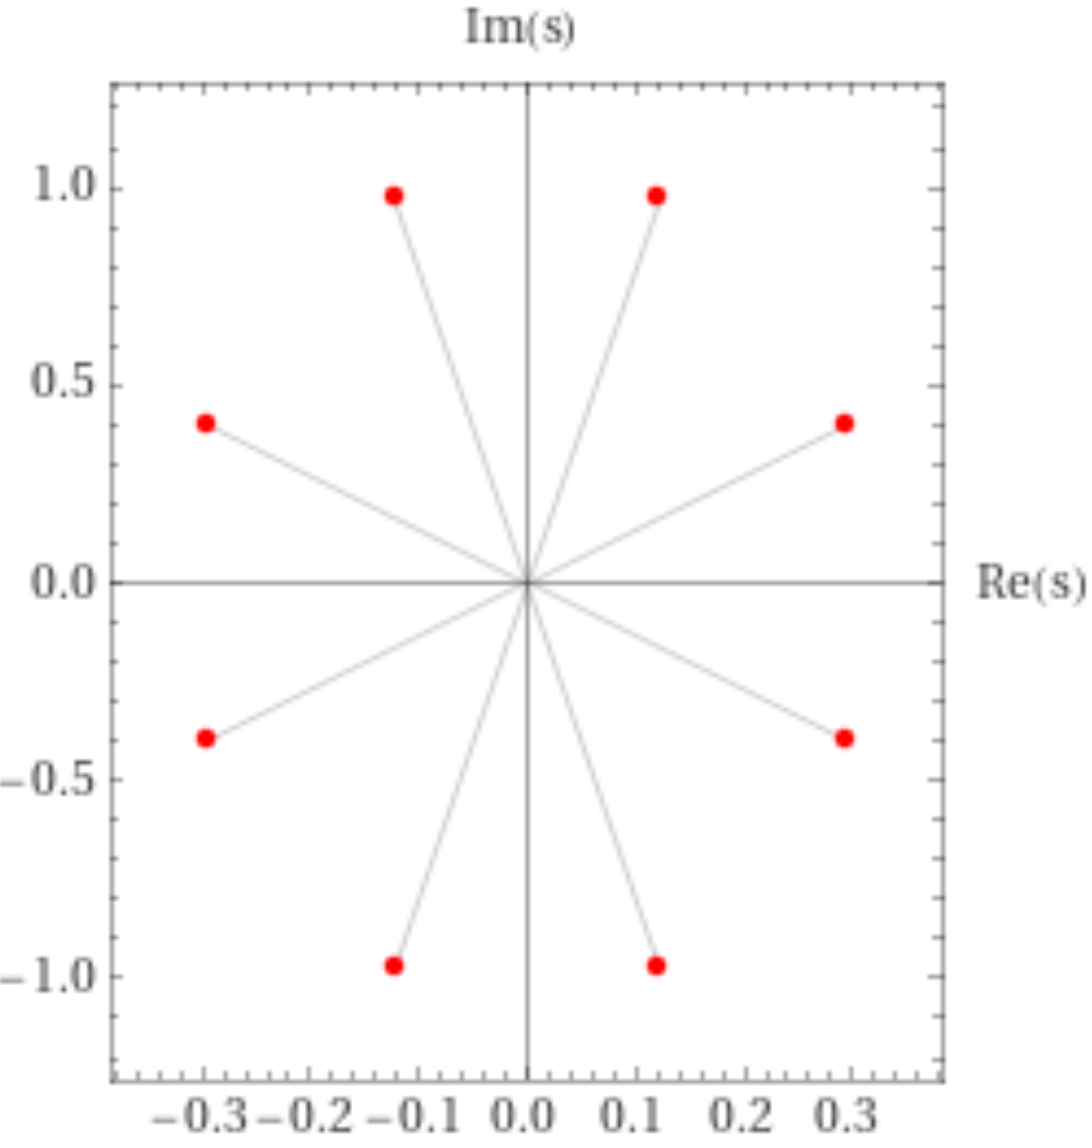
\includegraphics[width = 6cm, height= 5cm]{Chebyshevpoles.png}
	\end{figure}
	\noindent Note that to keep the stability and causality, we need to choose only the poles that lie on the left half plane i.e, Re(s) $<$ 0.

	\begin{verbatim*}
		p1=-0.12216+0.96981i
		p2=-0.29492+0.40171i
		p3=-0.29492-0.40171i
		p4=-0.12216-0.96981i
	\end{verbatim*}
	Using these four poles and the fact that N is even the transfer function Low pass analog filter,
	\begin{gather*}
		H_{analog,LPF}(s_{L}) = \frac{(-1)^4p_1p_2p_3p_4}{\sqrt{1 + D_1}(s_L - p_1)(s_L - p_2)(s_L - p_3)(s_L - p_4)}
	\end{gather*}
	
	\noindent Note that since it is even order, we take the DC order to be $\frac{1}{\sqrt{1+\epsilon^2}}$
	\begin{gather*}
		H_{analog,LPF}(s_{L}) = \frac{0.2011}{s_L^4 + 0.8342s_L^3 + 1.3451s_L^2 + 0.6226s_L + 0.2366}	
	\end{gather*}
	
	\begin{figure}[H]
		\centering
		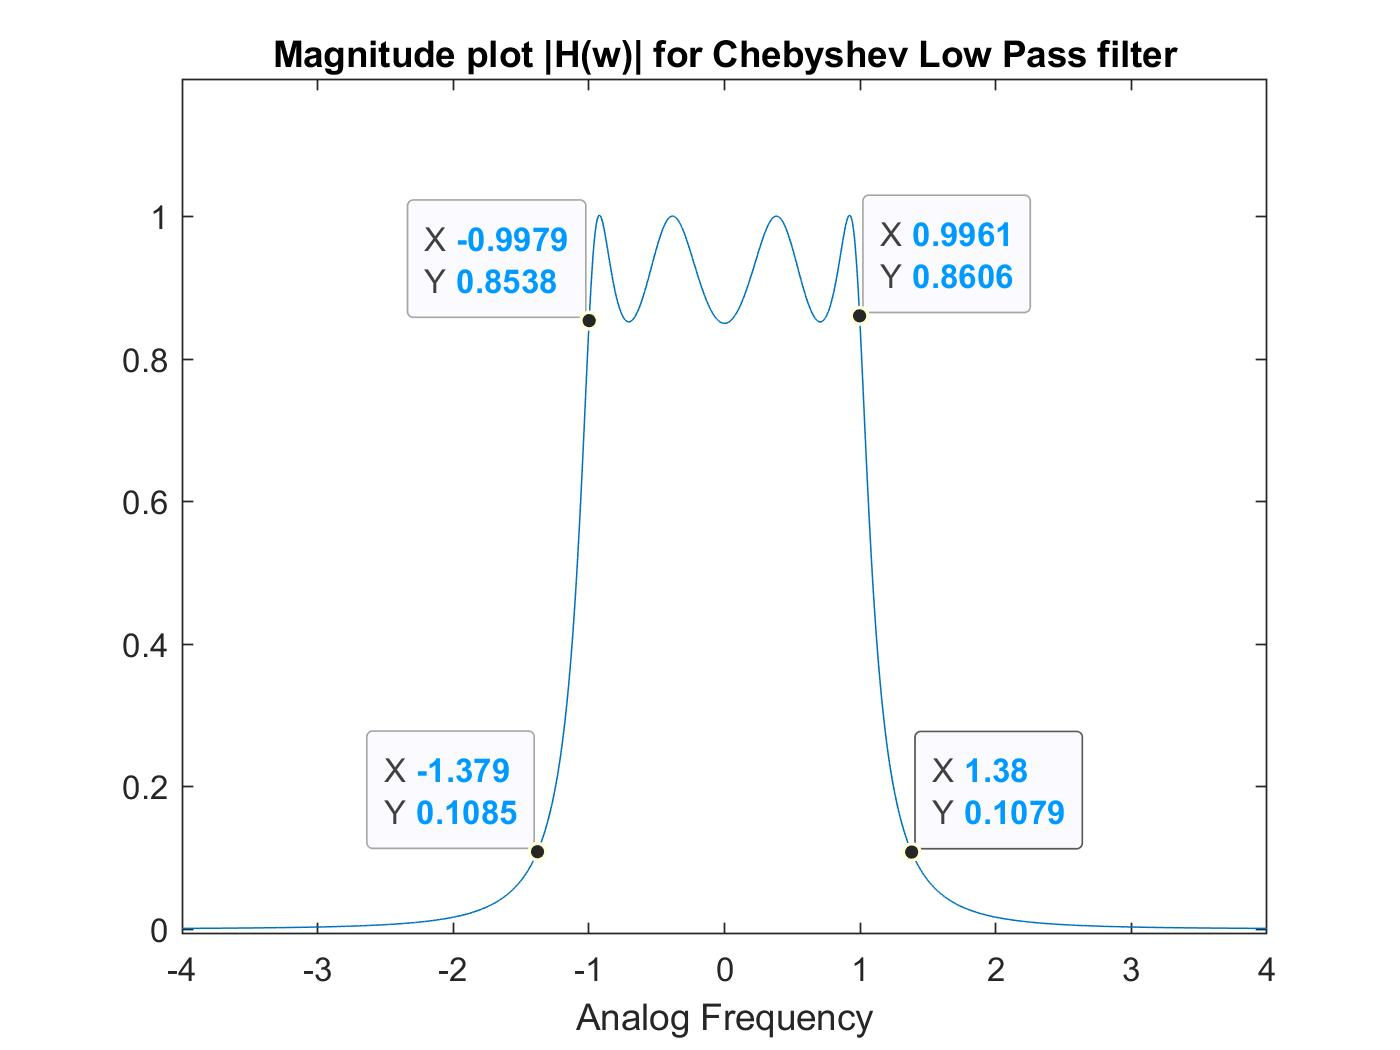
\includegraphics[width = 12cm]{Filter2ALPF.jpg}
	\end{figure}

	\color{cyan}
	\subsection{Analog Band Stop Transfer function}
	\color{black}
	
	Using the Band stop transformation:
	\begin{gather*}
		s_L = \frac{Bs}{s^2 + \Omega_0^2}
	\end{gather*}
	Substituting the values B = 0.54 and $\Omega_0$ = 0.7313,
	\begin{gather*}
		s_L = \frac{0.54s}{s^2 + 0.535}
	\end{gather*}
	Substituting this back into $H_{analog,LPF}$, we get $H_{analog,BSF}$ as
	\begin{gather*}
		\frac{0.85s^8 + 1.8182s^6 + 1.4585s^4 + 0.52s^2 + 0.0695}{s^8 + 1.4211s^7 + 3.797s^6 + 2.835s^5 + 3.8485s^4 + 1.5161s^3 + 1.0859s^2 + 0.2173s + 0.0818}	
	\end{gather*}
	\begin{figure}[H]
		\centering
		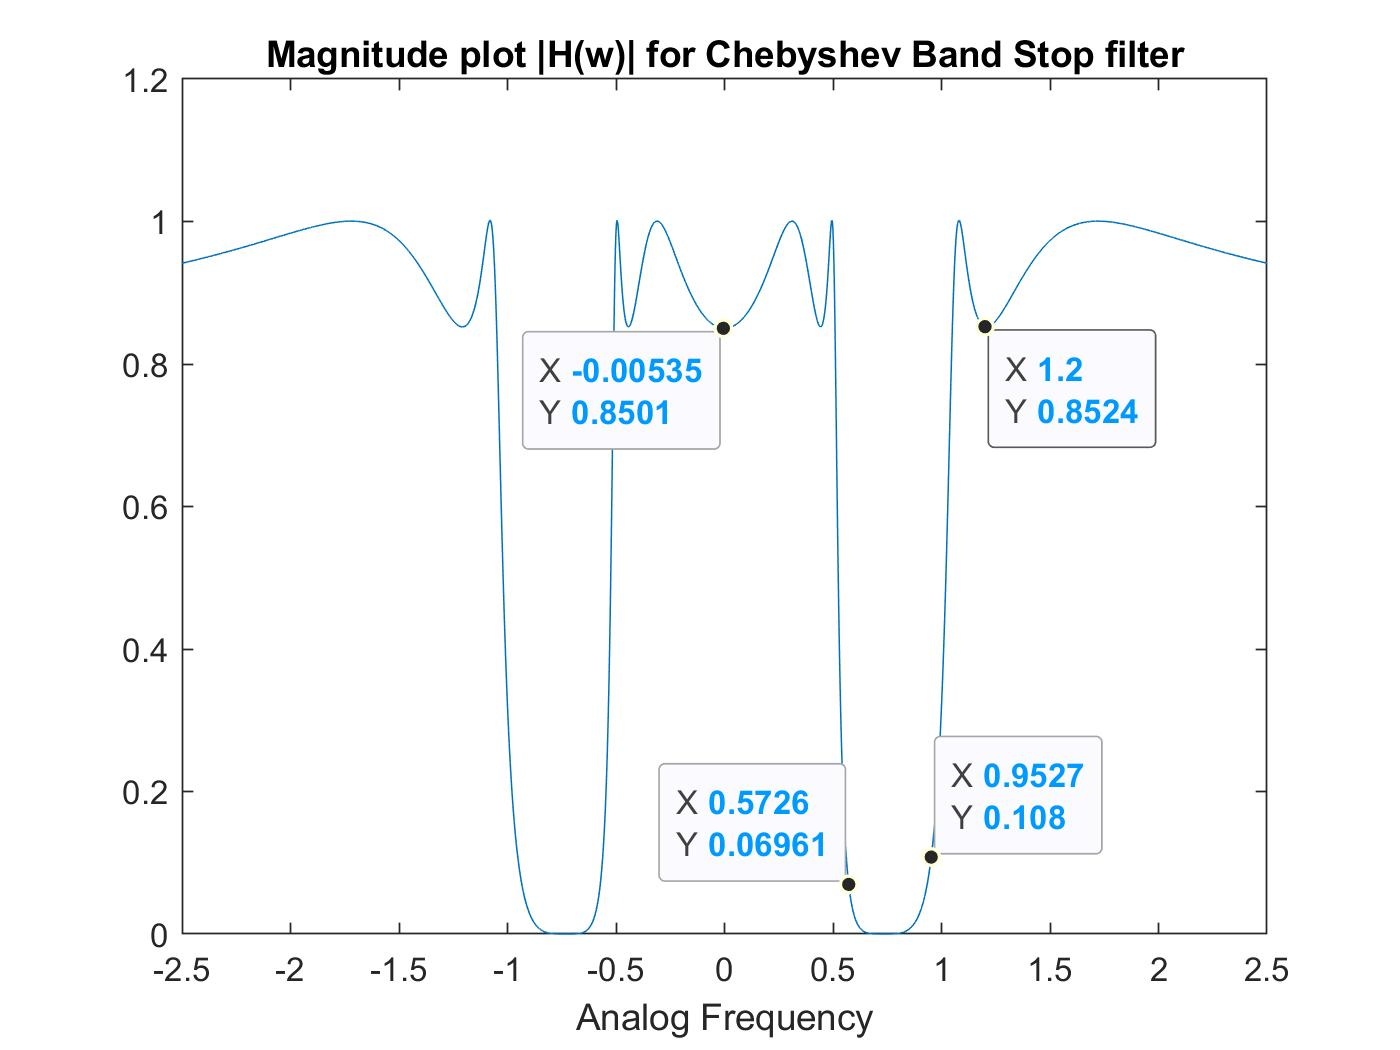
\includegraphics[width = 12cm, trim=1cm 0cm 1cm 0cm, clip]{Filter2ABSF.jpg}
	\end{figure}

	\color{cyan}
	\subsection{Discrete time Band Stop Transfer function}
	\color{black}
	Using the Bilinear Transformation:
	\begin{gather*}
		s = \frac{1-z^{-1}}{1+z^{-1}}
	\end{gather*}
	Substituting this back into $H_{Analog,BSF}(s)$, we get $H_{digital,BSF}$ as
	\begin{gather*}
		\frac{0.298 - 0.724z^{-1} + 1.852z^{-2} - 2.437z^{-3} + 3.147z^{-4} - 2.437z^{-5} + 1.852z^{-6} - 0.724z^{-7}	+ 0.298z^{-8}}{1 - 1.775z^{-1} + 3.0794z^{-2} - 3.133z^{-3} + 3.163z^{-4} - 2.002z^{-5} + 1.278z^{-6} - 0.527z^{-7} + 0.242z^{-8}}
	\end{gather*}
	\begin{figure}[H]
		\centering
		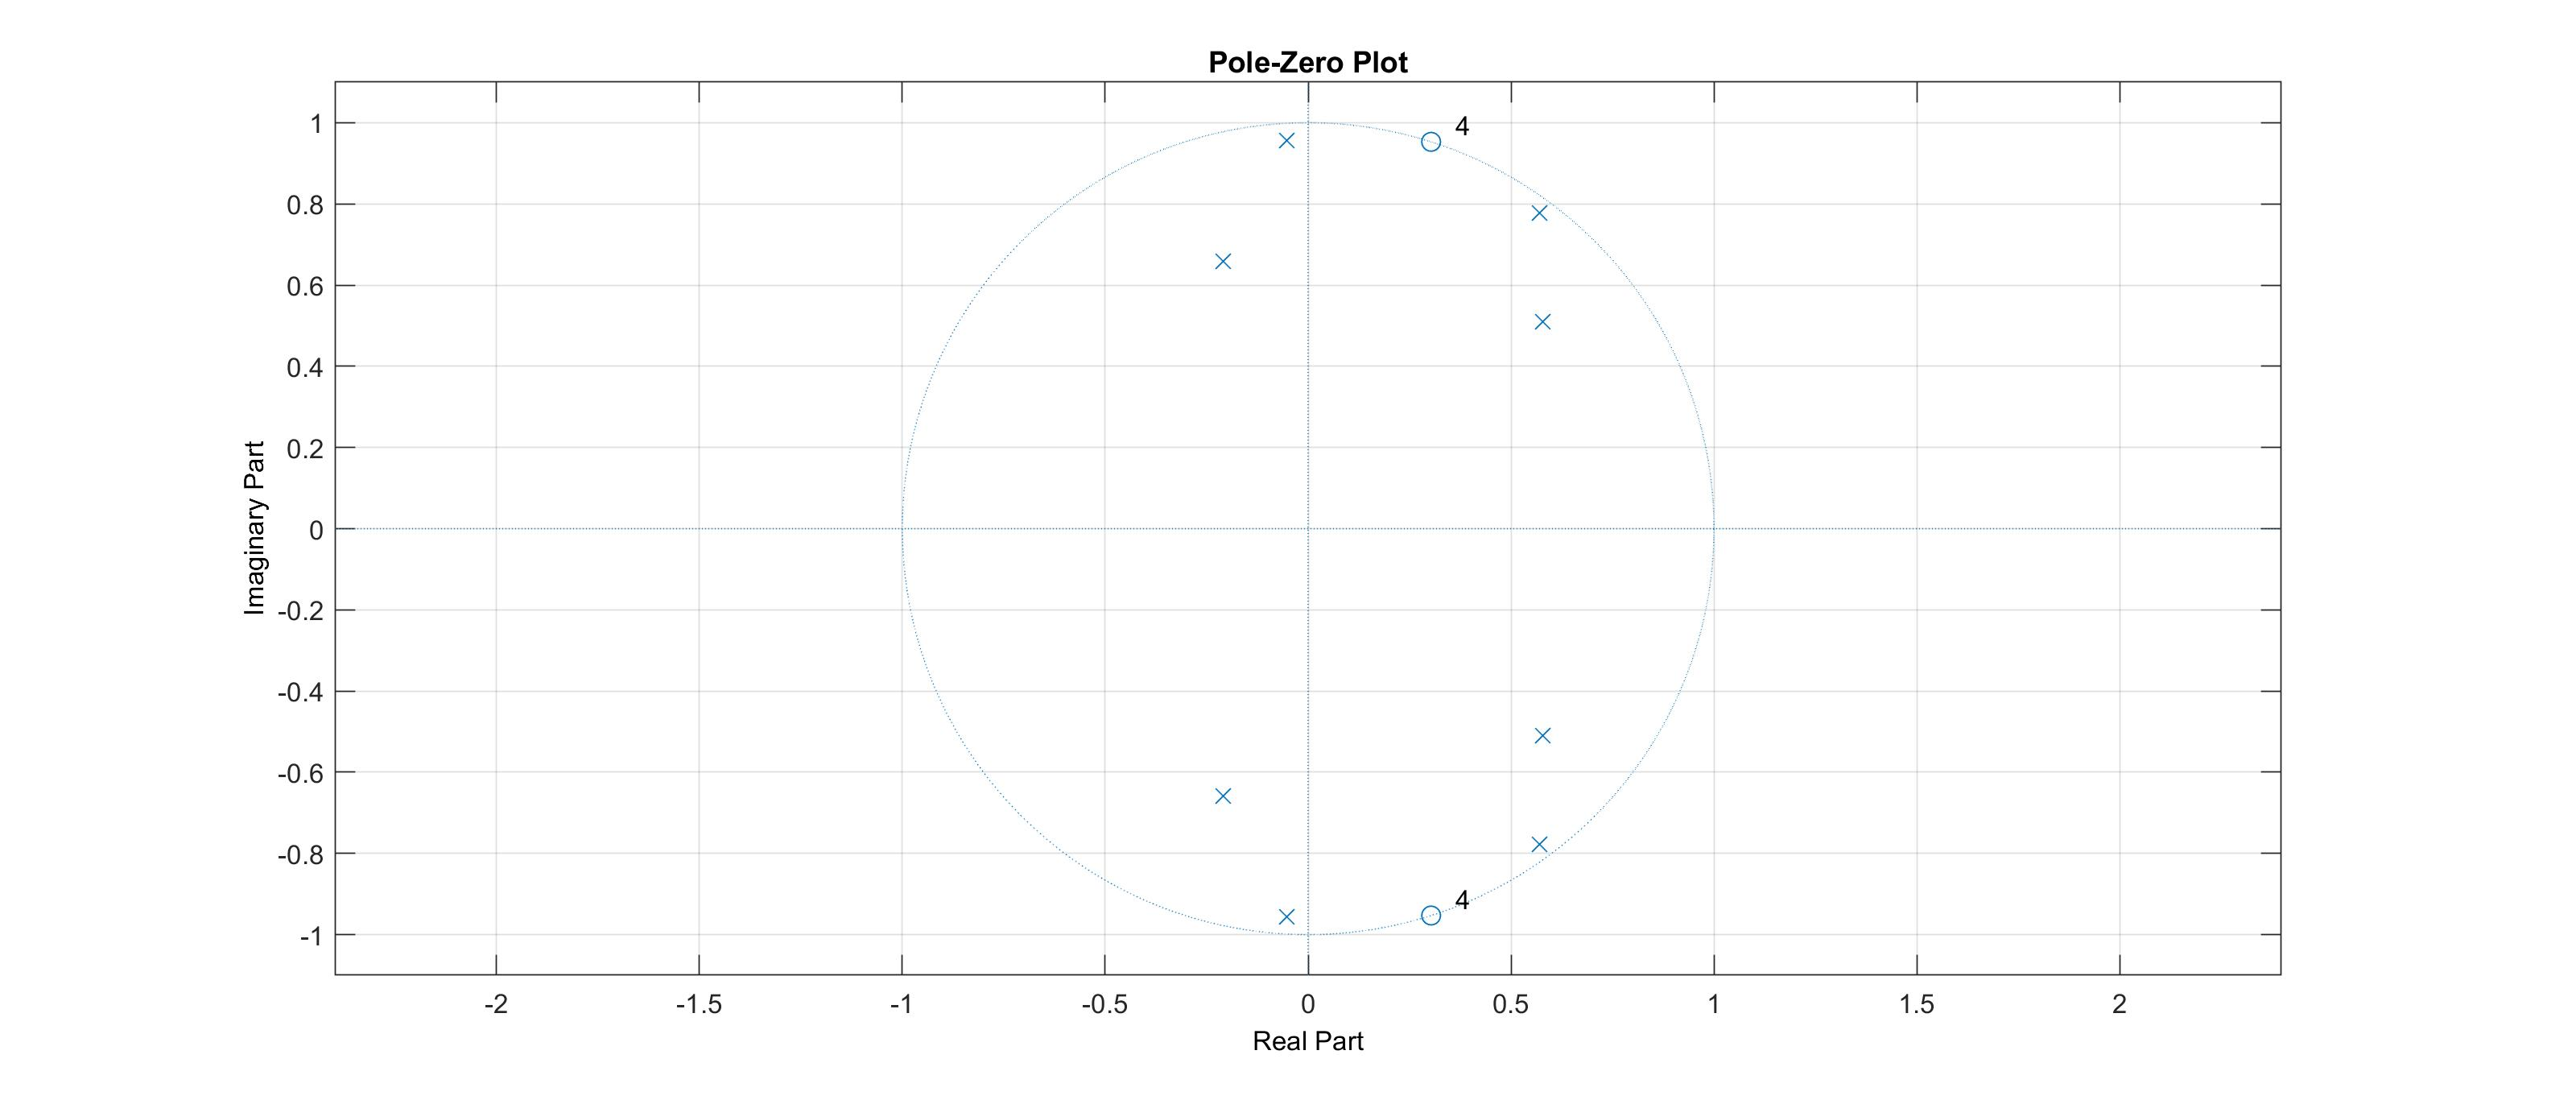
\includegraphics[width = 18cm]{Filter2PZ.jpg}
	\end{figure}
	
	\begin{figure}[H]
		\centering
		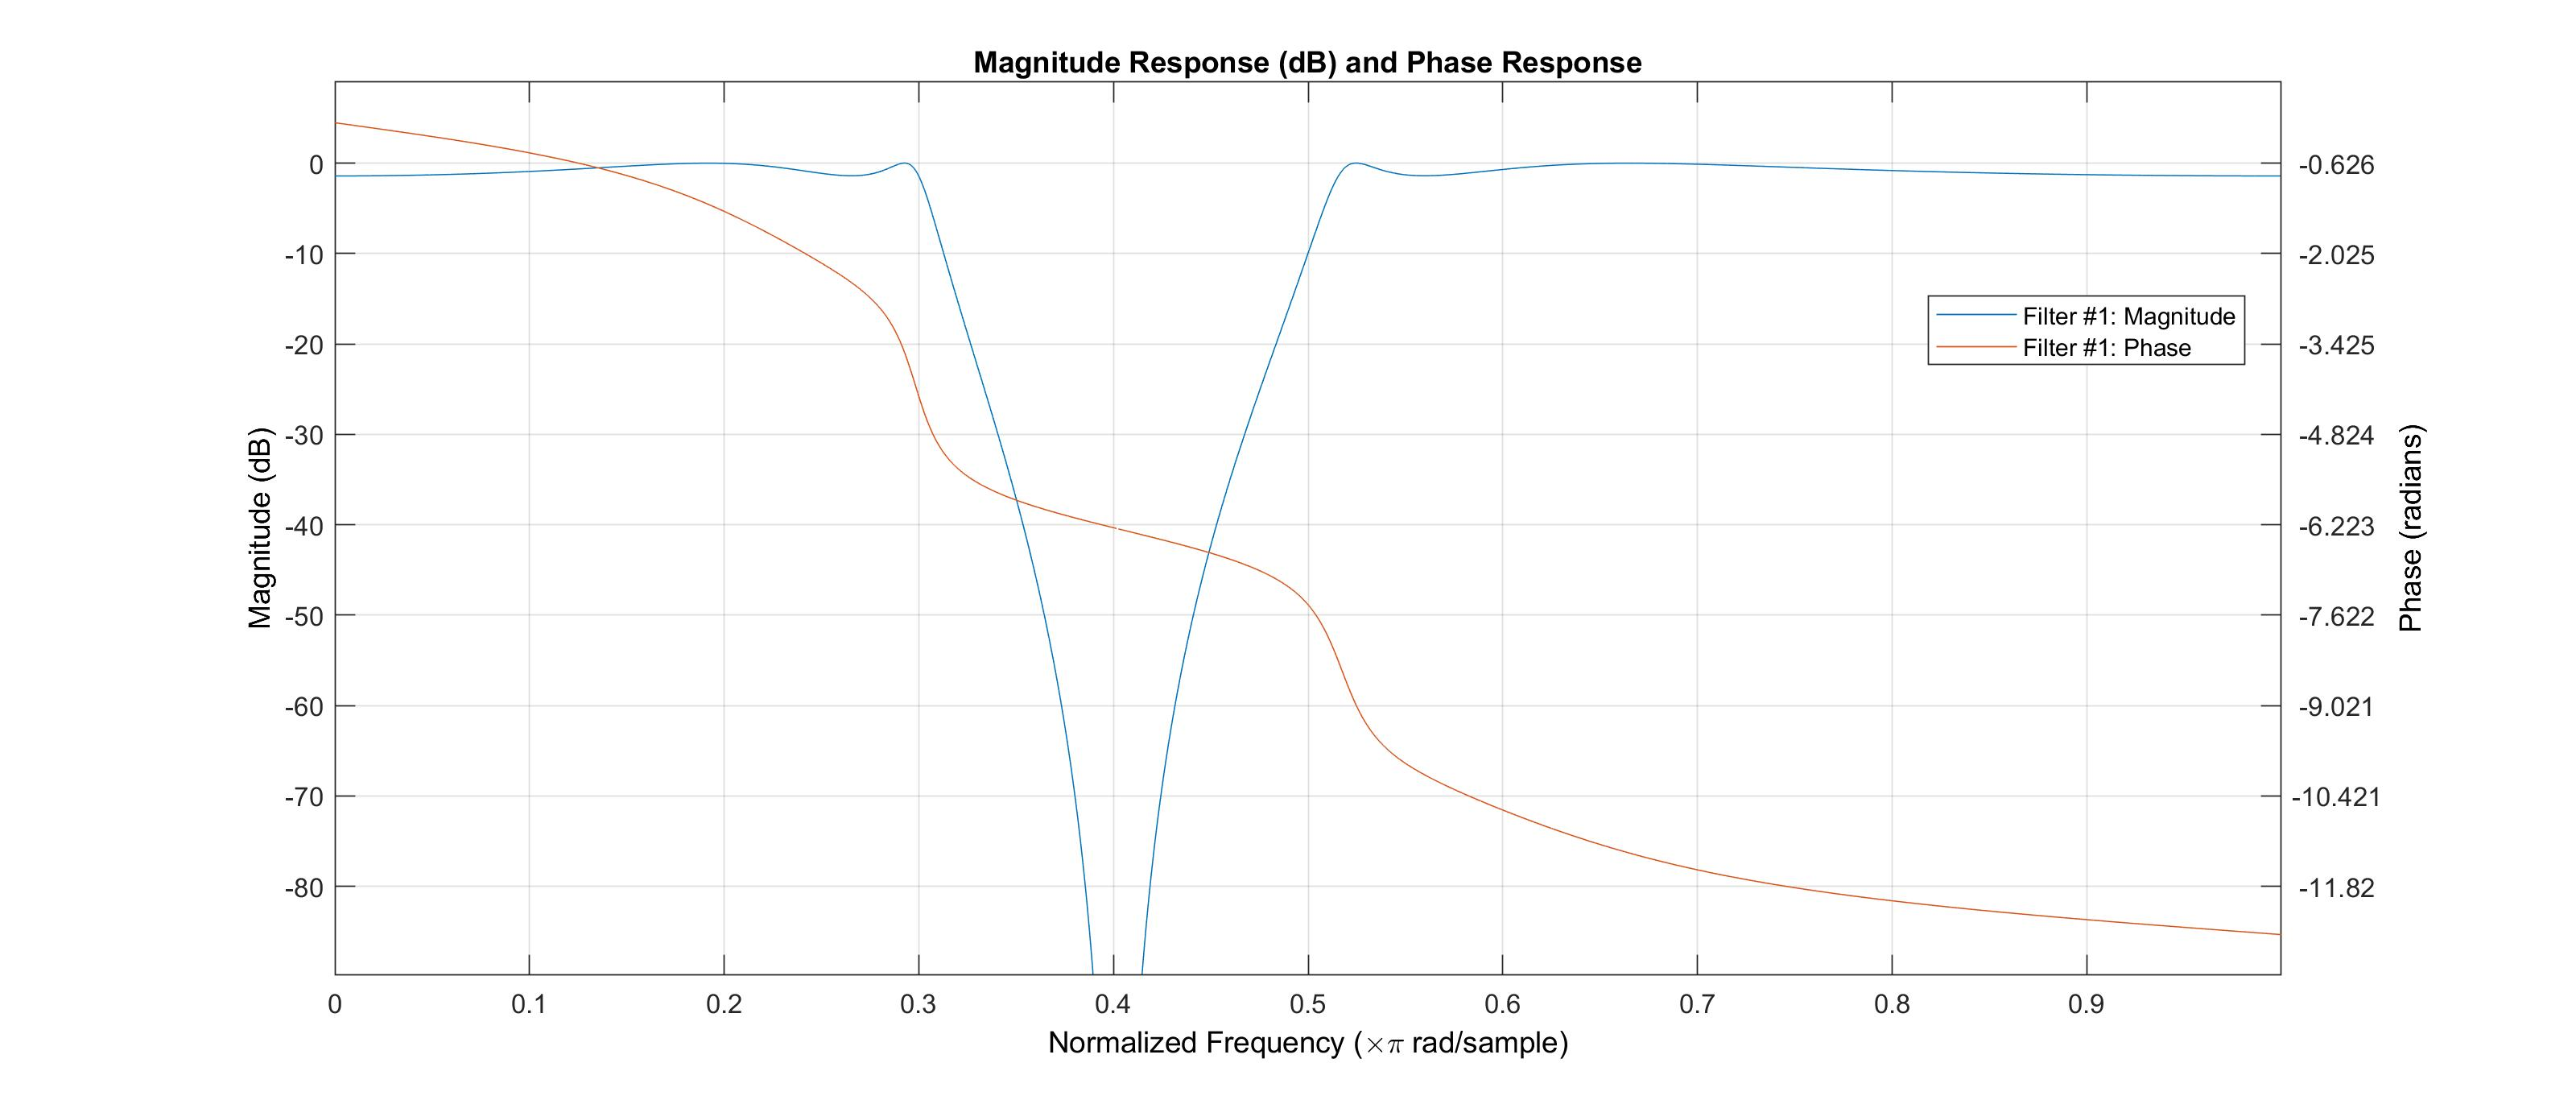
\includegraphics[width = 18cm, height = 10cm]{Filter2MagPhase.jpg}
	\end{figure}
	\begin{figure}[H]
		\centering
		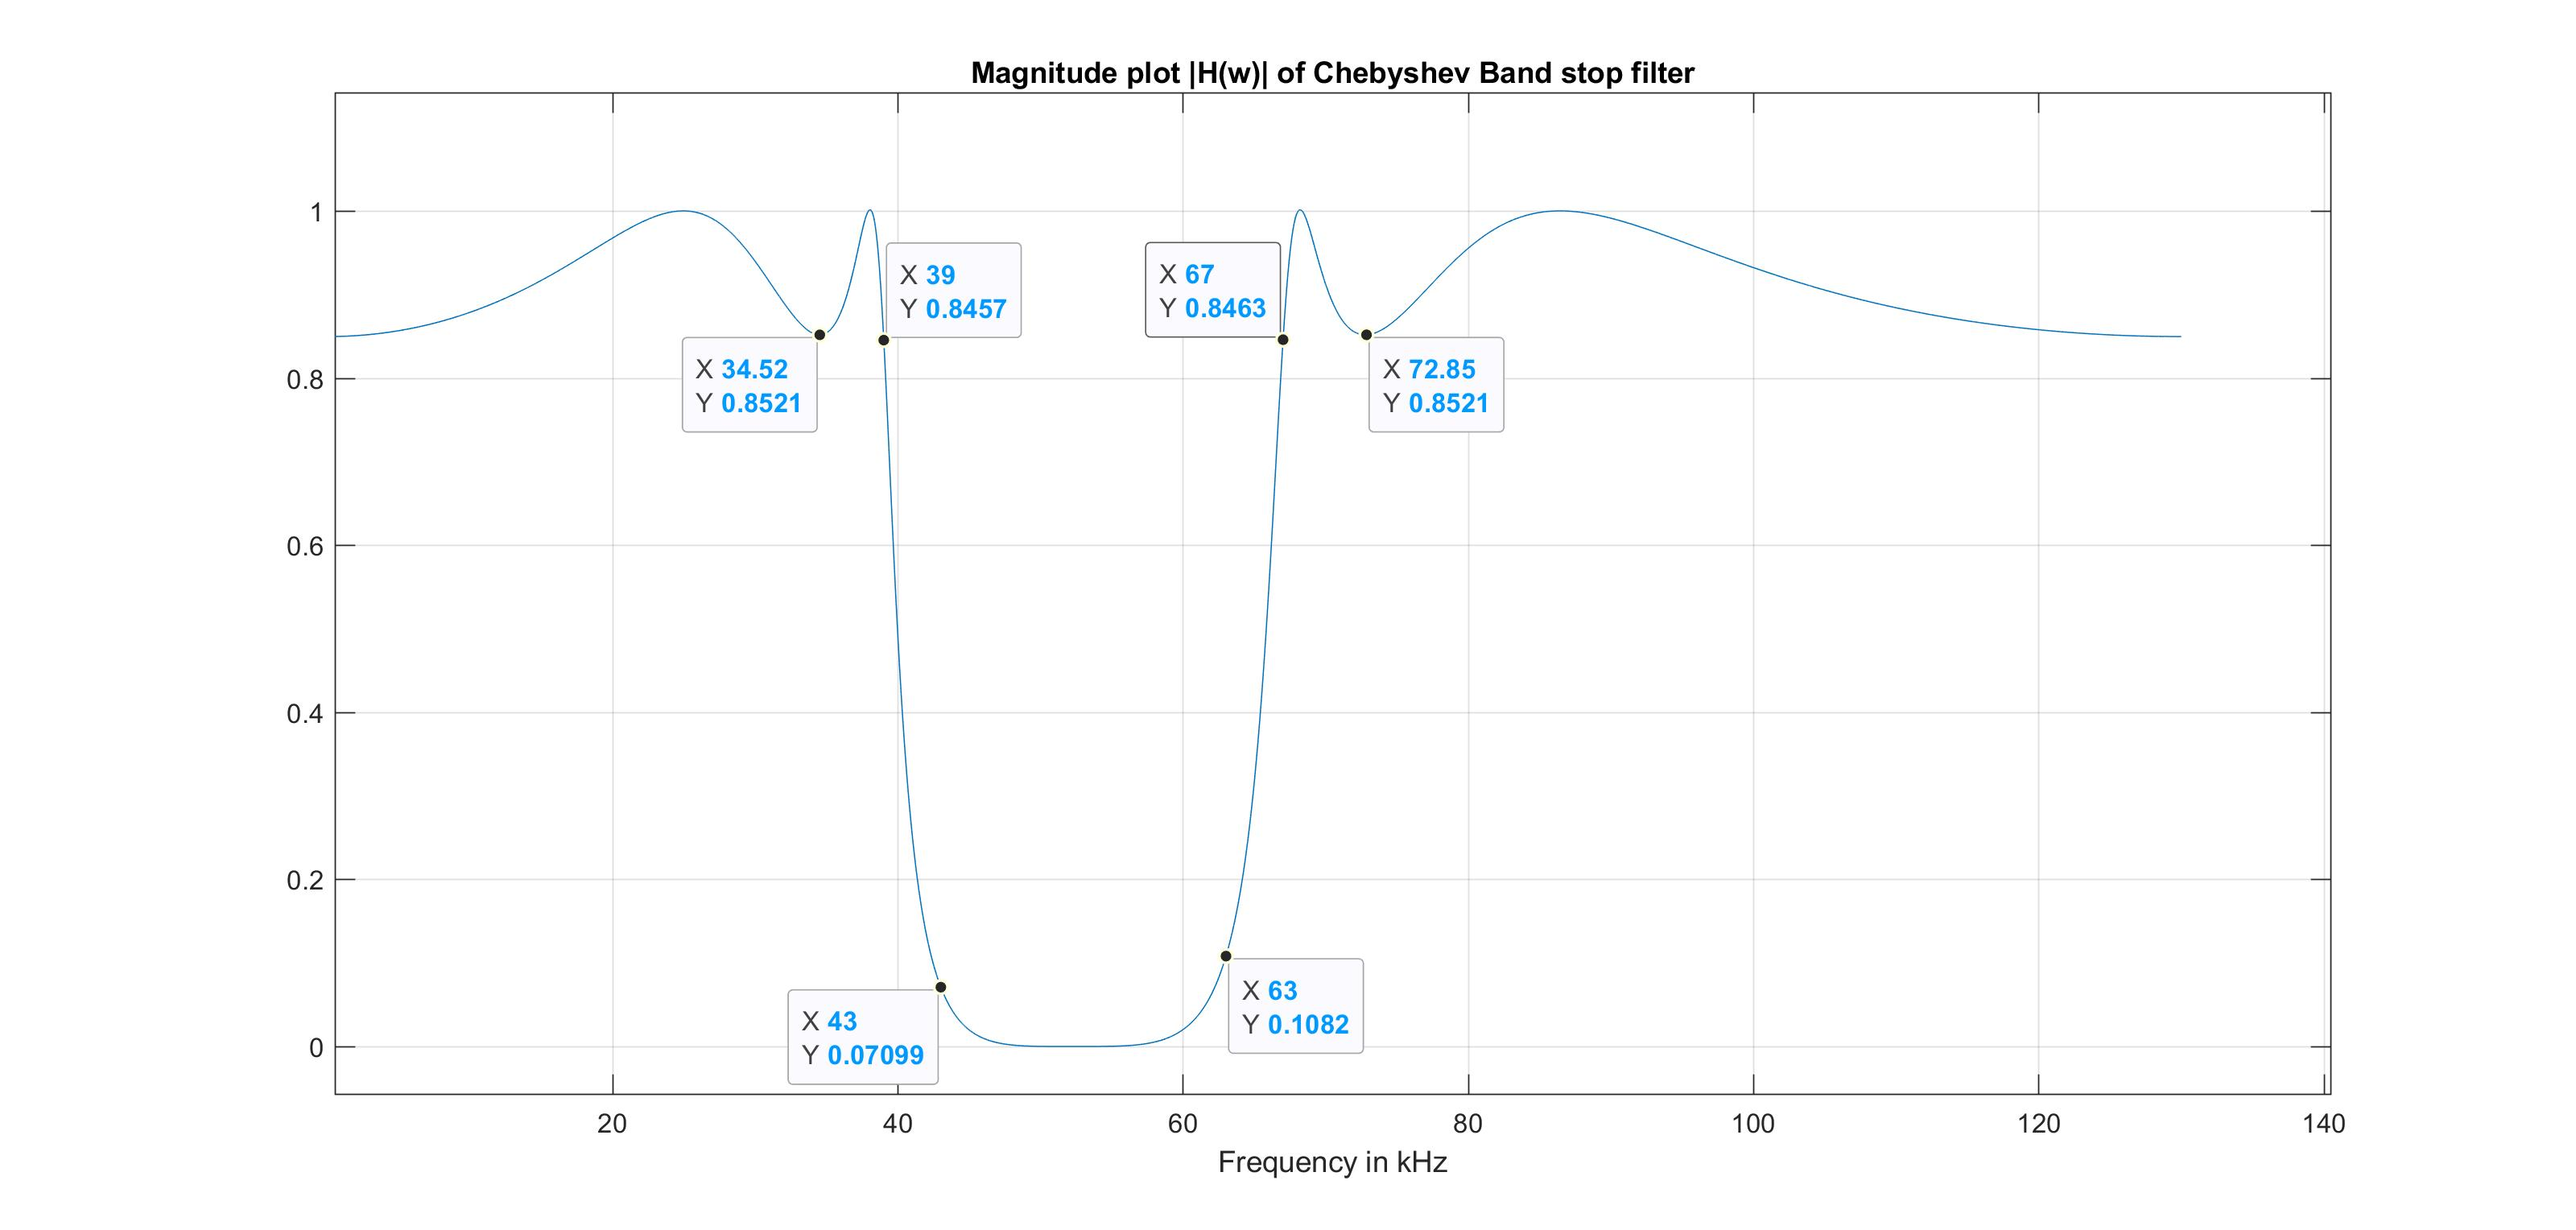
\includegraphics[width = 18cm, trim=0cm 0cm 0cm 0cm, clip]{Filter2DBSF.jpg}
	\end{figure}
	
\color{cyan}
\subsection{FIR Filter Transfer Function using Kaiser window}
\color{black}
Tolerance in both stop band and pass band is given to be 0.15. Therefore, $\delta$ = 0.15, using this we get value of A to be
\begin{gather*}
	A = -20*log(0.15) = 16.4782 dB
\end{gather*}
Since A$<$21, we get the value of the shape parameter of the Kaiser window $\alpha$ = 0. Hence we essentially get a rectangular window, Now the transition bandwidth $\Delta\omega_T$ = $\frac{4}{130} \pi \sim 0.03\pi$. Using the empirical formula for the length of the window,
\begin{gather*}
	2Nmin + 1 \ge 1 + \frac{A-8}{2.285\Delta\omega_T}
\end{gather*}
This gives us Nmin = 20, which implies the minimum length of the Kaiser window = 41. But this length does not satisfy all the conditions, the least window length satisfying all the conditions found by trial and error on MATLAB is n = 55.\\
We know the an Ideal Band Stop filter can be written as linear combination of three Ideal Low Pass Filters, So first we obtain the samples of the Ideal Band Stop filter by subtracting samples of two Low Pass filters and adding to another Low pass filter of same length as the Kaiser window. Now, we obtain the time domain representation of the final FIR filter by multiplying the Ideal impulse response samples with the Kaiser window.
\begin{figure}[H]
	\centering
	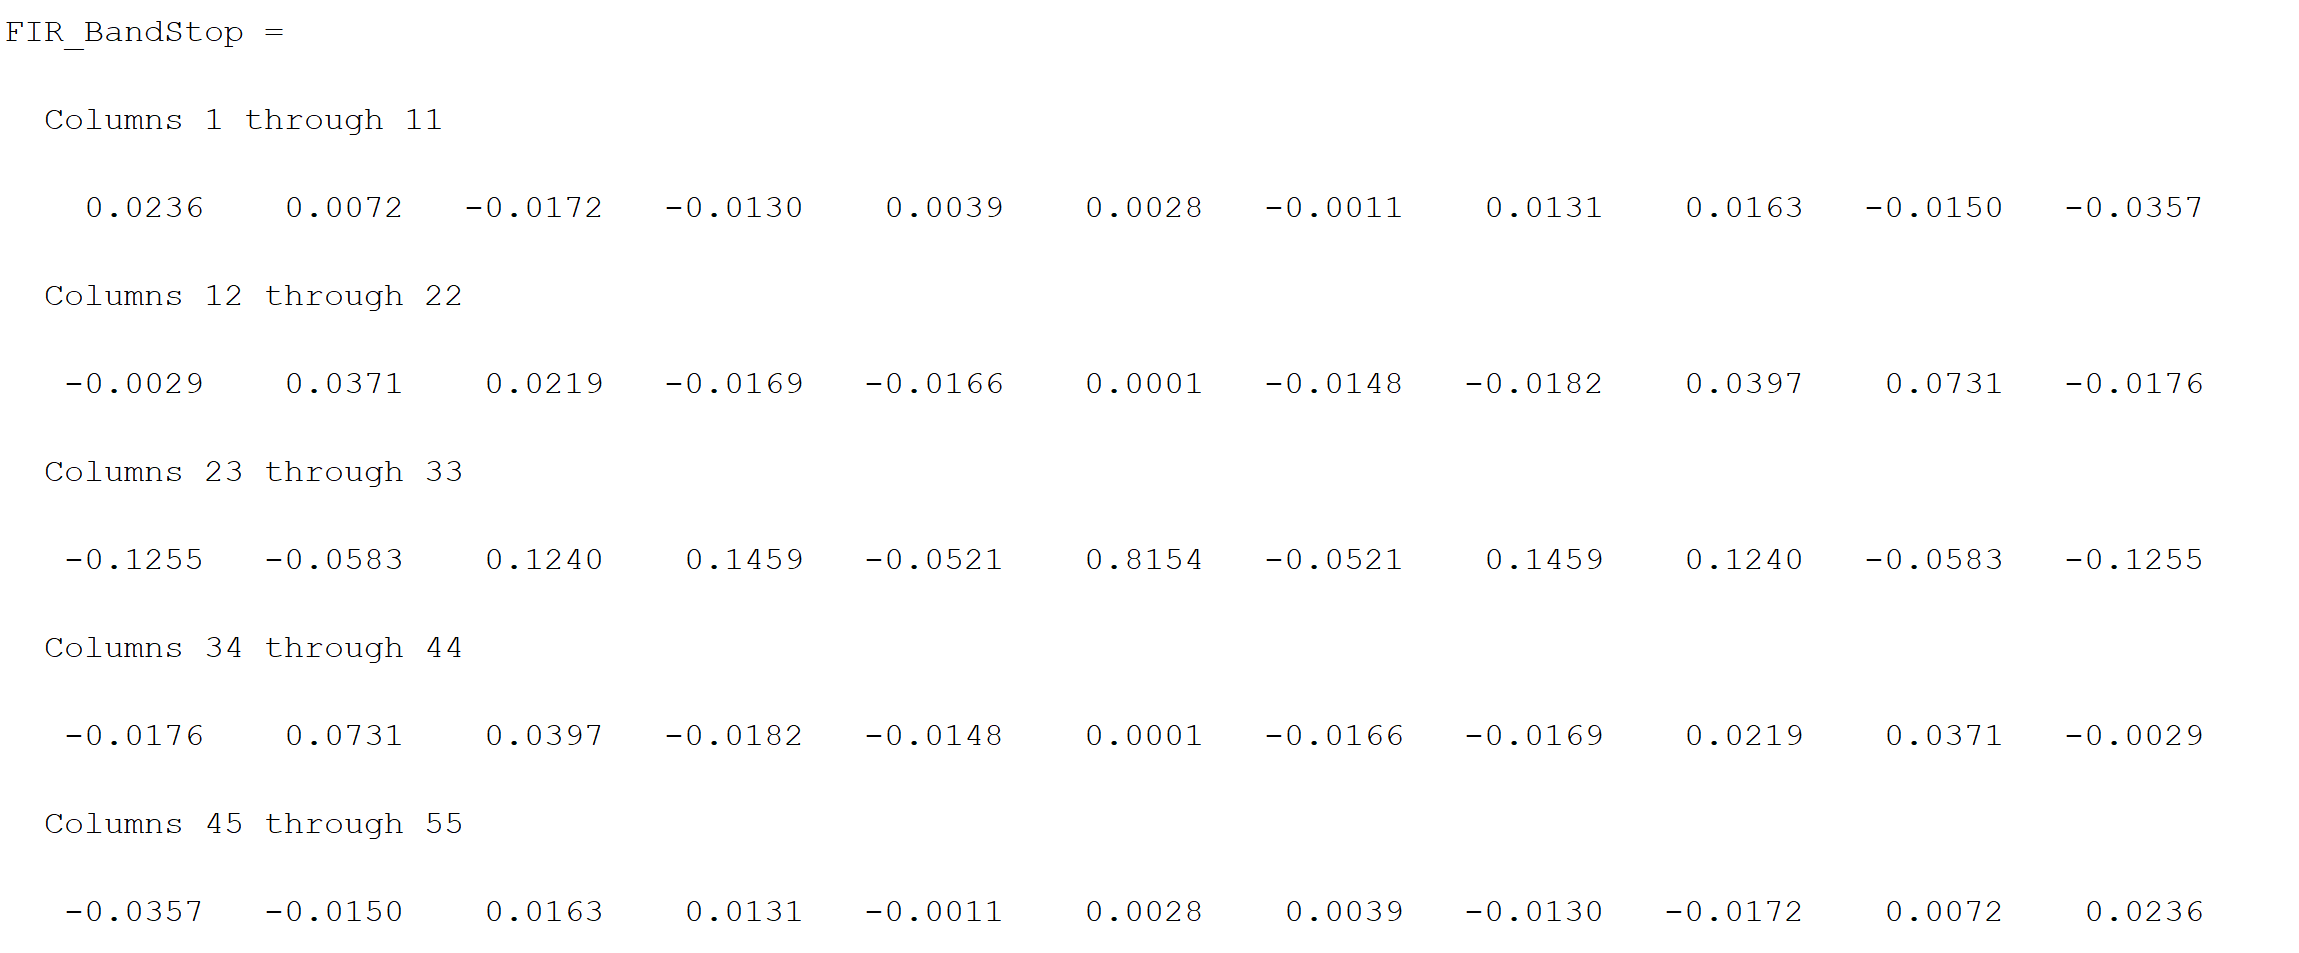
\includegraphics[width  = 18cm]{Filter2hn.png}
	\caption{Time Domain sequence values of the filter}
\end{figure}
\noindent These time domain sequence values are also the coefficients of the Z-transform from 1 to $Z^{-54}$.

\begin{figure}[H]
	\centering
	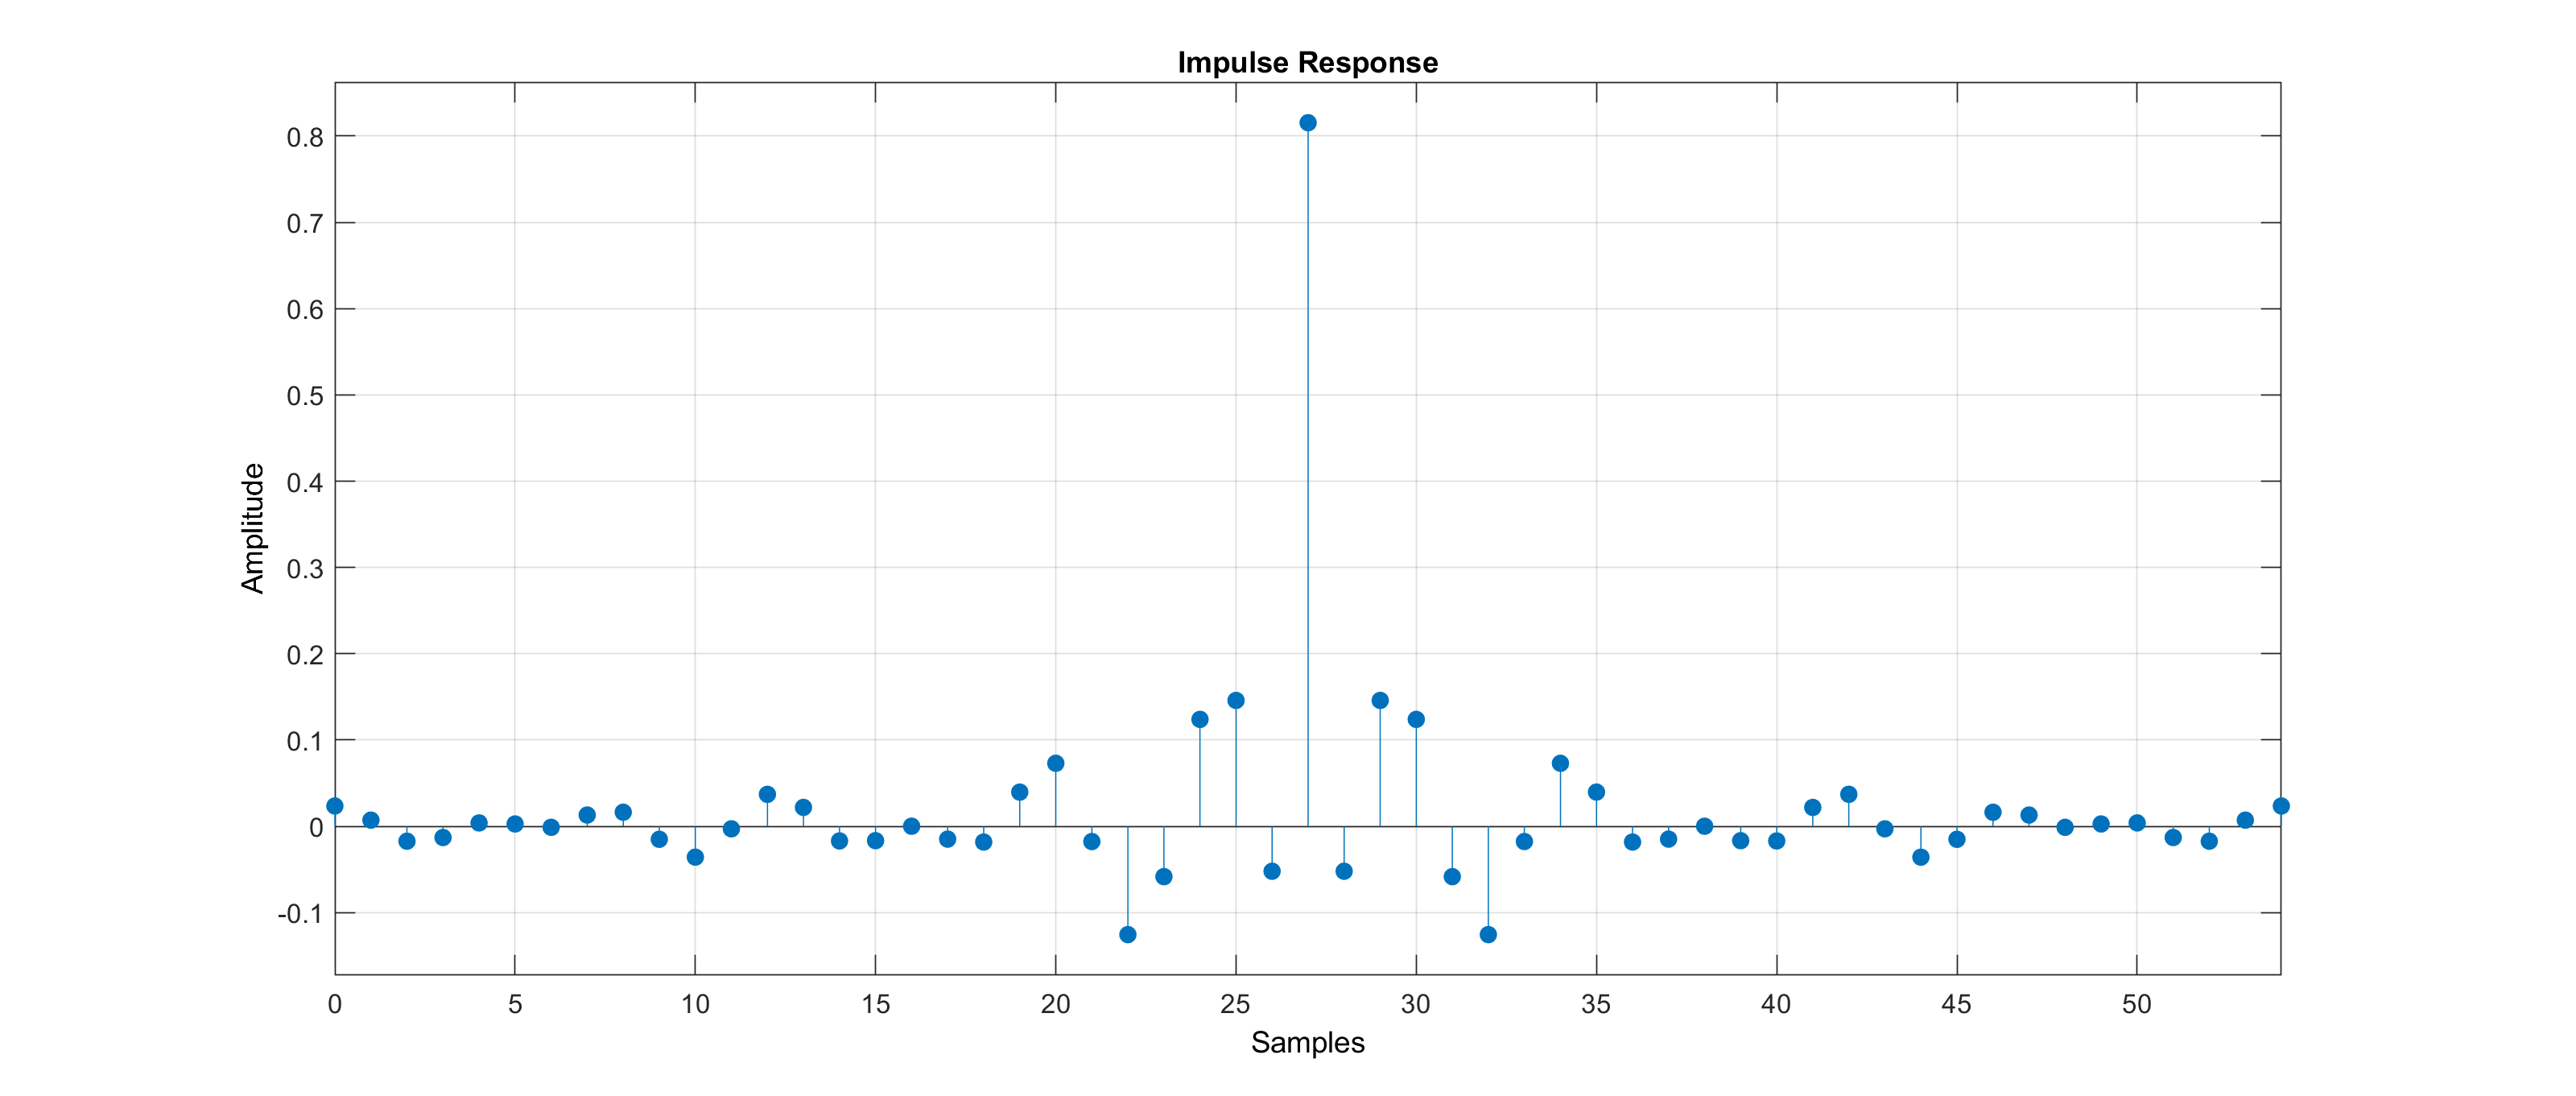
\includegraphics[width = 18cm]{FIRFilter2hn.png}
\end{figure}
\begin{figure}[H]
	\centering
	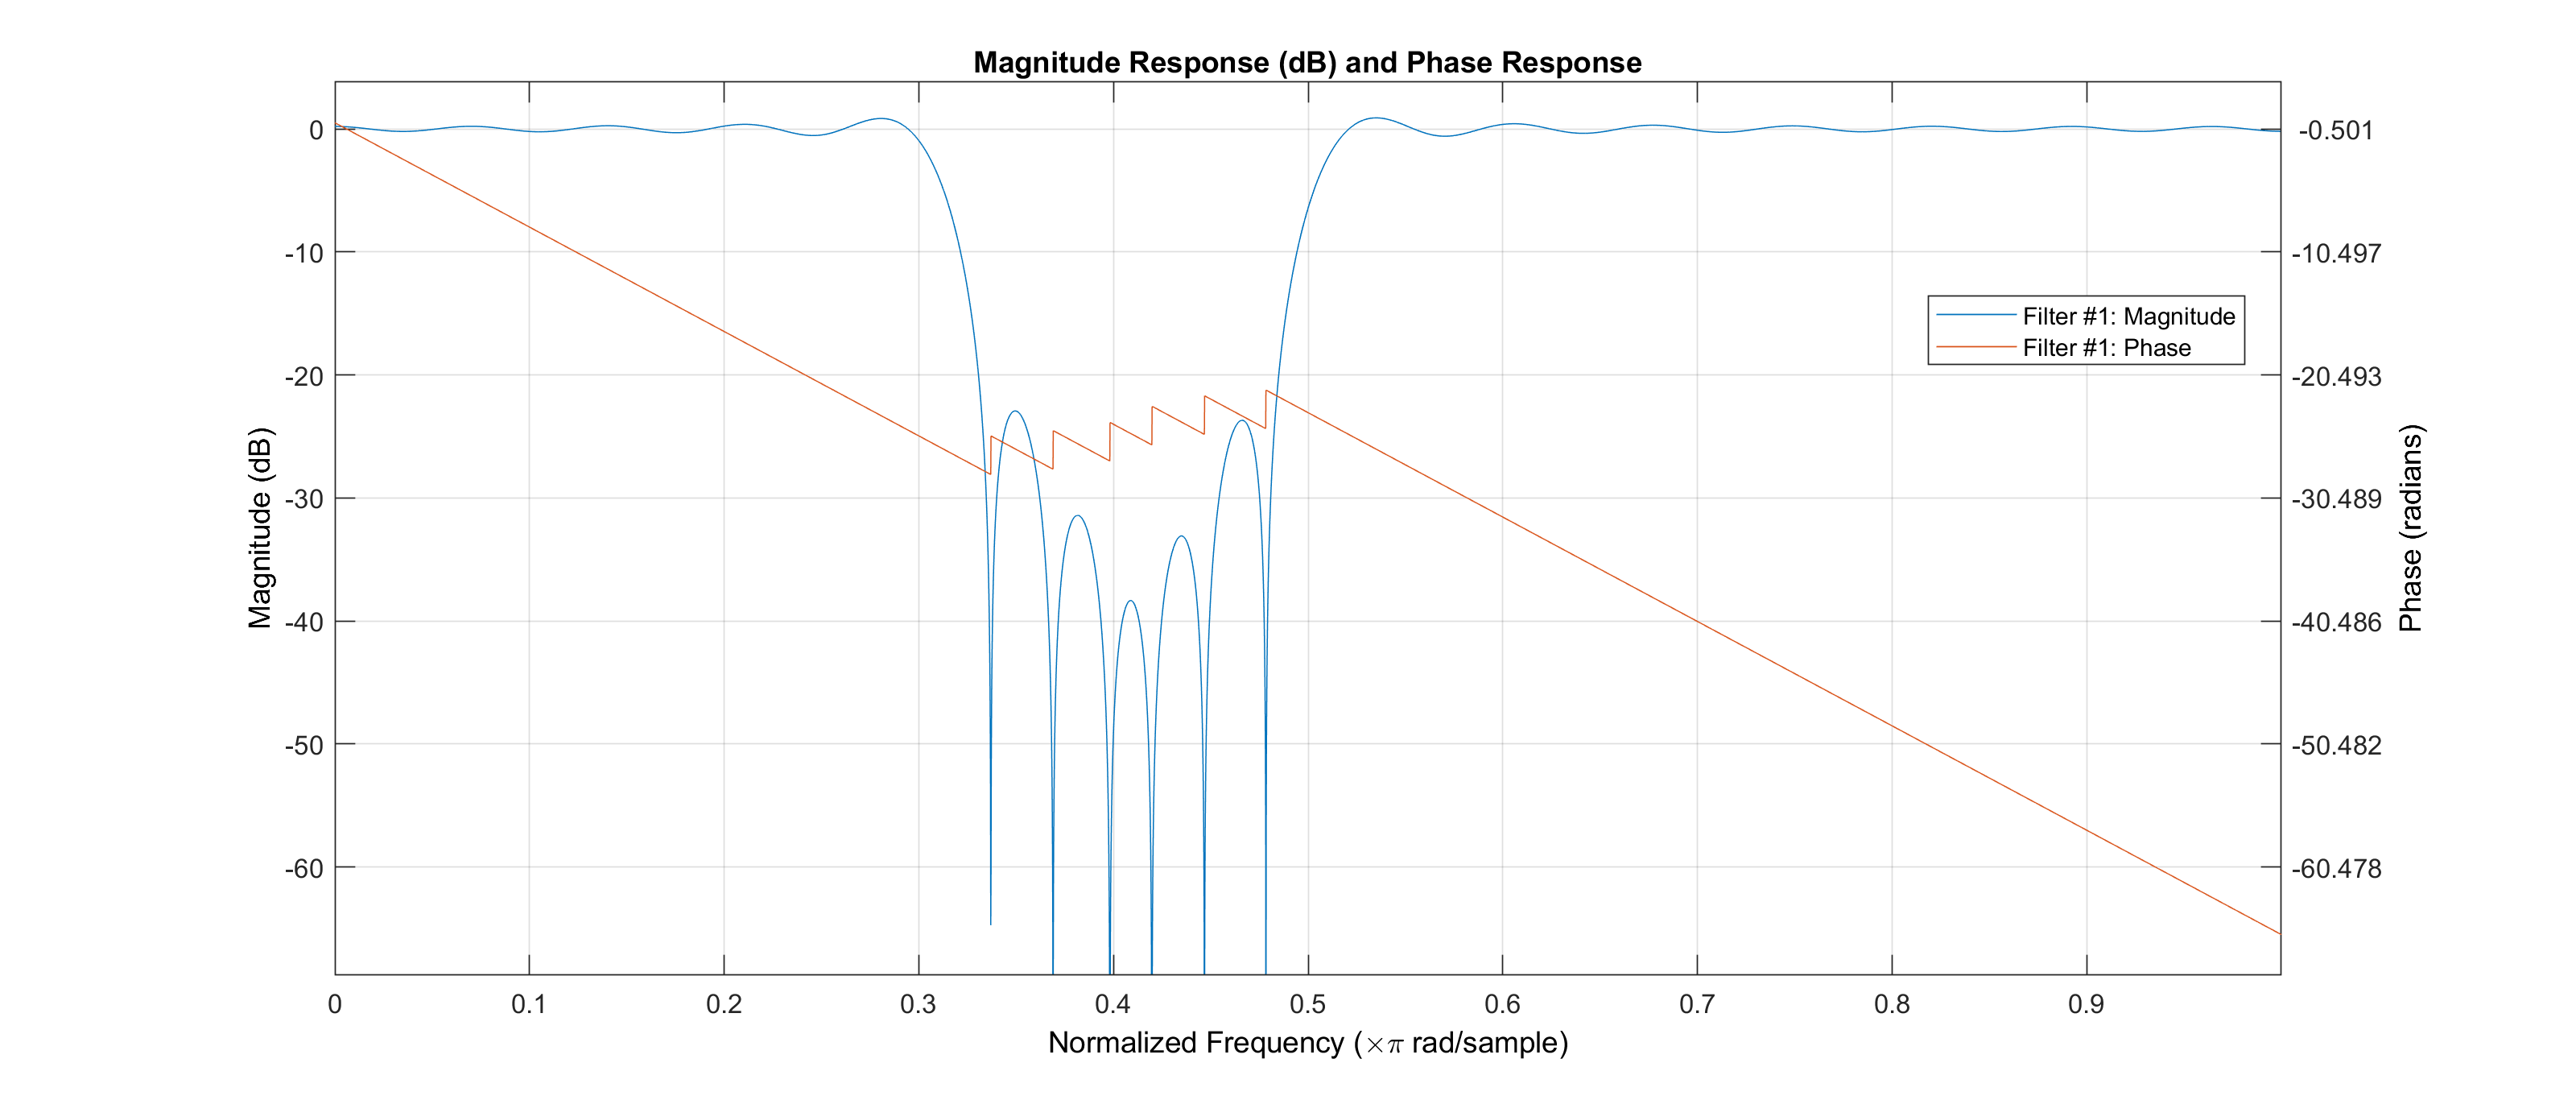
\includegraphics[width = 18cm, height = 10cm]{FIRFilter2MagPhase.png}
\end{figure}
\begin{figure}[H]
	\centering
	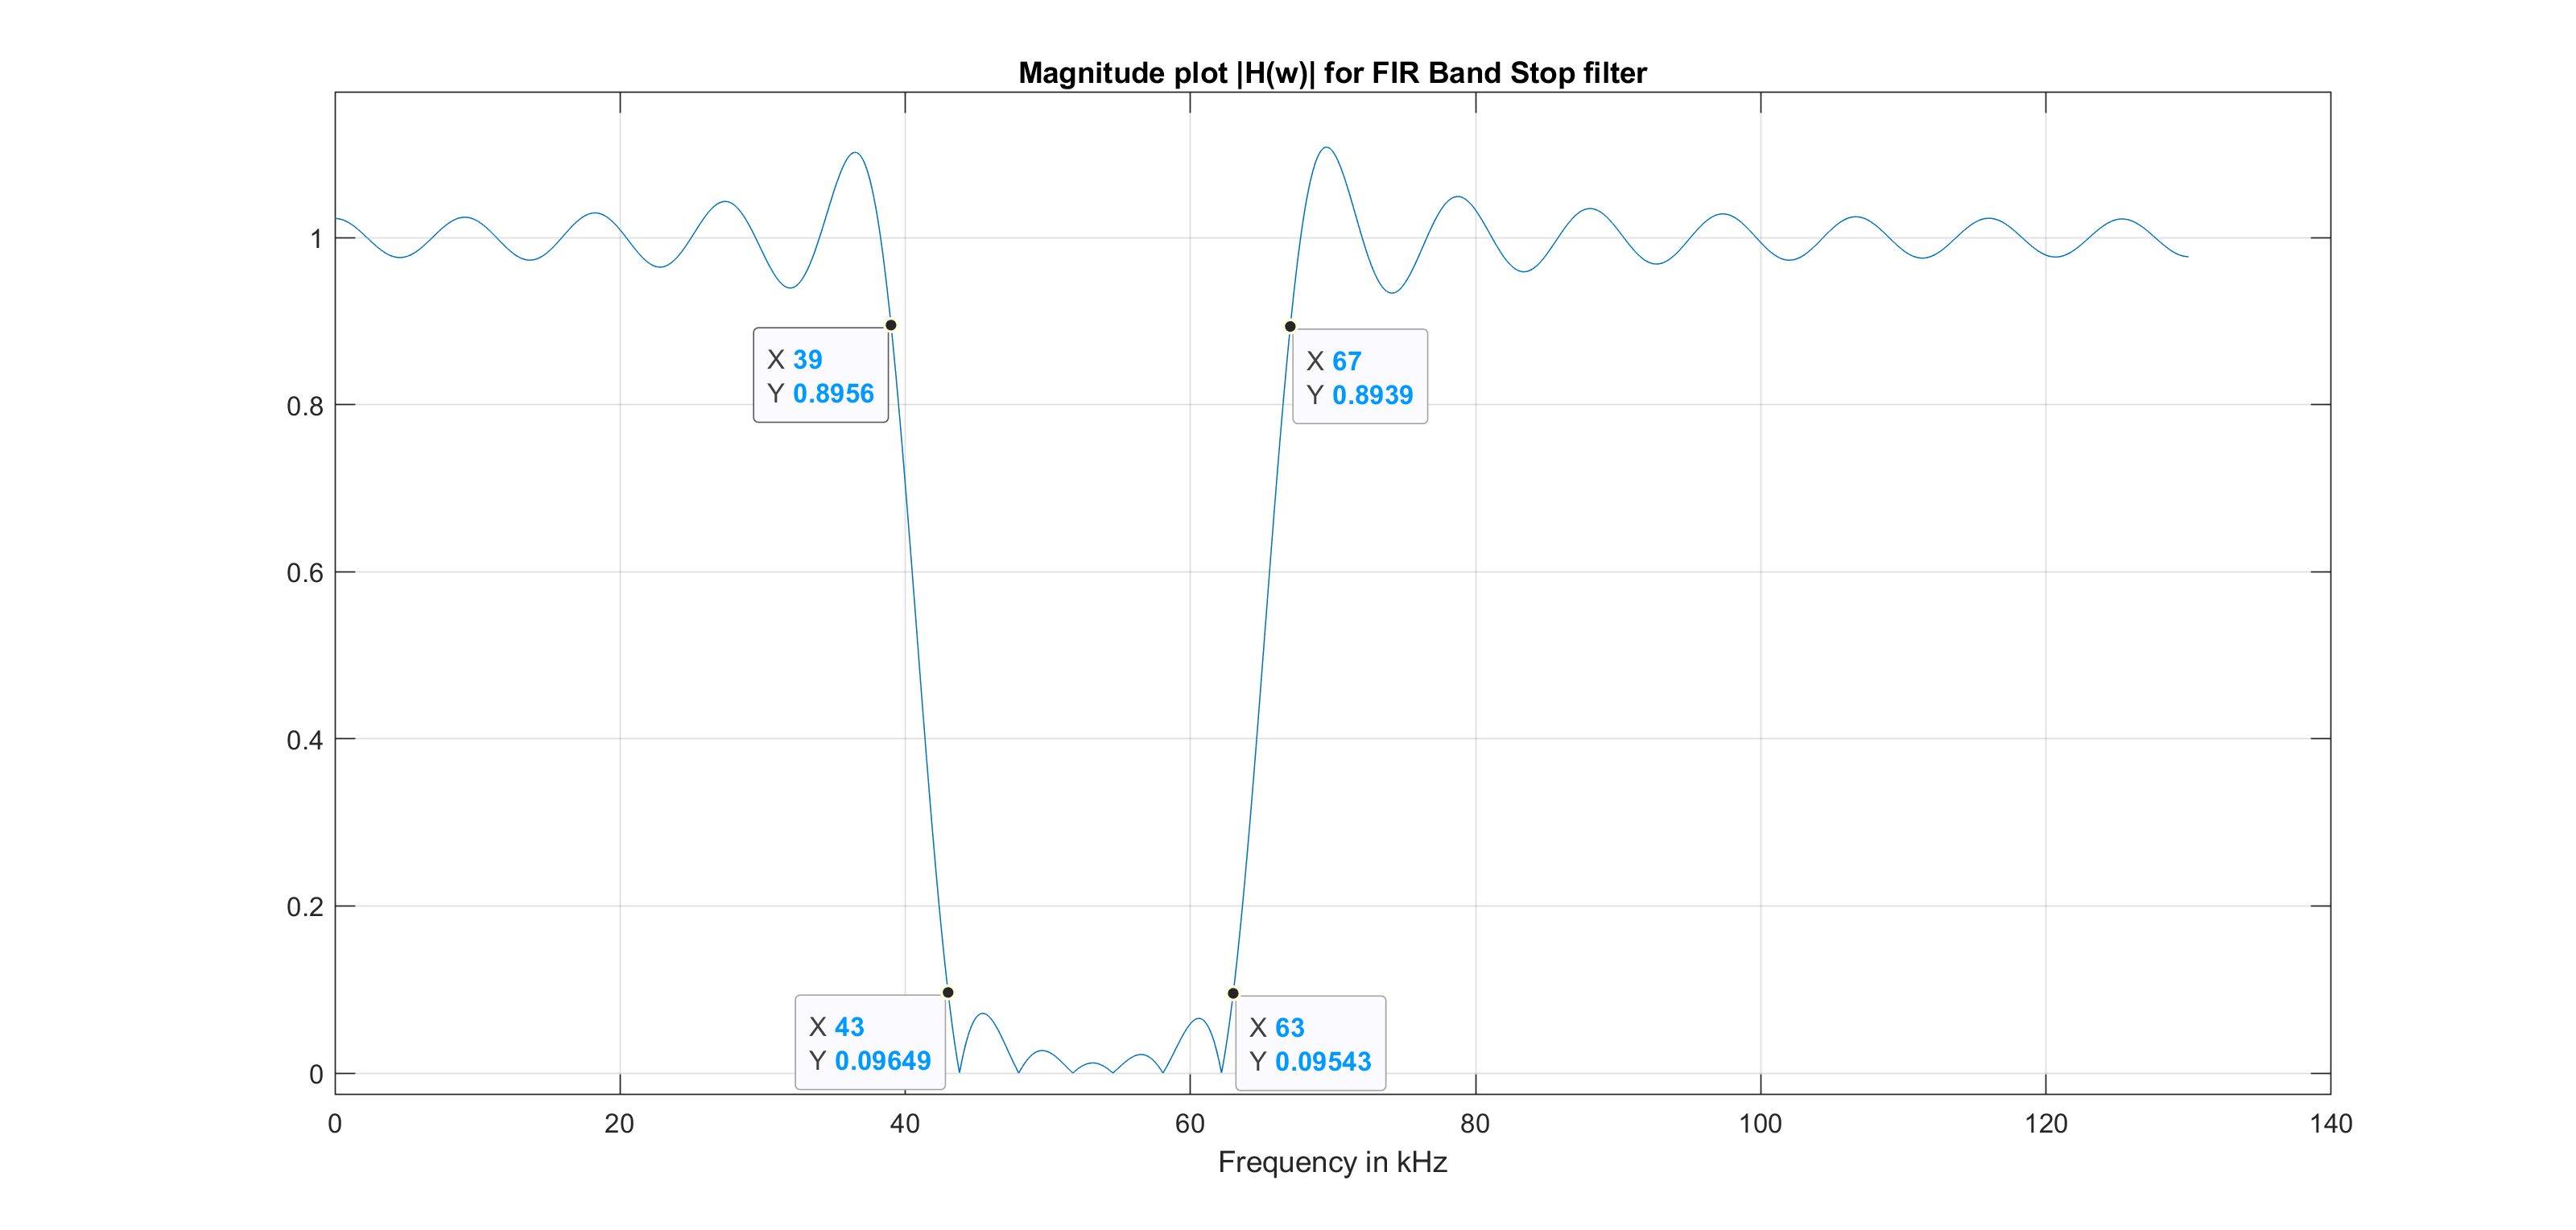
\includegraphics[width = 18cm]{FIRFilter2UBSF.png}
\end{figure}

\color{cyan}
\subsection{Comparison between FIR and IIR realizations}
\color{black}
\begin{itemize}
	\item As discussed in the class, we can see that the FIR filter has linear / Pseudo linear phase in the Pass band where as IIR filter has non-linear phase.
	\item The number of delay lines required for IIR filter is 8+8 = 16, where as for FIR filter we need 54 delay lines.  Hence it is very evident that for the same Filter specifications the FIR filters need a lot more hardware. 
\end{itemize}

\color{cyan}
\subsection{Review report}
\color{black}
Reviewed Shubham Kar's report
\begin{itemize}
	\item Specifications we correctly chosen but the formula written BL(m) was incorrect (but the final value was correct) and was now modified.
	\item All the frequency response specifications are met. We can see this clearly as he marked the critical points on the plots.
	\item All the mandatory parts are done. Although there were some typo's which were corrected.
\end{itemize}
\newpage

\color{darkblue}
\noindent\textbf{\Large{Part2: Elliptic Filters}}
\section{Filter 1: Elliptic Band Pass Filter}
\color{black}
Since all the specification except the Stop band and Pass Band Nature are same, the same analysis will be done until specifying the Low pass filter Transfer function as we have done for Filter 1. \begin{itemize}
	\item Filter Number Assigned = m = 33
	\item Both Pass band and Stop band tolerances are 0.15
	\item Pass band: Equiripple 
	\item Stop band: Equiripple
	\item Elliptic / Jacobi Approximation
	\item Band-Pass filter.
	\item The Transition band is 4kHz on either side of the pass band
	\item The input signal is Band limitted to 160kHz and the sampling rate is 330kHz.
\end{itemize}
\color{cyan}
\subsection{Unnormalized Specifications}
\color{black}
m = 33\\
q(m) = 3\\
r(m) = 33 - 30 = 3\\
BL(m) = 25 + 1.7 $\times$ 3 + 6.1 $\times$ 3 = 48.4 kHz\\
BH(m) = BL(m) + 20 = 68.4 kHz\\

\noindent Hence the filter specifications for the Bandpass Filter are:
\begin{itemize}
	\item Pass band is 48.4 kHz to 68.4 kHz
	\item Transition band is 4kHz on either side of the Pass band
	\item Stop band is 0 to 44.4 kHz and 72.4 kHz to 165 kHz
	\item Tolerances for both bands are 0.15
	\item Both Pass band and Stop band are Equiripple
\end{itemize}

\color{cyan}
\subsection{Normalized specifications}
\color{black}
Given sampling rate  = 330 kHz. Using\\
\begin{gather*}
	\omega = \frac{2\pi \ast \Omega}{\Omega_s}
\end{gather*}
where $\omega$ is the normalized frequency, $\Omega$ is the Un-normalized frequency and $\Omega_s$ is the sampling frequency.
\begin{itemize}
	\item Pass band is $\frac{22}{75}\pi$ to $\frac{114}{275}\pi$ $\sim$ (0.29$\pi$ to 0.415$\pi$)
	\item Transition band is $\frac{4}{165}\pi$ $\sim$ (0.024$\pi$) on either side of the Pass band
	\item Stop band is 0 to  $\frac{74}{275}\pi$ and $\frac{362}{825}\pi$ to $\pi$  $\sim$(0 to 0.27$\pi$ and  0.44$\pi$ to $\pi$)
	\item Tolerances for both bands are 0.15
	\item Both Pass band and Stop band are Equiripple
\end{itemize}

\color{cyan}
\subsection{Analog Band-pass Filter Specifications}
\color{black}
Using Bilinear Transformation,
\begin{gather*}
	\Omega = tan\left(\frac{\omega}{2}\right)
\end{gather*}
where $\Omega$ is the analog domain frequency and $\omega$ is the discrete domain frequency\\

\begin{center}
	\begin{tabular}{ |c|c|c|c|c|c|c| }
		\hline
		&&&&&&\\
		Domain& Zero & $\Omega_{S1}$ & $\Omega_{P1}$ &$\Omega_{P2}$& $\Omega_{S2}$&Infinity\\
		&&&&&&\\
		\hline
		&&&&&&\\
		$\omega$ & 0 & $\frac{74}{275}\pi$ & $\frac{22}{75}\pi$& $\frac{114}{275}\pi$& $\frac{362}{825}\pi$& $\pi$\\
		&&&&&&\\
		\hline
		&&&&&&\\
		$\Omega$ & 0 & 0.45 & 0.496 & 0.762& 0.824 & $\infty$\\
		&&&&&&\\
		\hline
	\end{tabular}
\end{center}

\noindent Hence the filter specifications for the corresponding analog domain Bandpass Filter are:
\begin{itemize}
	\item Pass band is 0.496 ($\Omega_{P1}$)  to 0.762 ($\Omega_{P2}$) 
	\item Stop band is 0 to 0.45($\Omega_{S1}$) and 0.824 ($\Omega_{S2}$) to $\infty$
	\item Tolerances for both bands are 0.15
	\item Both Pass band and Stop band are Equiripple
\end{itemize}

\color{cyan}
\subsection{Frequency Transformation in to a Low Pass Filter}
\color{black}
Using the Band-Pass Transformation
\begin{gather*}
	\Omega_L = \frac{\Omega^2 - \Omega_0^2}{B\Omega}\\\\
	\Omega_0 = \sqrt{\Omega_{P1} \Omega_{P2}} = 0.615\\\\
	B = \Omega_{P2} - \Omega_{P1} = 0.2656
\end{gather*}

\begin{center}
	\begin{tabular}{ |c|c|c|c|c|c|c|c| }
		\hline
		&&&&&&&\\
		Domain &Zero & $\Omega_{S1}$ & $\Omega_{P1}$ &$\Omega_0$ &$\Omega_{P2}$& $\Omega_{S2}$ &Infinity\\
		&&&&&&&\\
		\hline
		&&&&&&&\\
		$\Omega$ & 0$^+$ & 0.45 & 0.496 &0.615 &0.762& 0.824 & $\infty$\\
		&&&&&&&\\
		\hline
		&&&&&&&\\
		$\Omega_L$ & -$\infty$ & -1.4727 & -1 & 0 &1 & 1.3741 & $\infty$\\
		&&&&&&&\\
		\hline
		&&&&&&&\\
		Domain& -Infinity & $\Omega_{LS1}$ & $\Omega_{LP1}$ &$\Omega_0$ &$\Omega_{LP2}$& $\Omega_{LS2}$ &Infinity\\
		&&&&&&&\\
		\hline
	\end{tabular}
\end{center}
 
\color{cyan}
\subsection{Analog Low Pass Filter Specifications}
\color{black}
\begin{itemize}
	\item Pass band edge is at 1 ($\Omega_{LP}$)
	\item Stop band edge = min (-$\Omega_{LS1}$, $\Omega_{LS2}$) = 1.3741 ($\Omega_{LS}$)
	\item Tolerances = $\delta_1$ = $\delta_2$ = 0.15 for both Stop band and Pass band
	\item Both Pass band and Stop band are Equiripple
\end{itemize}

\color{cyan}
\subsection{Analog Low Pass Filter Transfer function}
\color{black}
The magnitude-squared frequency response of an elliptic filter is defined as
\begin{gather*}
	H_{analog,LPF}^2(j\Omega) = \frac{1}{1+\epsilon^2R_{n}^2(\Omega, \Omega_{LS}, \delta_1, \delta_2)}
\end{gather*}
Where $R_n$ is the nth-order elliptic rational function also known as a Chebyshev rational function. The order n, $\epsilon$ and will depend on the required specifications.
The minimum order required can be calculated using the following steps,
\begin{gather*}
\delta_1 = \delta_2 = 0.15\\
D_1 = \frac{1}{(1-\delta_1)^2} - 1 = 0.3841\\
D_2 = \frac{1}{\delta_2^2} - 1 = 43.4444\\
\epsilon = \sqrt{D1} = 0.61975\\
k = \frac{\Omega_{LP}}{\Omega_{LS}} =  \frac{1}{1.3741} = 0.72775\\
k' = \sqrt{1-k^2} = 0.6858\\
k_1 = \sqrt{\frac{D1}{D2}} = 0.094\\
k_1' = \sqrt{1-k_1^2} = 0.99557\\
Nmin \ge \frac{KK_1'}{K'K_1}
\end{gather*}
Where K, K', $K_1$, $K_1'$ are the values of complete elliptic integrals evaluated at k, k', $k_1$, $k_1'$.\\
We get, K = 1.88 , K' = 1.8298, $K_1$ = 1.5743, $K_1'$ = 3.7566. Using these values, we get the order of the elliptic rational function as 3. Once we get $N_{min}$, we need to recompute k and $\Omega_{LS}$ for all the conditions to be satisfied.
\begin{gather*}
	Nmin = \ceil{2.451} = 3 
\end{gather*}
Where, Elliptic integral is defined as,
\begin{gather*}
	u(\phi,k) = \int_{0}^{\phi} \frac{dy}{\sqrt{1-k^2sin^2(y)}}
\end{gather*} 
and complete elliptic integral is equal to u($\pi$/2, k). i.e,
\begin{gather*}
	U(k) = \int_{0}^{\pi/2} \frac{dy}{\sqrt{1-k^2sin^2(y)}}
\end{gather*}
Using the above elliptic integral equation we can also write $\phi$ in terms of $u$,k. i.e, $\phi(u$,k). This is the inverse of elliptic integral function. Using this we can define Jacobi elliptic sine function and other elliptic functions are defined as,
\begin{gather*}
	sn(u,k) = sin(\phi(u,k))\\
	cn(u,k) = cos(\phi(u,k))\\
	dn(u,k) = \sqrt{1-k^2sn^2(u,k)}\\
	cd(u,k) = \frac{cn(u,k)}{dn(u,k)}
\end{gather*}
The Chebyshev rational function can be represented as,
\begin{gather*}
	R_n(\Omega) = sn(N_{min}\times sn^{-1}(\Omega,k),k_1)\\
	R_n(\Omega) = sn(\phi,k_1), \Omega = sn(\phi,k)
\end{gather*}
The zero locations of the Transfer function can be given by,
\begin{gather*}
	\Omega = \frac{\pm1}{k cd(iK/N_{min},k)}, i.e.,\\
	s = \frac{\pm j}{k cd(iK/N_{min},k)}
\end{gather*}
Where i = 0, 2, 4, ..., N-1 for Odd N, and i = 1, 3, 5, ... N-1 for Even N.\\
The pole locations of the transfer function can be given by,
\begin{gather*}
	 1 + \epsilon^2R_n(s/j)^2 = 0
\end{gather*}
Using the periodicity of sn(u,k), we get
\begin{gather*}
	sn(N_{min}\phi, + 2K_1i,k_1) = \pm j\frac{1}{\epsilon}\\
	\phi = (-2Ki + sn^{-1}(\frac{j}{\epsilon},k_1))/N_{min}\\
	\Omega = sn(\phi,k)
\end{gather*}

\noindent Define, 
\begin{gather*}
	jV_0 = sn^{-1}(\frac{j}{\epsilon},k_1)/N_{min}
\end{gather*}

Using these equations, location of poles can be found using
\begin{gather*}
s = j sn(Ki/N + jV_0,k) = jcd(Ki/N + (1-jV_0),k)
\end{gather*}
Note that here j represents complex number and i = 0, 2, 4, ..., N-1 for Odd N, and i = 1, 3, 5, ... N-1 for Even N.
From the above equations, the poles and zeroes are found to be:
\begin{verbatim}
	
	p1=-0.11533-0.9936i
	p2=-0.11533+0.9936i
	p3=-0.6232
	z1=-1.2604i
	z2=1.2604i 
\end{verbatim}
Using these poles and zeroes the transfer function Low pass analog filter is given by,

\begin{gather*}
	H_{analog,LPF}(s_{L}) = \frac{0.3925s_L^2 + 0.6235}{s_L^3 + 0.8538s_L^2 + 1.1443s_L + 0.6235}	
\end{gather*}

\begin{figure}[H]
	\centering
	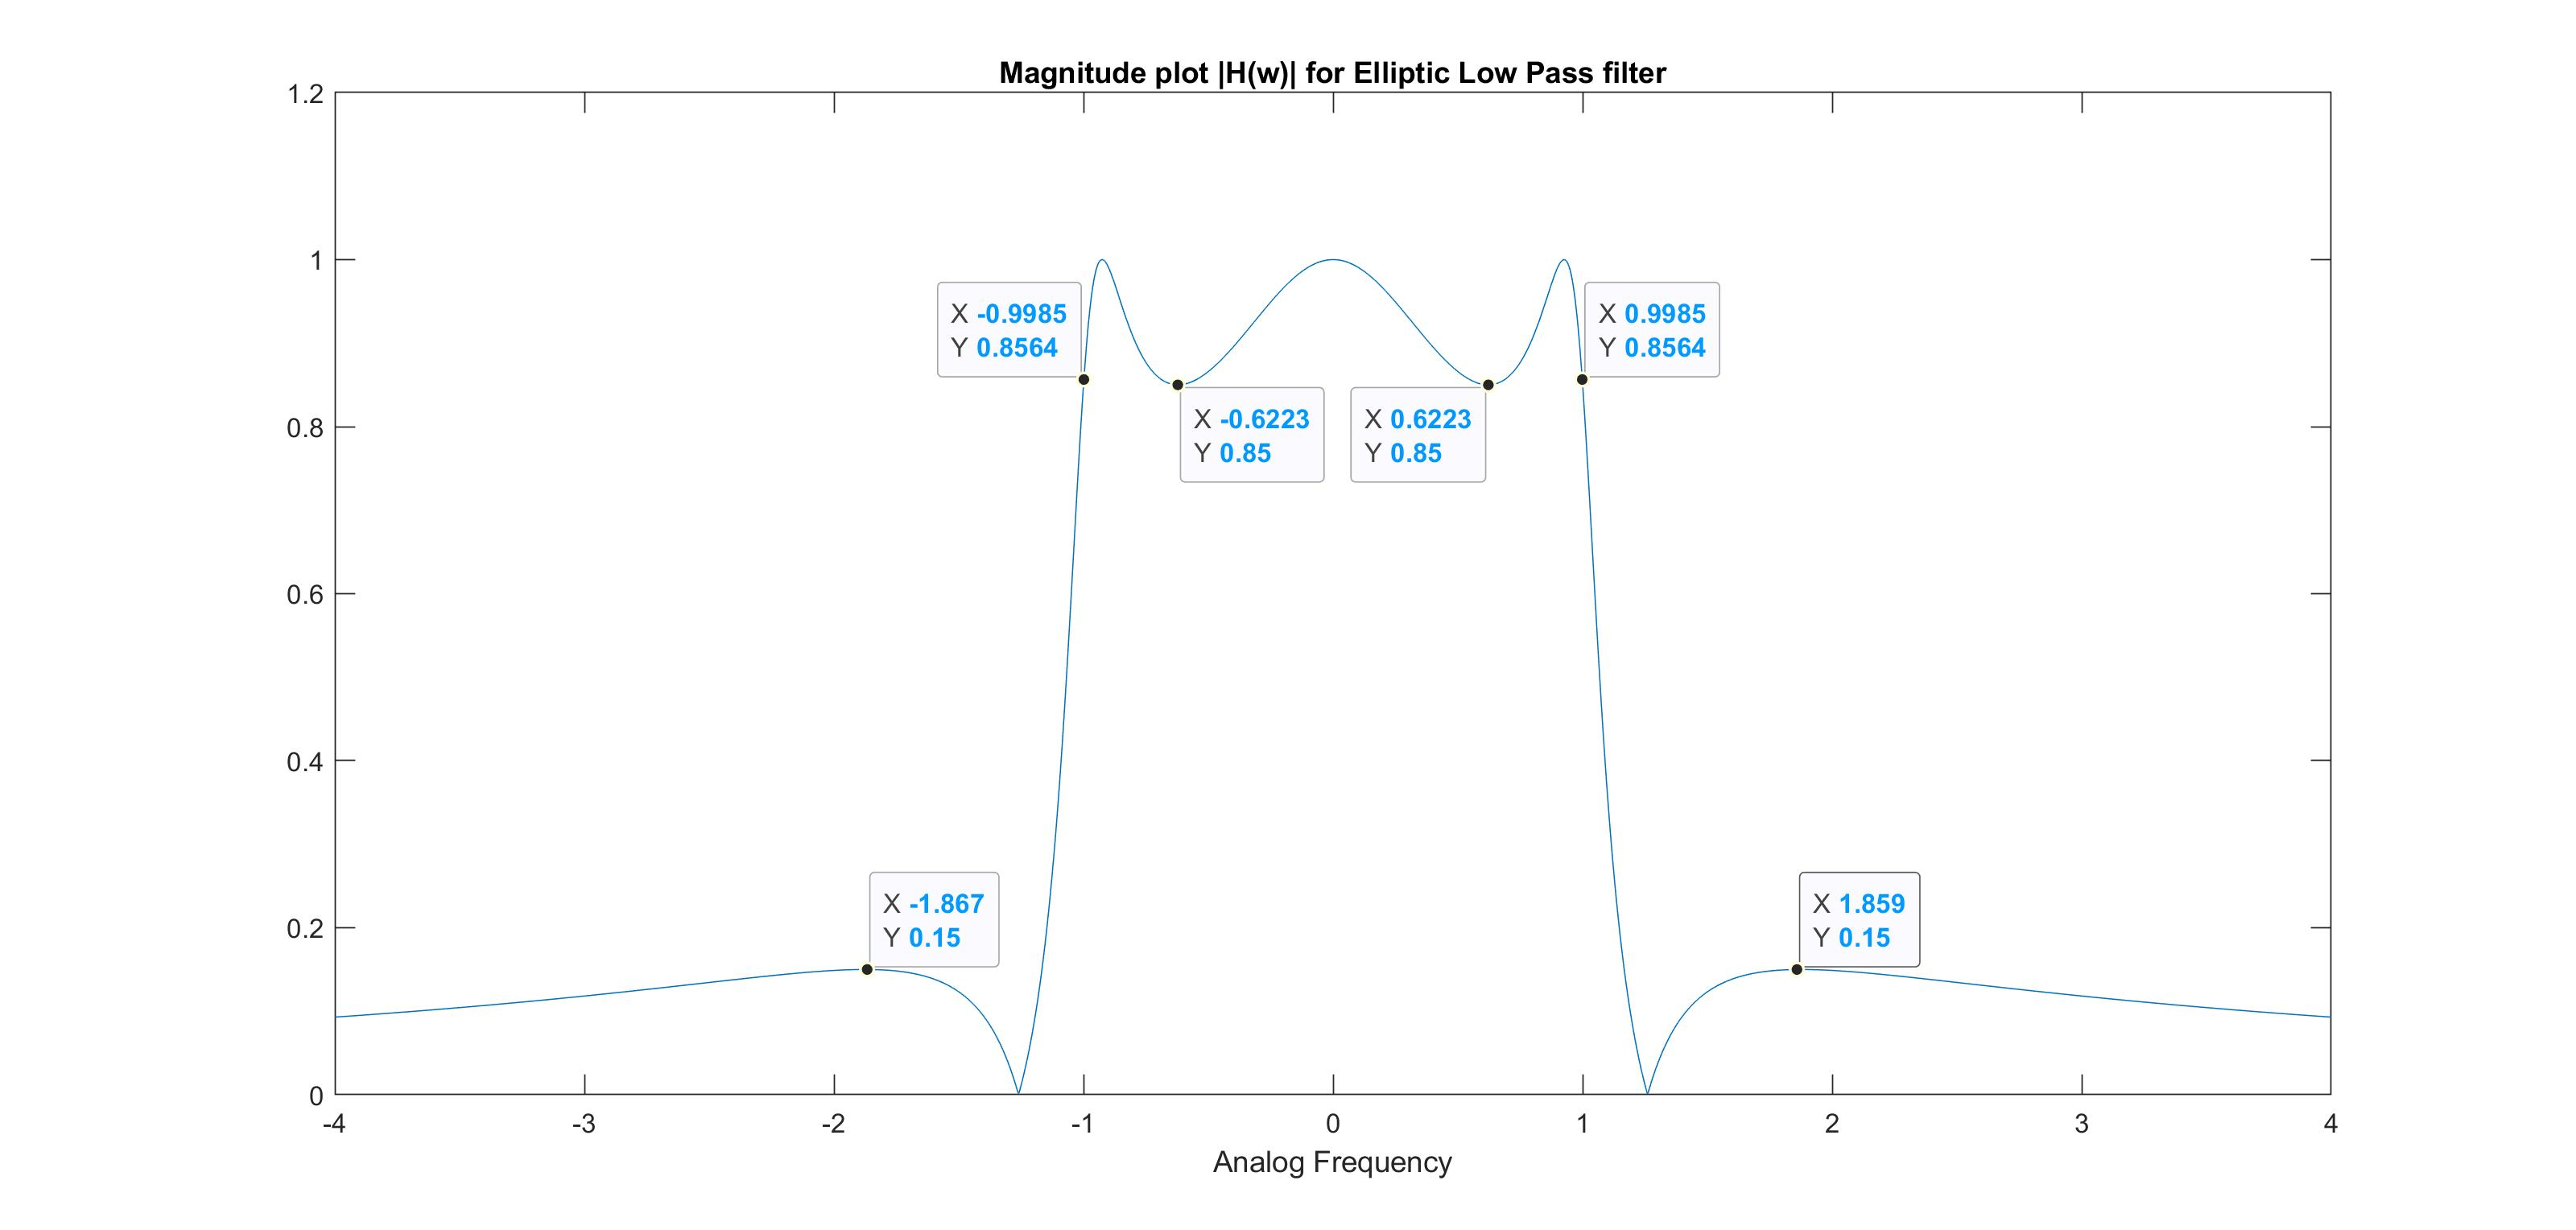
\includegraphics[width = 18cm]{Filter3ALPF.jpg}
\end{figure}

\color{cyan}
\subsection{Analog Band Pass Transfer function}
\color{black}

Using the Band pass transformation:
\begin{gather*}
	s_L = \frac{s^2 + \Omega_0^2}{Bs}
\end{gather*}
Substituting the values B = 0.266 and $\Omega_0$ = 0.615,
\begin{gather*}
	s_L = \frac{s^2 + 0.378}{0.266s}
\end{gather*}
Substituting this back into $H_{analog,LPF}$, we get $H_{analog,BPF}$ as
\begin{gather*}
	\frac{0.1043s^5 +0.0906s^3 + 0.0149s}{s^6 + 0.2268s^5 + 1.2156s^4 + 0.1833s^3 + 0.4598s^2 + 0.0325s + 0.0541}	
\end{gather*}
\begin{figure}[H]
	\centering
	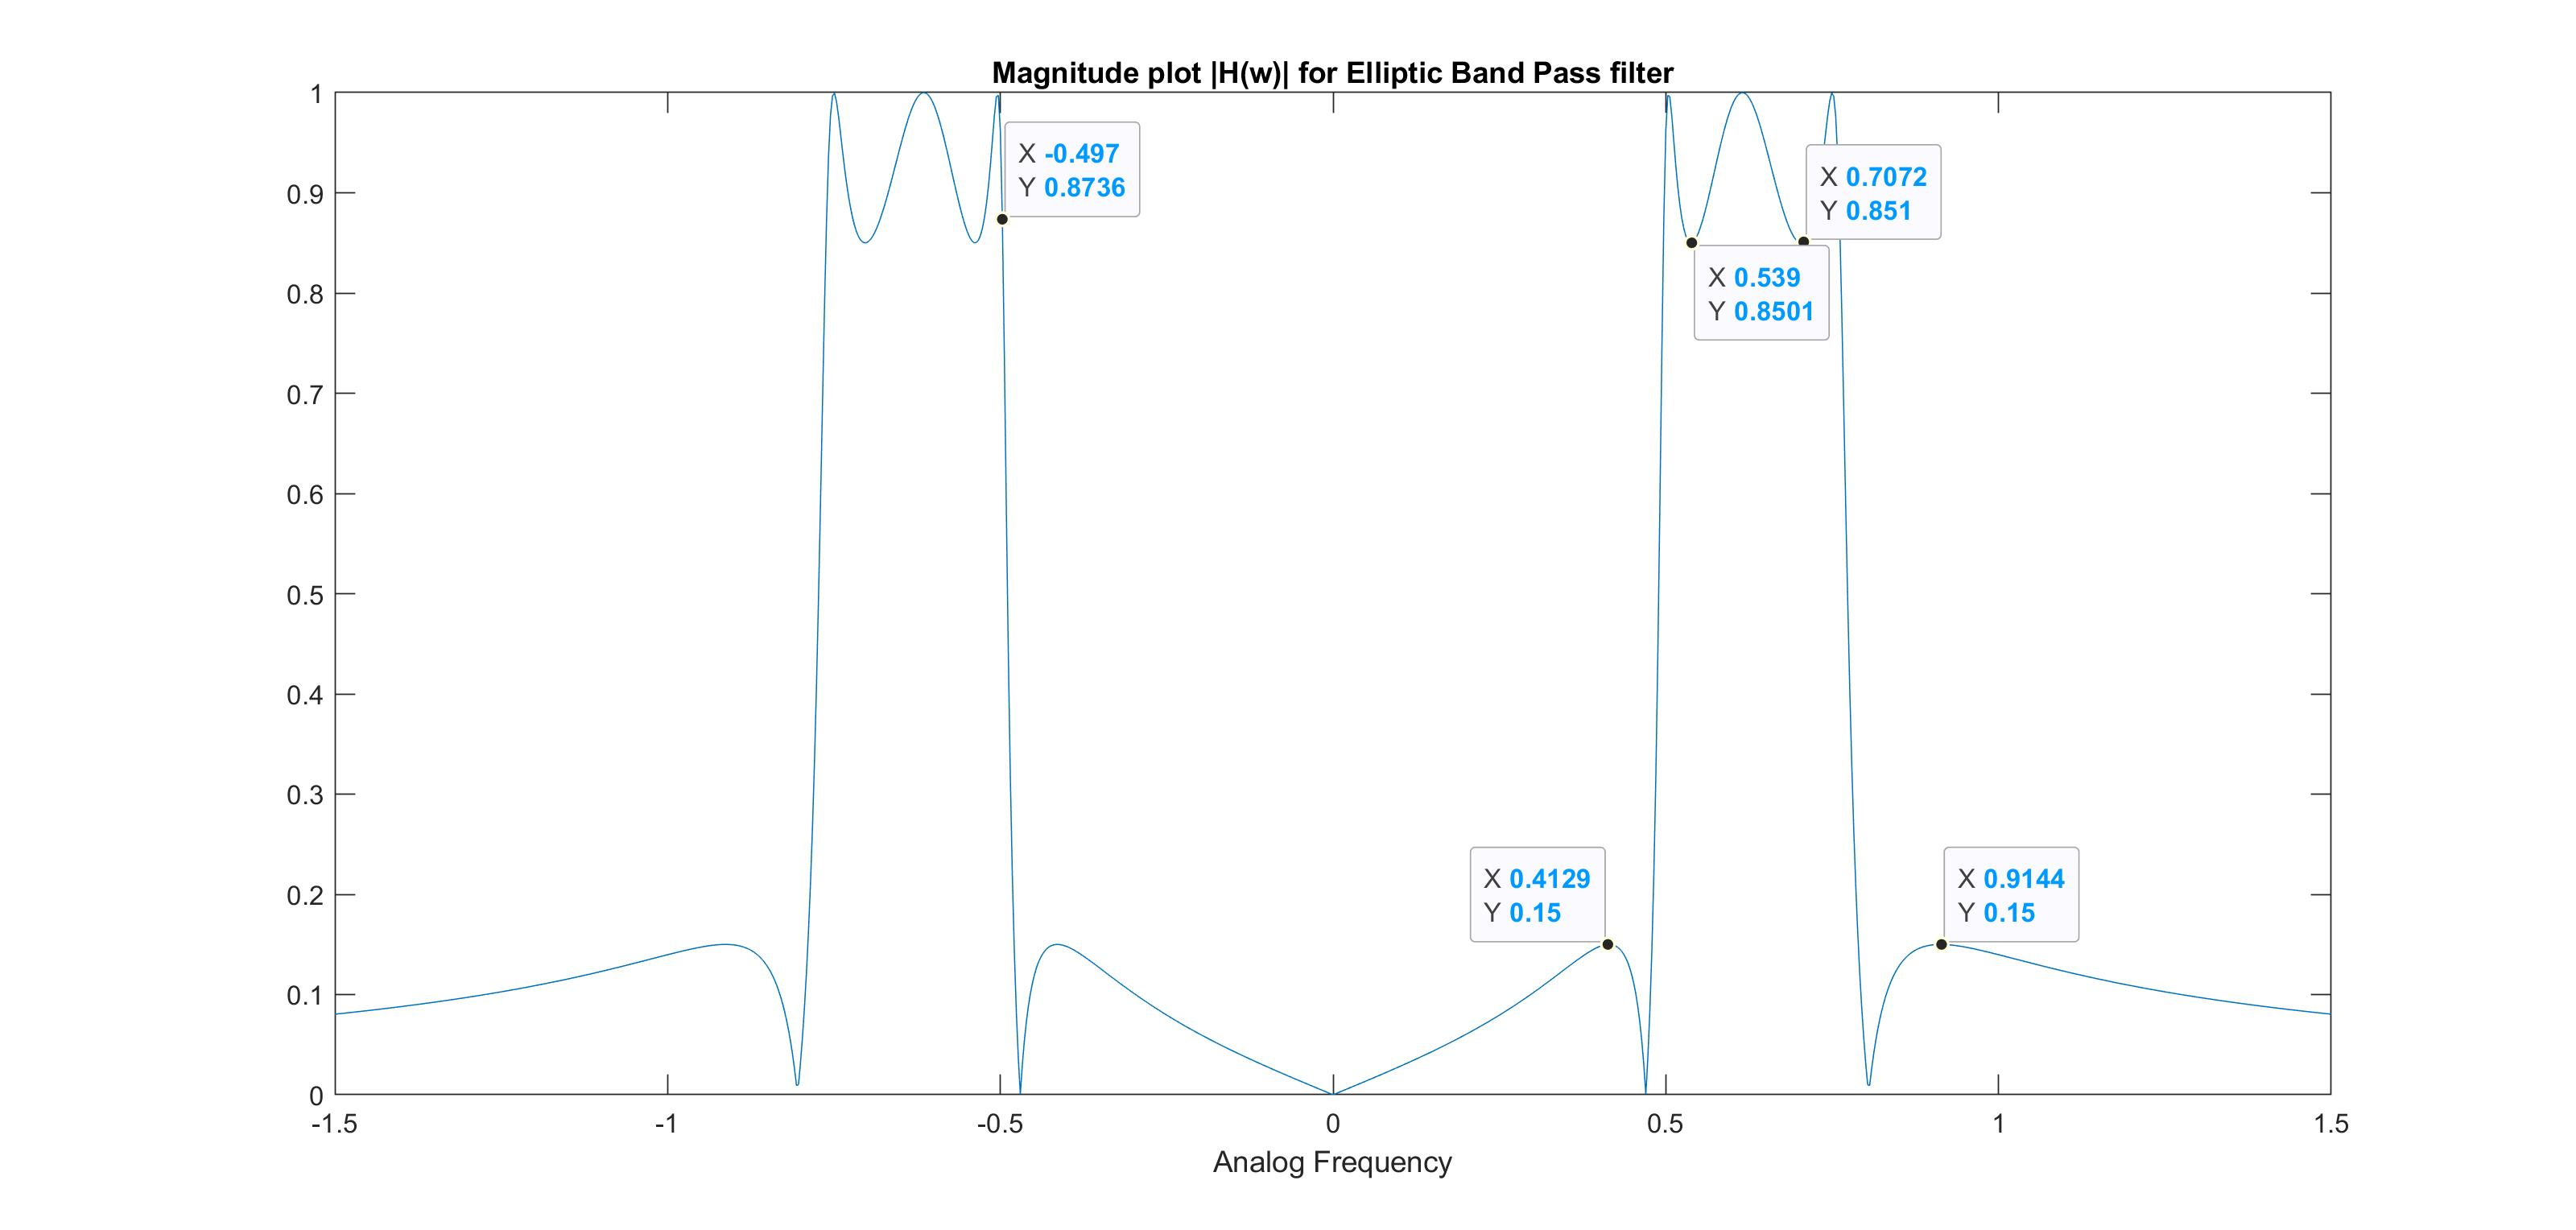
\includegraphics[width = 18cm, trim=1cm 0cm 1cm 0cm, clip]{Filter3ABPF.jpg}
\end{figure}


\color{cyan}
\subsection{Discrete time Band Pass Transfer function}
\color{black}
Using the Bilinear Transformation:
\begin{gather*}
	s = \frac{1-z^{-1}}{1+z^{-1}}
\end{gather*}
Substituting this back into $H_{Analog,BPF}(s)$, we get $H_{digital,BPF}$ as
\begin{gather*}
	\frac{0.0661 - 0.1127z^{-1} + 0.1022z^{-2} - 0.1022z^{-4} + 0.1127z^{-5} - 0.0661z^{-6} }{1 - 2.5107z^{-1} +4.6918z^{-2} - 5.0106z^{-3} + 4.2212z^{-4} - 2.0205z^{-5} + 0.721z^{-6}}
\end{gather*}

\begin{figure}[H]
	\centering
	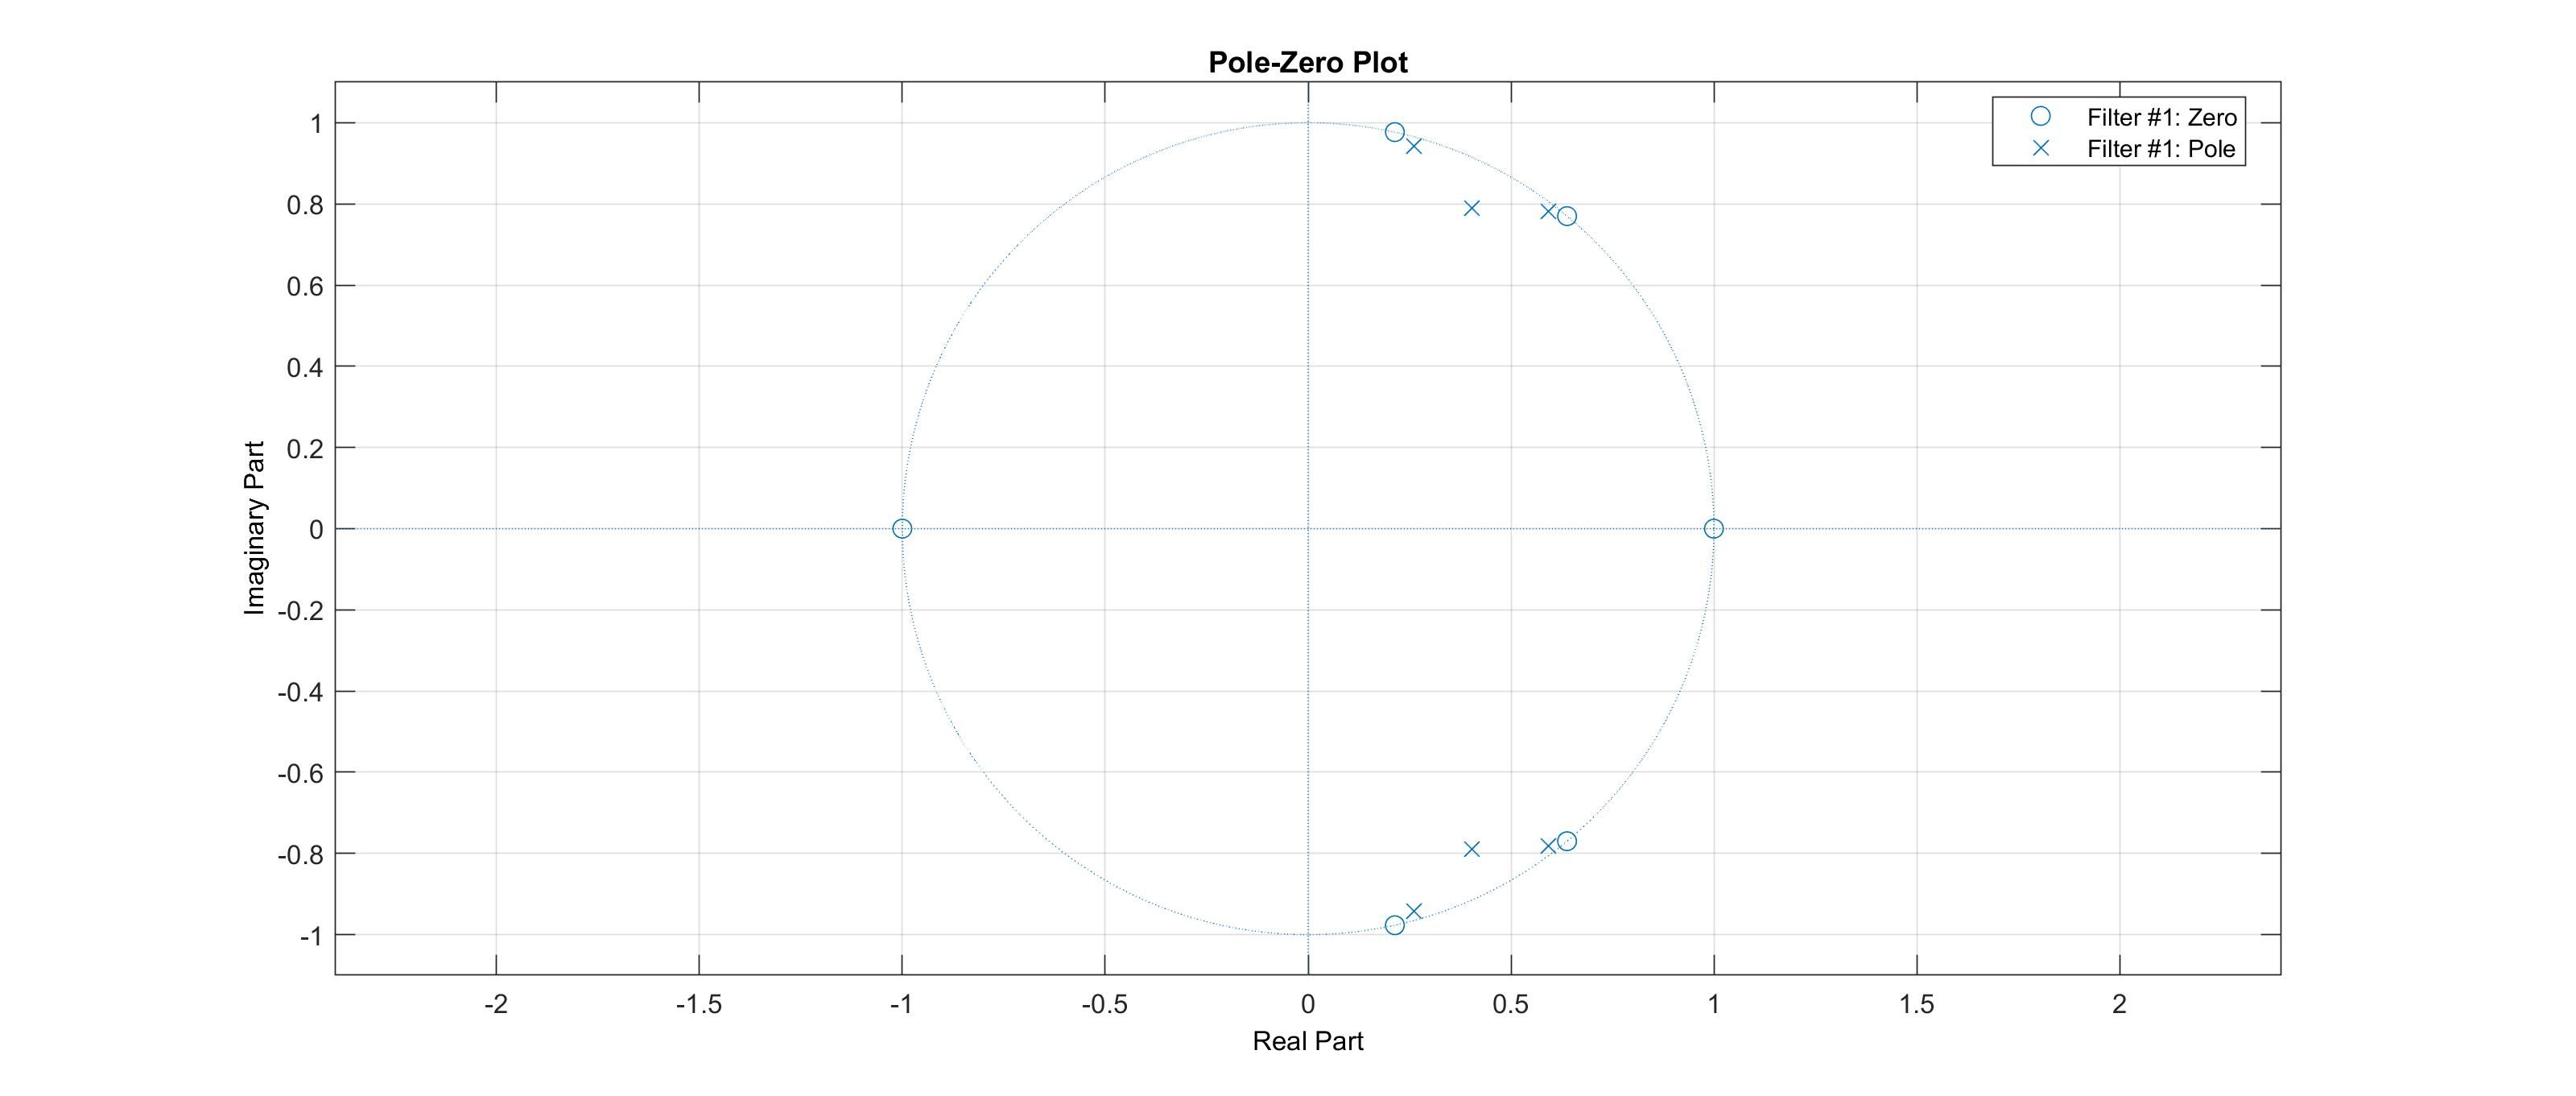
\includegraphics[width = 18cm]{Filter3PZ.jpg}
\end{figure}

\begin{figure}[H]
	\centering
	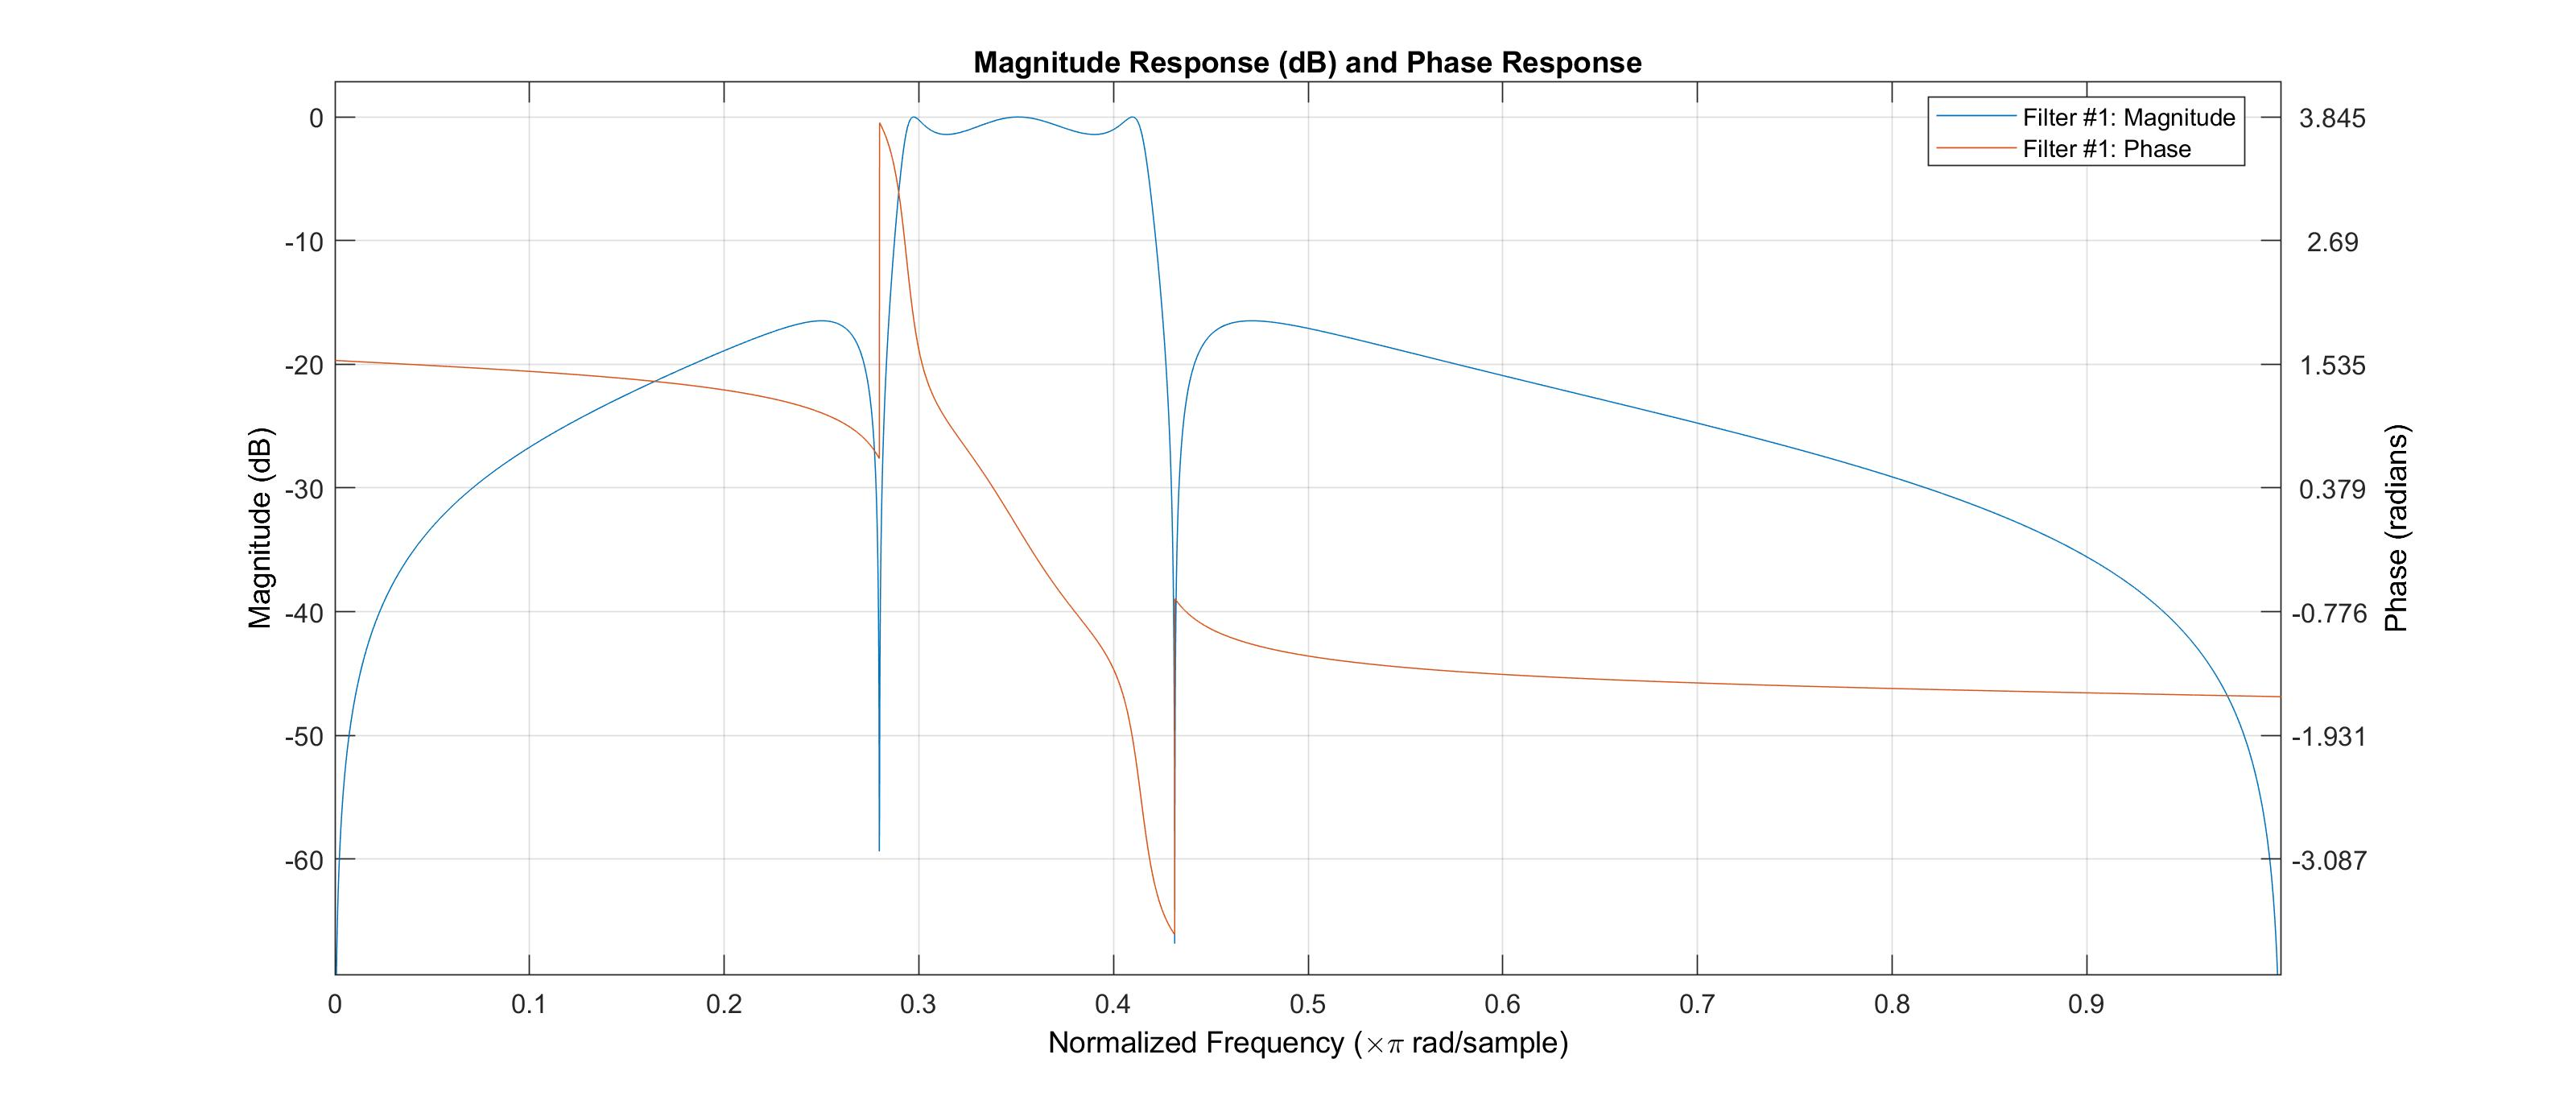
\includegraphics[width = 18cm, height = 10cm]{Filter3MagPhase.jpg}
\end{figure}
\begin{figure}[H]
	\centering
	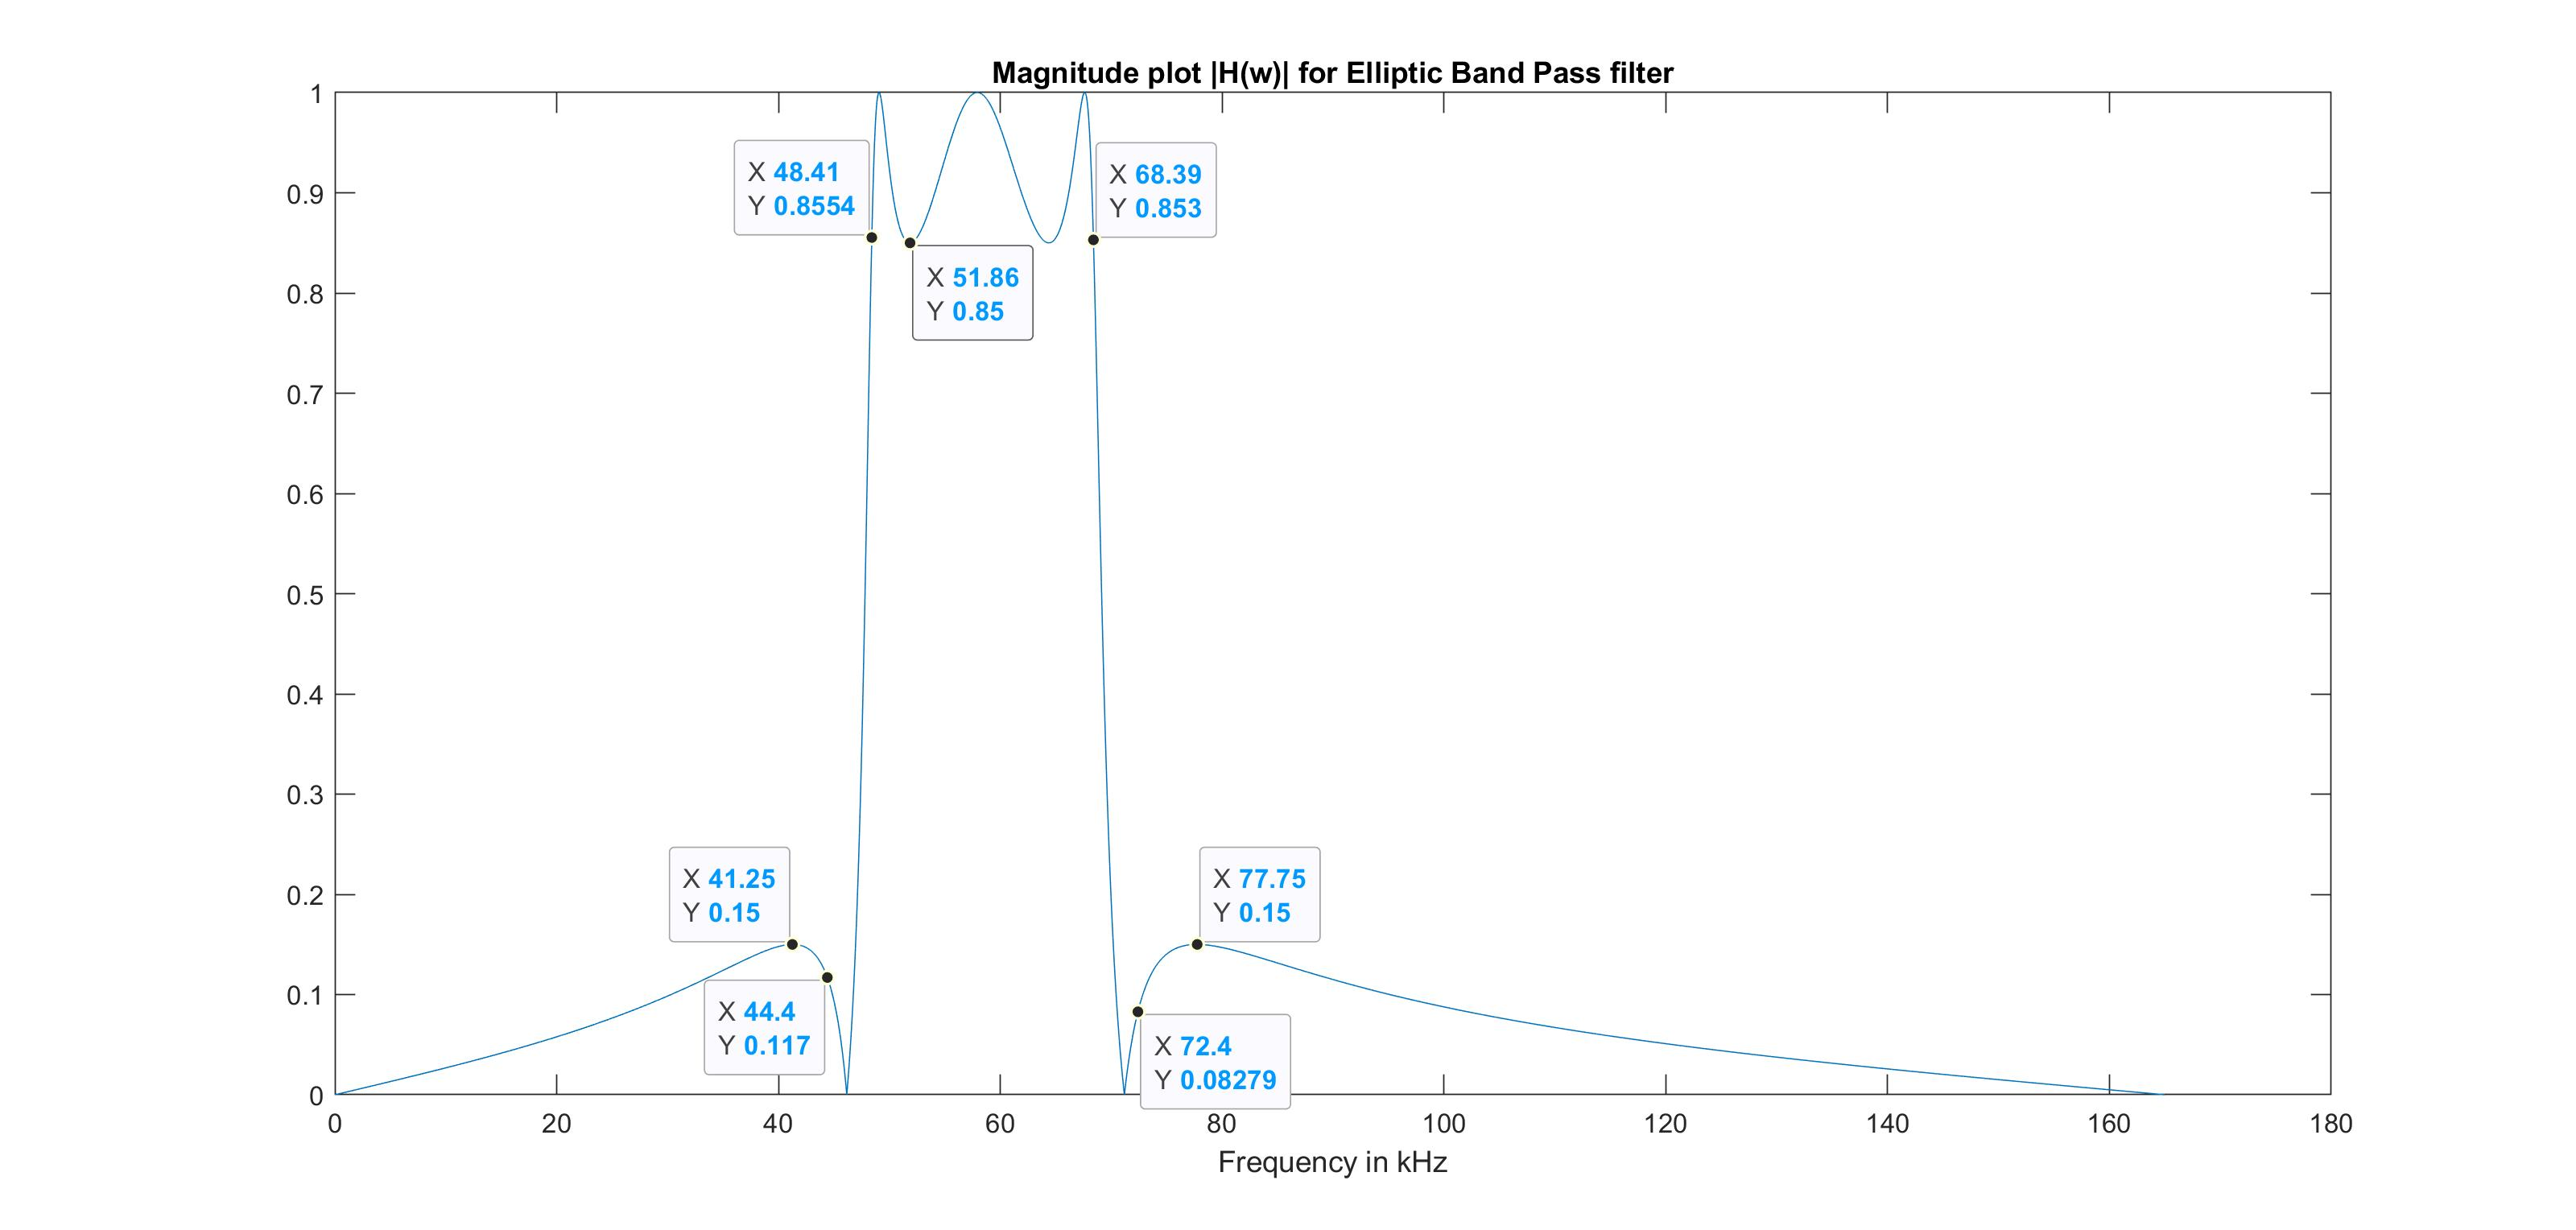
\includegraphics[width = 18cm, trim=0cm 0cm 0cm 0cm, clip]{Filter3DBPF.jpg}
\end{figure}

\color{cyan}
\subsection{Review report}
\color{black}
\newpage

\color{darkblue}
\section{Filter 2: Elliptic Band Stop Filter}
\color{black}
\begin{itemize}
	\item Filter Number Assigned = m = 33
	\item Both Pass band and Stop band tolerances are 0.15
	\item Pass Band is Equiripple 
	\item Stop band is Equiripple 
	\item Elliptic / Jacobi Approximation
	\item Band-stop Filter
	\item The Transition band is 4kHz on either side of the stop band
	\item The input signal is Band limitted to 120kHz and the sampling rate is 260kHz.
\end{itemize}
\color{cyan}
\subsection{Unnormalized Specifications}
\color{black}
m = 33\\
q(m) = 3\\
r(m) = 33 - 30 = 3\\
BL(m) = 25 + 1.9 $\times$ 3 + 4.1 $\times$ 3 = 43 kHz\\
BH(m) = BL(m) + 20 = 63 kHz\\

\noindent Hence the filter specifications for the Band-stop Filter are:
\begin{itemize}
	\item Stop band is 43 kHz to 63 kHz
	\item Transition band is 4kHz on either side of the Stop band
	\item Pass band is 0 to 39 kHz and 67 kHz to 130 kHz
	\item Tolerances for both bands are 0.15
	\item Both Stop band and Pass band are Equiripple

\end{itemize}

\color{cyan}
\subsection{Normalized specifications}
\color{black}
Given sampling rate  = 260 kHz. Using\\
\begin{gather*}
	\omega = \frac{2\pi \ast \Omega}{\Omega_s}
\end{gather*}
where $\omega$ is the normalized frequency, $\Omega$ is the Un-normalized frequency and $\Omega_s$ is the sampling frequency.
\begin{itemize}
	\item Stop band is $\frac{43}{130}\pi$ to $\frac{63}{130}\pi$ $\sim$ (0.33$\pi$ to 0.48$\pi$)
	\item Transition band is $\frac{4}{130}\pi$ $\sim$ (0.03$\pi$) on either side of the Stop band
	\item Pass band is 0 to  $\frac{3}{10}\pi$ and $\frac{67}{130}\pi$ to $\pi$  $\sim$ (0 to 0.3$\pi$ and  0.52$\pi$ to $\pi$)
	\item Tolerances for both bands are 0.15
	\item Both Stop band and Pass band are Equiripple
\end{itemize}

\color{cyan}
\subsection{Analog Band-stop Filter Specifications}
\color{black}
Using Bilinear Transformation,
\begin{gather*}
	\Omega = tan\left(\frac{\omega}{2}\right)
\end{gather*}
where $\Omega$ is the analog domain frequency and $\omega$ is the discrete domain frequency\\

\begin{center}
	\begin{tabular}{ |c|c|c|c|c|c|c| }
		\hline
		&&&&&&\\
		Domain & Zero & $\Omega_{P1}$ & $\Omega_{S1}$ &$\Omega_{S2}$& $\Omega_{P2}$& Infinity\\
		&&&&&&\\
		\hline
		&&&&&&\\
		$\omega$ & 0 & $\frac{3}{10}\pi$ & $\frac{43}{130}\pi$& $\frac{63}{130}\pi$& $\frac{67}{130}\pi$& $\pi$\\
		&&&&&&\\
		\hline
		&&&&&&\\
		$\Omega$ & 0 & 0.5095 & 0.572 & 0.9528 & 1.0495 & $\infty$\\
		&&&&&&\\
		\hline
	\end{tabular}
\end{center}

\noindent Hence the filter specifications for the corresponding analog domain Bandstop Filter are:
\begin{itemize}
	\item Stop band is 0.572 ($\Omega_{S1}$)  to 0.9528 ($\Omega_{S2}$) 
	\item Pass band is 0 to 0.5095($\Omega_{P1}$) and 1.0495 ($\Omega_{P2}$) to $\infty$
	\item Tolerances for both bands are 0.15
	\item Both Stop band and Pass band are Equiripple
\end{itemize}

\color{cyan}
\subsection{Frequency Transformation in to a Low Pass Filter}
\color{black}
Using the Band-Stop Transformation
\begin{gather*}
	\Omega_L = \frac{B\Omega}{\Omega_0^2 - \Omega^2}\\\\
	\Omega_0 = \sqrt{\Omega_{P1} \Omega_{P2}} = 0.7313\\\\
	B = \Omega_{P2} - \Omega_{P1} = 0.54
\end{gather*}

\begin{center}
	\begin{tabular}{ |c|c|c|c|c|c|c|c|c| }
		\hline
		&&&&&&&&\\
		Domain & Zero & $\Omega_{P1}$ & $\Omega_{S1}$ &$\Omega_0^-$ &$\Omega_0^+$ & $\Omega_{S2}$& $\Omega_{P2}$ & Infinity\\
		&&&&&&&&\\
		\hline
		&&&&&&&&\\
		$\Omega$ & 0$^+$ & 0.5095 & 0.572 &0.7313 &0.7313&0.9528& 1.0495 & +$\infty$\\
		&&&&&&&&\\
		\hline
		&&&&&&&&\\
		$\Omega_L$ & 0$^+$ & 1 & 1.4879 & +$\infty$ & -$\infty$ & -1.3792 & -1 & 0$^-$\\
		&&&&&&&&\\
		\hline
		&&&&&&&&\\
		Domain& Zero & $\Omega_{LP1}$ & $\Omega_{LS1}$ &+Infinity &-Infinity & $\Omega_{LS2}$& $\Omega_{LP2}$ &Zero\\
		&&&&&&&&\\
		\hline
	\end{tabular}
\end{center}

\color{cyan}
\subsection{Analog Low Pass Filter Specification}
\color{black}
Hence the Frequency Transformed Low-Pass Filter Specifications are:
\begin{itemize}
	\item Pass band edge is at 1 ($\Omega_{LP}$)
	\item Stop band edge = min (-$\Omega_{LS2}$, $\Omega_{LS1}$) = 1.3792 ($\Omega_{LS}$)
	\item Tolerances = 0.15 for both Stop band and Pass band
	\item Both Stop band and Pass band are Equiripple
\end{itemize}


\color{cyan}
\subsection{Analog Low Pass Filter Transfer function}
\color{black}
The magnitude-squared frequency response of an elliptic filter is defined as
\begin{gather*}
	H_{analog,LPF}^2(j\Omega) = \frac{1}{1+\epsilon^2R_{n}^2(\Omega, \Omega_{LS}, \delta_1, \delta_2)}
\end{gather*}
Where $R_n$ is the nth-order elliptic rational function also known as a Chebyshev rational function. The order n, $\epsilon$ and will depend on the required specifications.
The minimum order required can be calculated using the following steps,
\begin{gather*}
	\delta_1 = \delta_2 = 0.15\\
	D_1 = \frac{1}{(1-\delta_1)^2} - 1 = 0.3841\\
	D_2 = \frac{1}{\delta_2^2} - 1 = 43.4444\\
	\epsilon = \sqrt{D1} = 0.61975\\
	k = \frac{\Omega_{LP}}{\Omega_{LS}} =  \frac{1}{1.3792} = 0.72505\\
	k' = \sqrt{1-k^2} = 0.6886\\
	k_1 = \sqrt{\frac{D1}{D2}} = 0.094\\
	k_1' = \sqrt{1-k_1^2} = 0.99557\\
	Nmin \ge \frac{KK_1'}{K'K_1}
\end{gather*}
Where K, K', $K_1$, $K_1'$ are the values of complete elliptic integrals evaluated at k, k', $k_1$, $k_1'$.\\
We get, K = 1.8765 , K' = 1.8329, $K_1$ = 1.5743, $K_1'$ = 3.7566. Using these values, we get the order of the elliptic rational function as 3. Once we get $N_{min}$, we need to recompute k and $\Omega_{LS}$ for all the conditions to be satisfied.
\begin{gather*}
	Nmin = \ceil{2.443} = 3 
\end{gather*}
Where, Elliptic integral is defined as,
\begin{gather*}
	u(\phi,k) = \int_{0}^{\phi} \frac{dy}{\sqrt{1-k^2sin^2(y)}}
\end{gather*} 
and complete elliptic integral is equal to u($\pi$/2, k). i.e,
\begin{gather*}
	U(k) = \int_{0}^{\pi/2} \frac{dy}{\sqrt{1-k^2sin^2(y)}}
\end{gather*}
Using the above elliptic integral equation we can also write $\phi$ in terms of $u$,k. i.e, $\phi(u$,k). This is the inverse of elliptic integral function. Using this we can define Jacobi elliptic sine function and other elliptic functions are defined as,
\begin{gather*}
	sn(u,k) = sin(\phi(u,k))\\
	cn(u,k) = cos(\phi(u,k))\\
	dn(u,k) = \sqrt{1-k^2sn^2(u,k)}\\
	cd(u,k) = \frac{cn(u,k)}{dn(u,k)}
\end{gather*}
The Chebyshev rational function can be represented as,
\begin{gather*}
	R_n(\Omega) = sn(N_{min}\times sn^{-1}(\Omega,k),k_1)\\
	R_n(\Omega) = sn(\phi,k_1), \Omega = sn(\phi,k)
\end{gather*}
The zero locations of the Transfer function can be given by,
\begin{gather*}
	\Omega = \frac{\pm1}{k cd(iK/N_{min},k)}, i.e.,\\
	s = \frac{\pm j}{k cd(iK/N_{min},k)}
\end{gather*}
Where i = 0, 2, 4, ..., N-1 for Odd N, and i = 1, 3, 5, ... N-1 for Even N.\\
The pole locations of the transfer function can be given by,
\begin{gather*}
	1 + \epsilon^2R_n(s/j)^2 = 0
\end{gather*}
Using the periodicity of sn(u,k), we get
\begin{gather*}
	sn(N_{min}\phi, + 2K_1i,k_1) = \pm j\frac{1}{\epsilon}\\
	\phi = (-2Ki + sn^{-1}(\frac{j}{\epsilon},k_1))/N_{min}\\
	\Omega = sn(\phi,k)
\end{gather*}

\noindent Define, 
\begin{gather*}
	jV_0 = sn^{-1}(\frac{j}{\epsilon},k_1)/N_{min}
\end{gather*}

Using these equations, location of poles can be found using
\begin{gather*}
	s = j sn(Ki/N + jV_0,k) = jcd(Ki/N + (1-jV_0),k)
\end{gather*}
Note that here j represents complex number and i = 0, 2, 4, ..., N-1 for Odd N, and i = 1, 3, 5, ... N-1 for Even N.
From the above equations, the poles and zeroes are found to be:
\begin{verbatim}
	
	p1=-0.11533-0.9936i
	p2=-0.11533+0.9936i
	p3=-0.6232
	z1=-1.2604i
	z2=1.2604i 
\end{verbatim}
Using these poles and zeroes the transfer function Low pass analog filter is given by,

\begin{gather*}
	H_{analog,LPF}(s_{L}) = \frac{0.3925s_L^2 + 0.6235}{s_L^3 + 0.8538s_L^2 + 1.1443s_L + 0.6235}	
\end{gather*}

\begin{figure}[H]
	\centering
	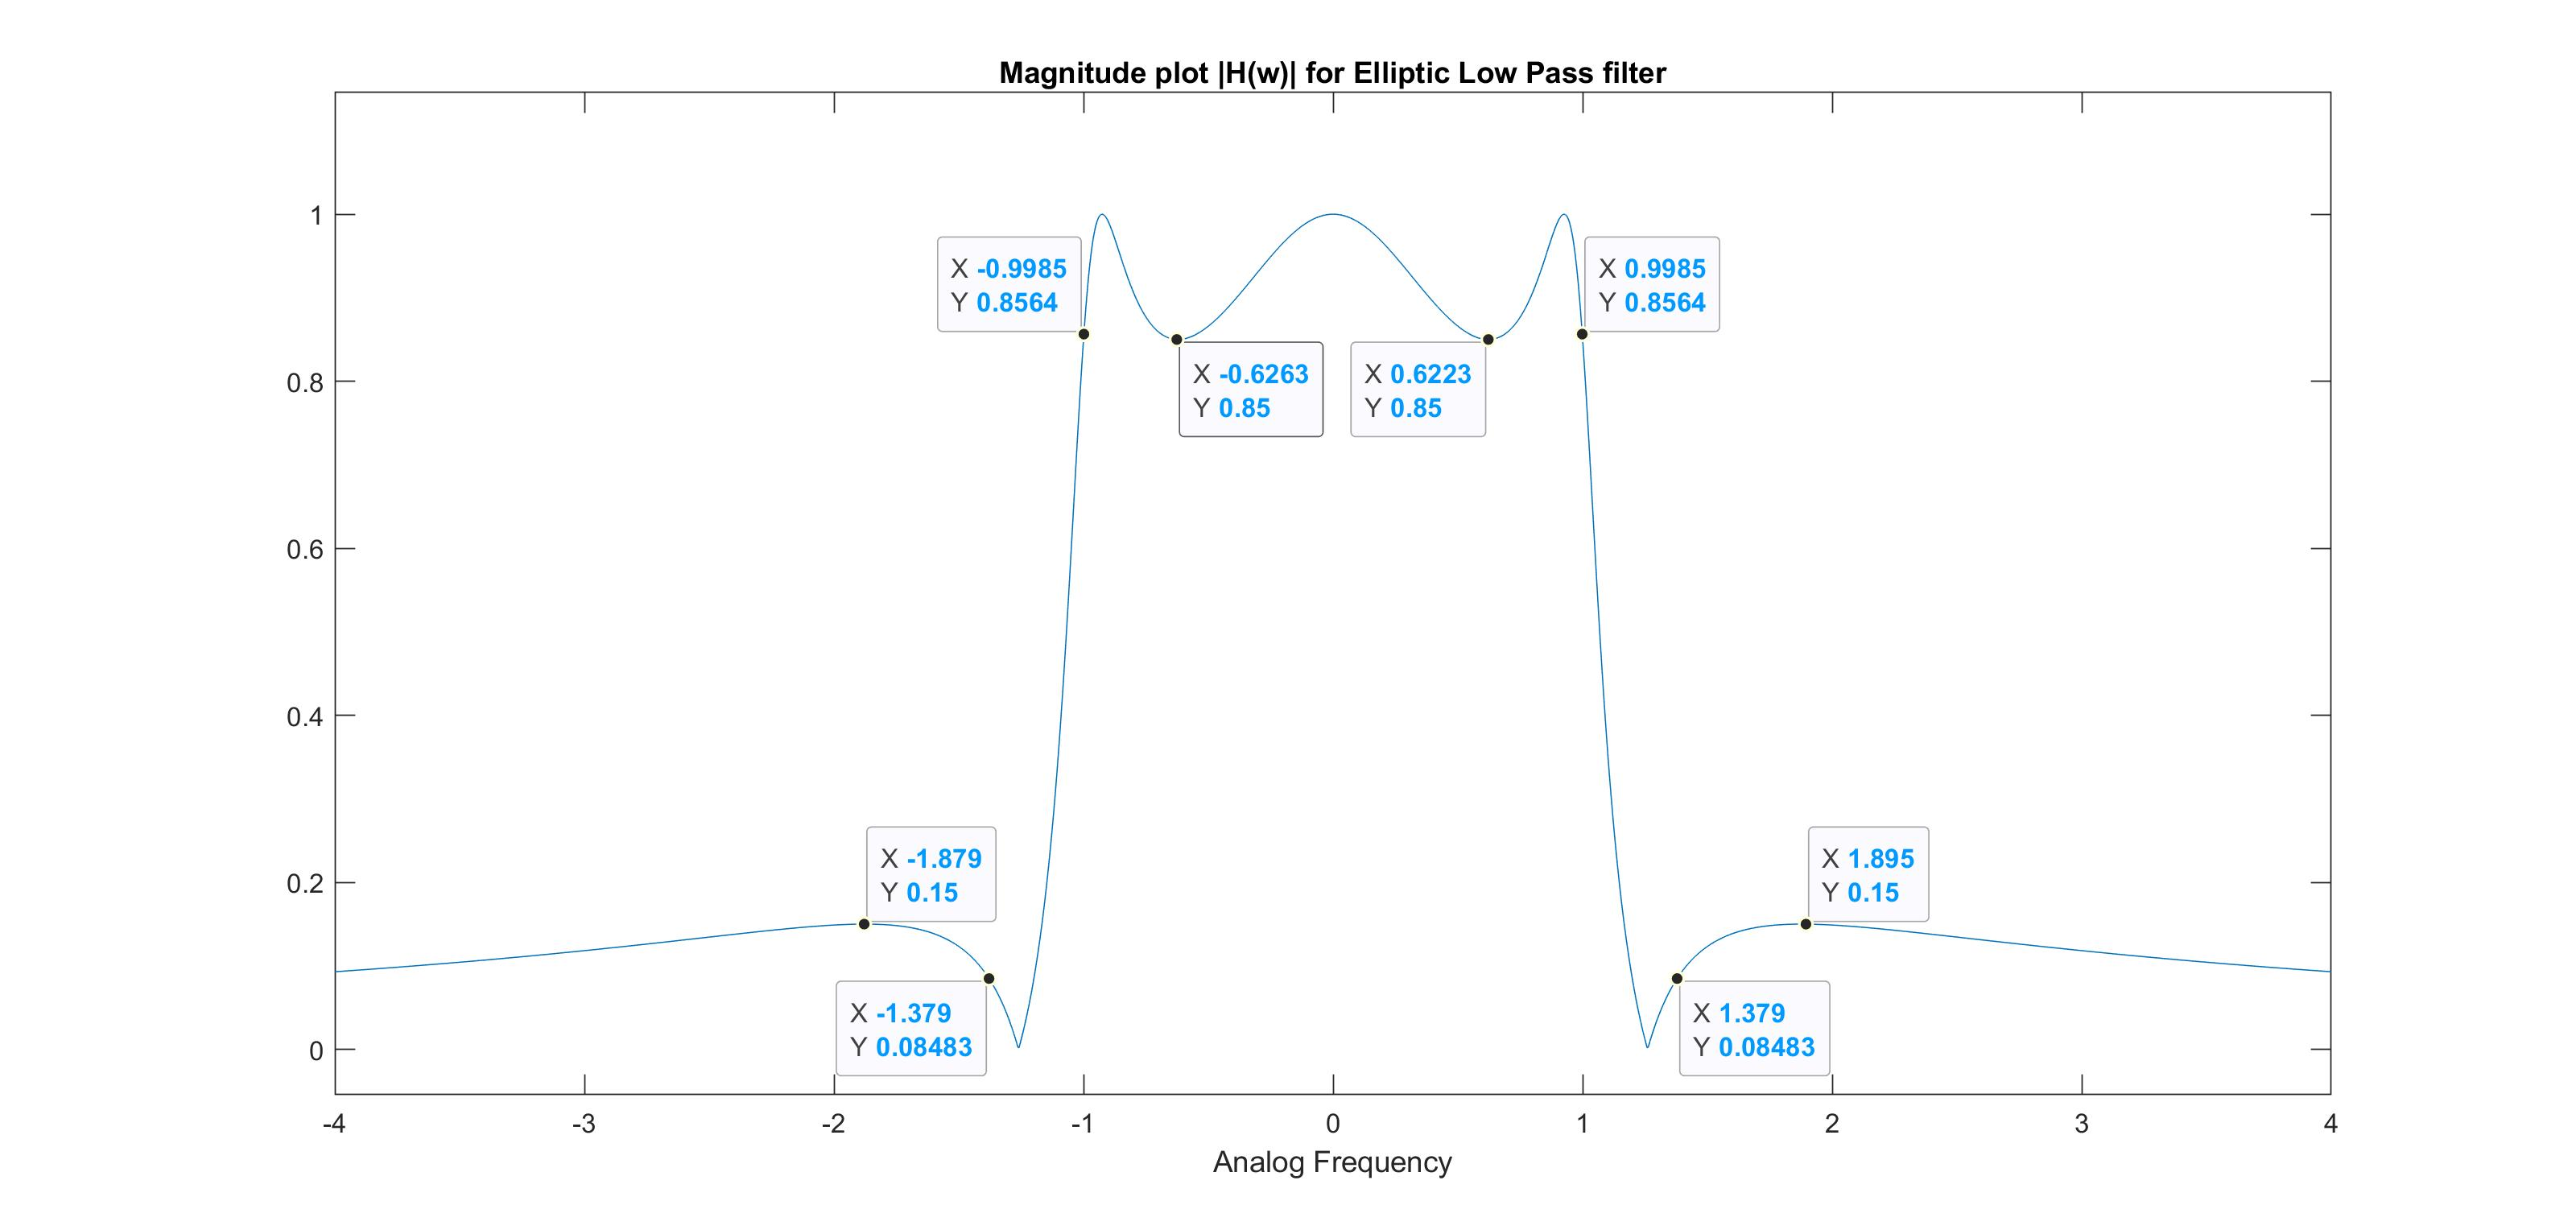
\includegraphics[width = 18cm]{Filter4ALPF.jpg}
\end{figure}

\color{cyan}
\subsection{Analog Band Stop Transfer function}
\color{black}
Using the Band Stop Transformation:
\begin{gather*}
	s_L = \frac{Bs}{s^2 + \Omega_0^2}
\end{gather*}
Substituting the values B = 0.54 and $\Omega_0$ = 0.7313,
\begin{gather*}
	s_L = \frac{0.54s}{s^2 + 0.535}
\end{gather*}

\noindent Substituting this back into $H_{analog,LPF}$, we get $H_{analog,BSF}$ as
\begin{gather*}
	\frac{s^6 + 1.7879s^4 +0.9561s^2 + 0.1529}{s^6 + 0.9911s^5 + 2.0036s^4 + 1.3126s^3 + 1.0715s^2 + 0.2834s + 0.1529}	
\end{gather*}
\begin{figure}[H]
	\centering
	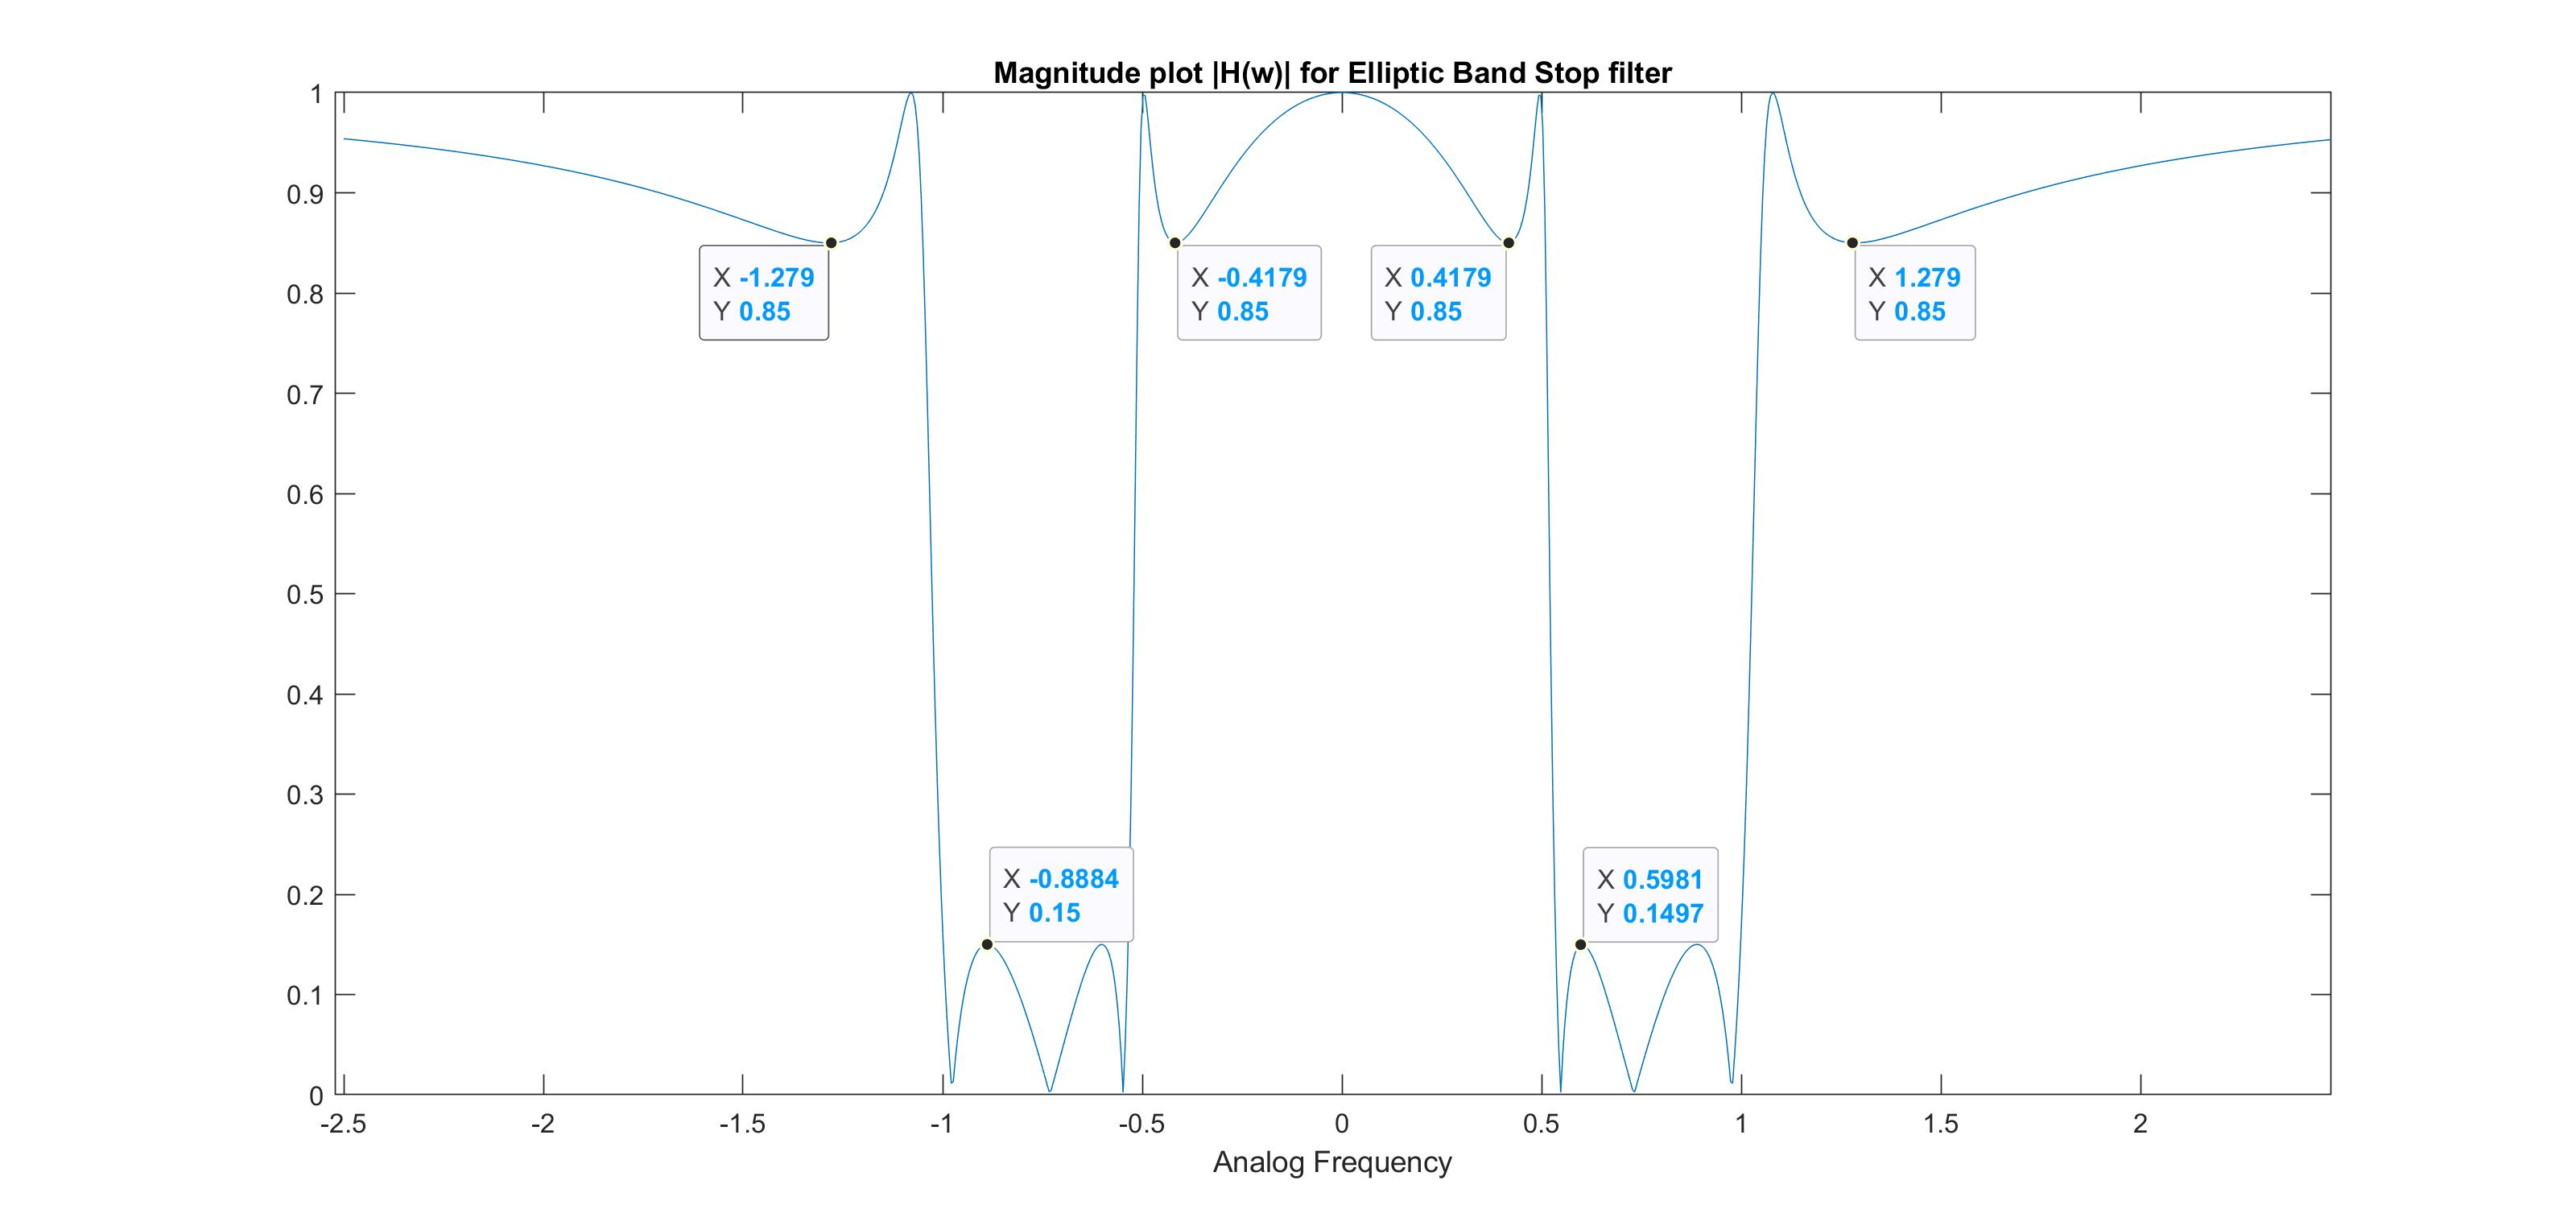
\includegraphics[width = 16cm, trim=1cm 0cm 1cm 0cm, clip]{Filter4ABSF.jpg}
\end{figure}

\color{cyan}
\subsection{Discrete time Band Stop Transfer function}
\color{black}
Using the Bilinear Transformation:
\begin{gather*}
	s = \frac{1-z^{-1}}{1+z^{-1}}
\end{gather*}
Substituting this back into $H_{Analog,BPF}(s)$, we get $H_{digital,BSF}$ as
\begin{gather*}
	\frac{0.5718 - 0.9899z^{-1} + 0.2135z^{-2} - 1.9977z^{-3} + 2.1350z^{-4} - 0.9899z^{-5} + 0.5718z^{-6}}{1 - 1.4347z^{-1} + 2.4436z^{-2} - 1.9388z^{-3} + 1.7291z^{-4} - 0.604z^{-5} + 0.2408z^{-6}}
\end{gather*}
\begin{figure}[H]
	\centering
	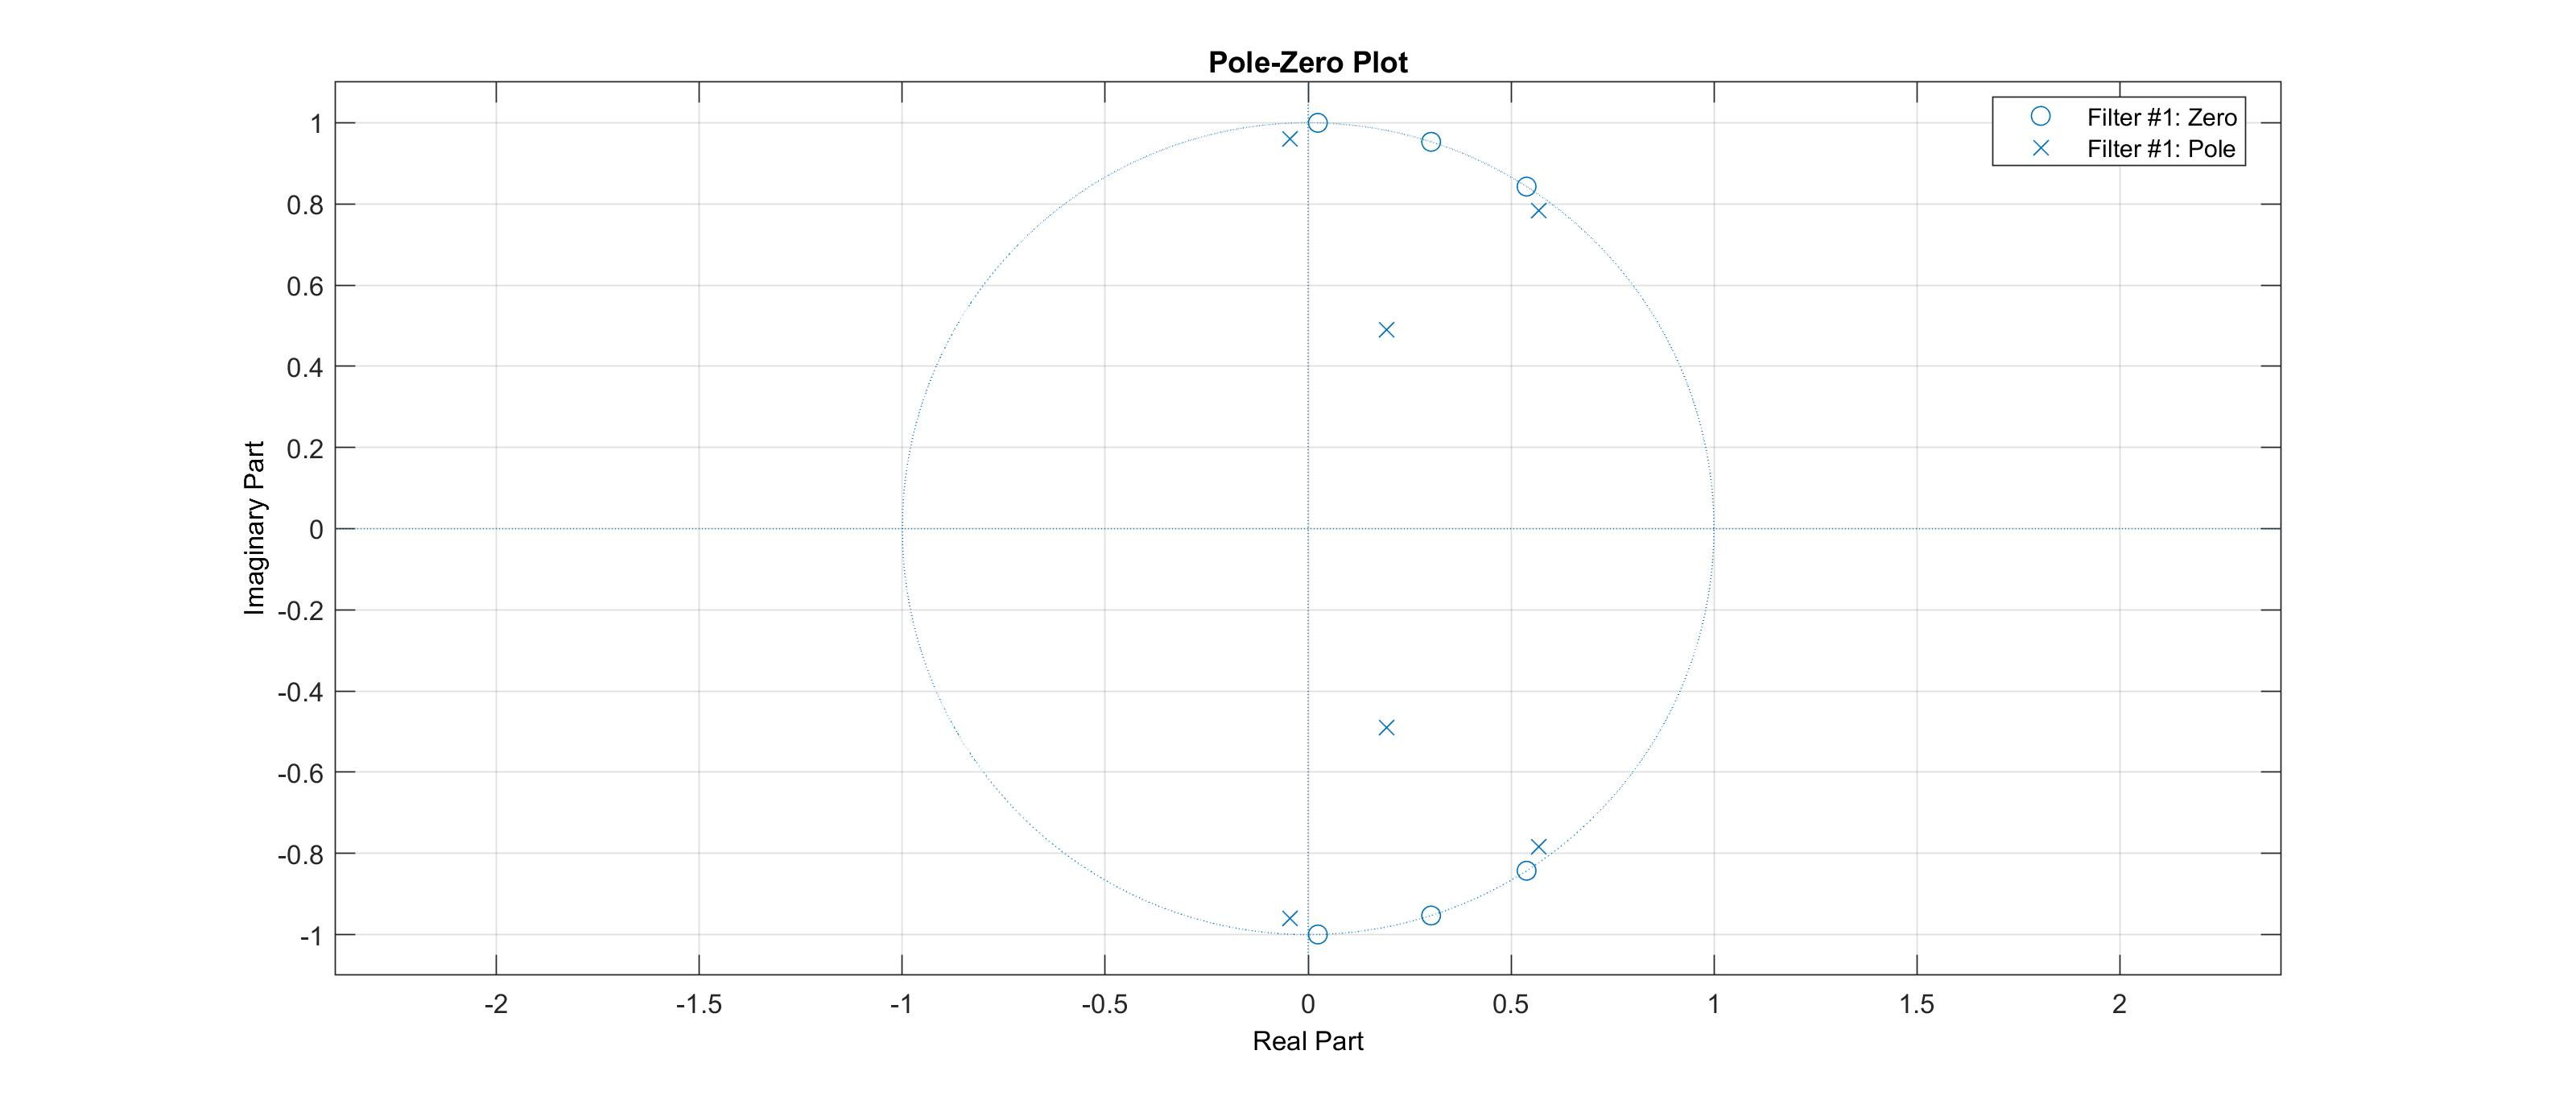
\includegraphics[width = 18cm]{Filter4PZ.jpg}
\end{figure}
\begin{figure}[H]
	\centering
	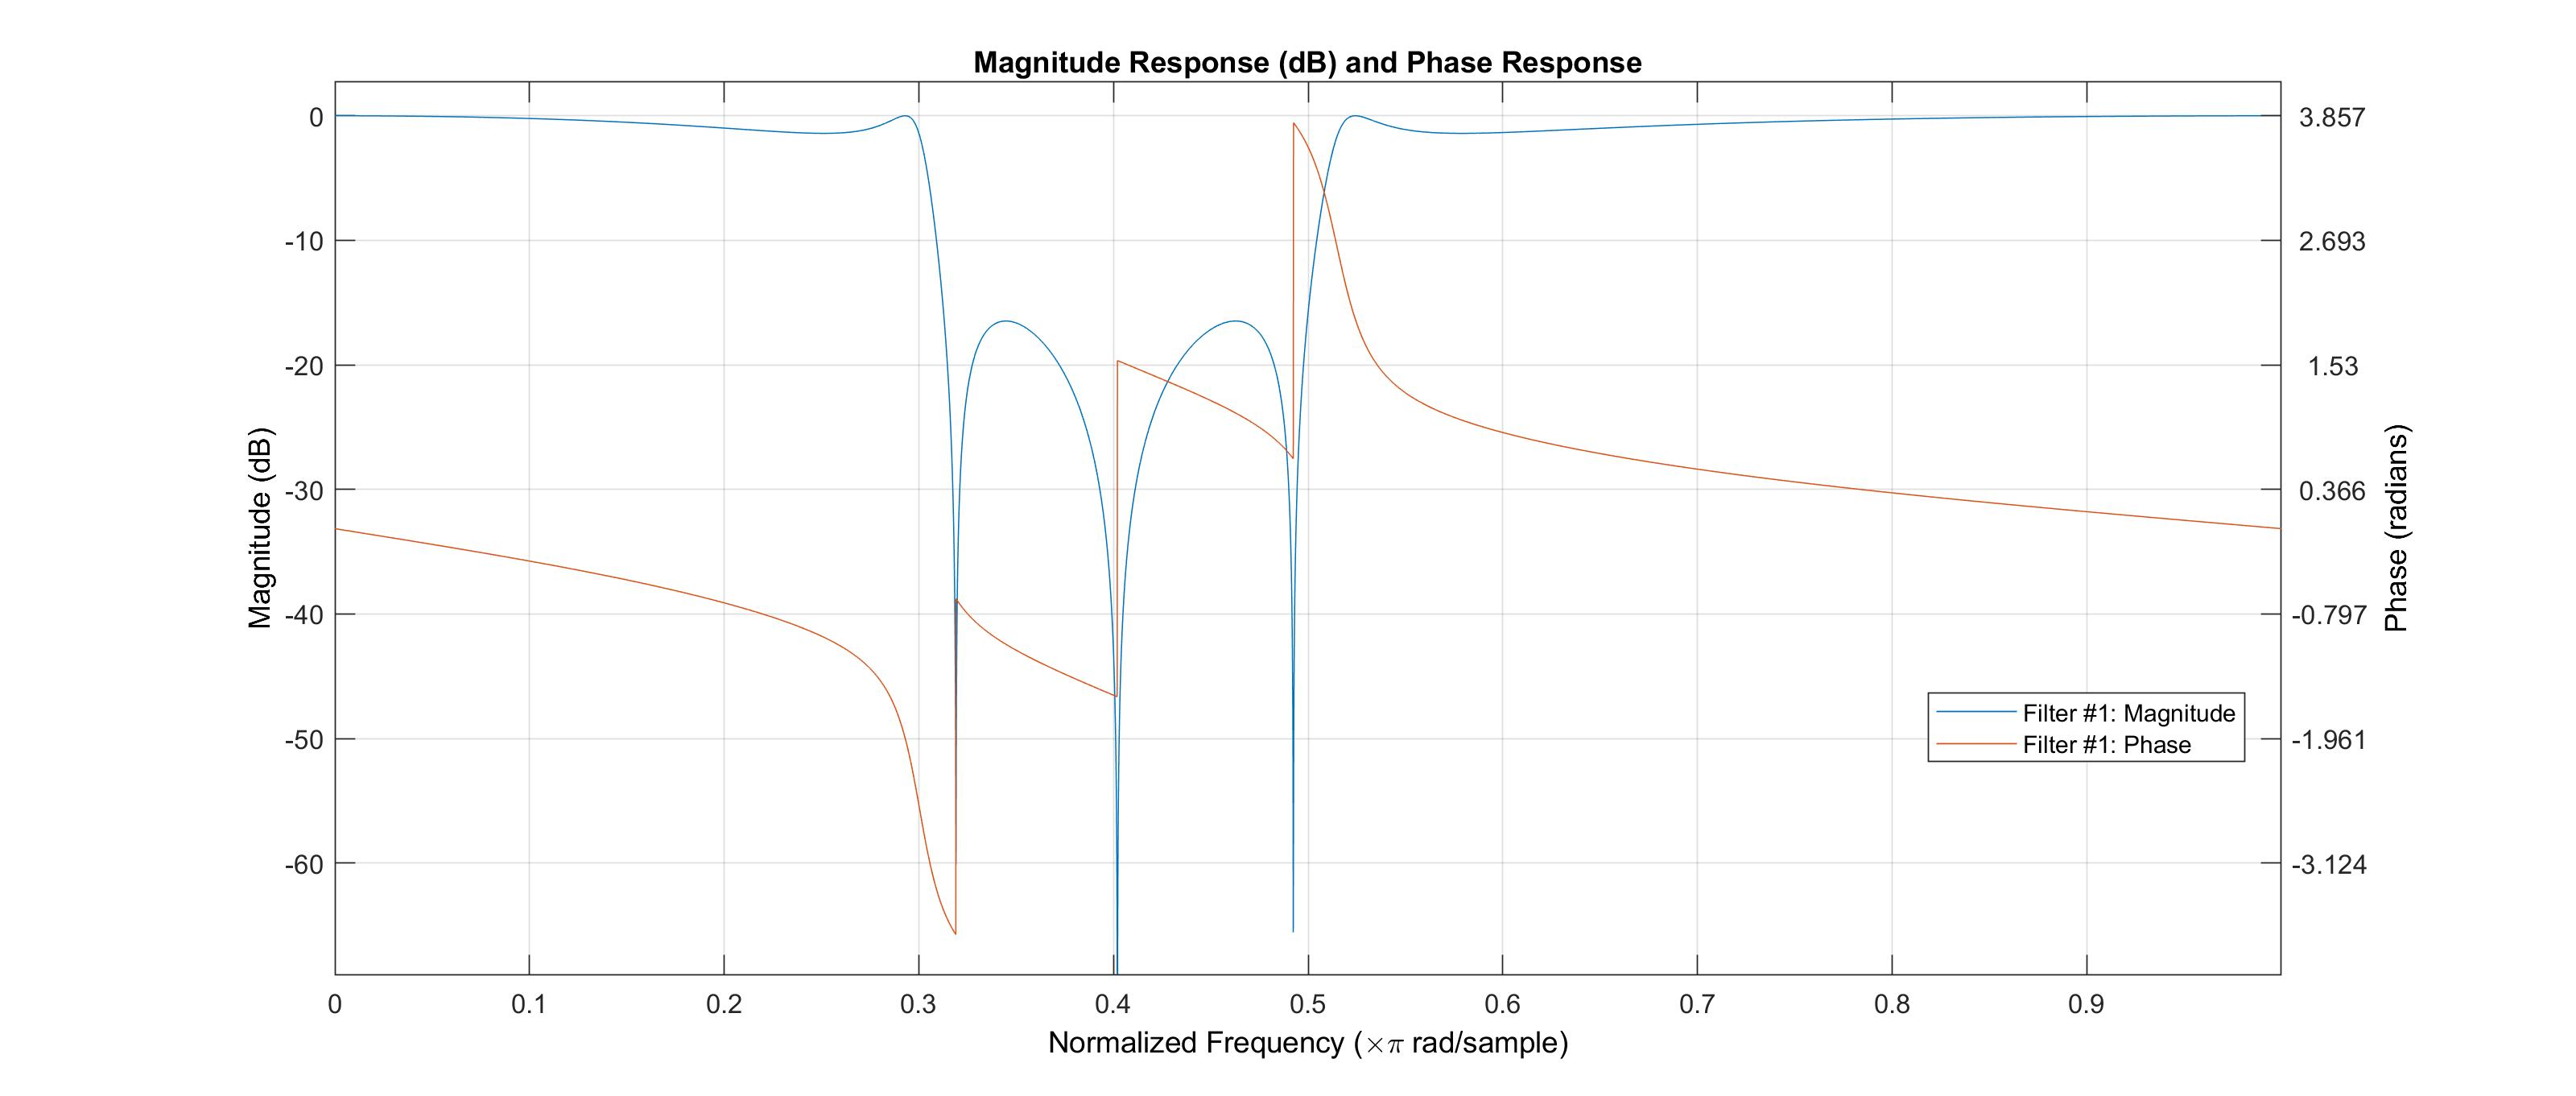
\includegraphics[width = 18cm, height = 10cm]{Filter4MagPhase.jpg}
\end{figure}
\begin{figure}[H]
	\centering
\	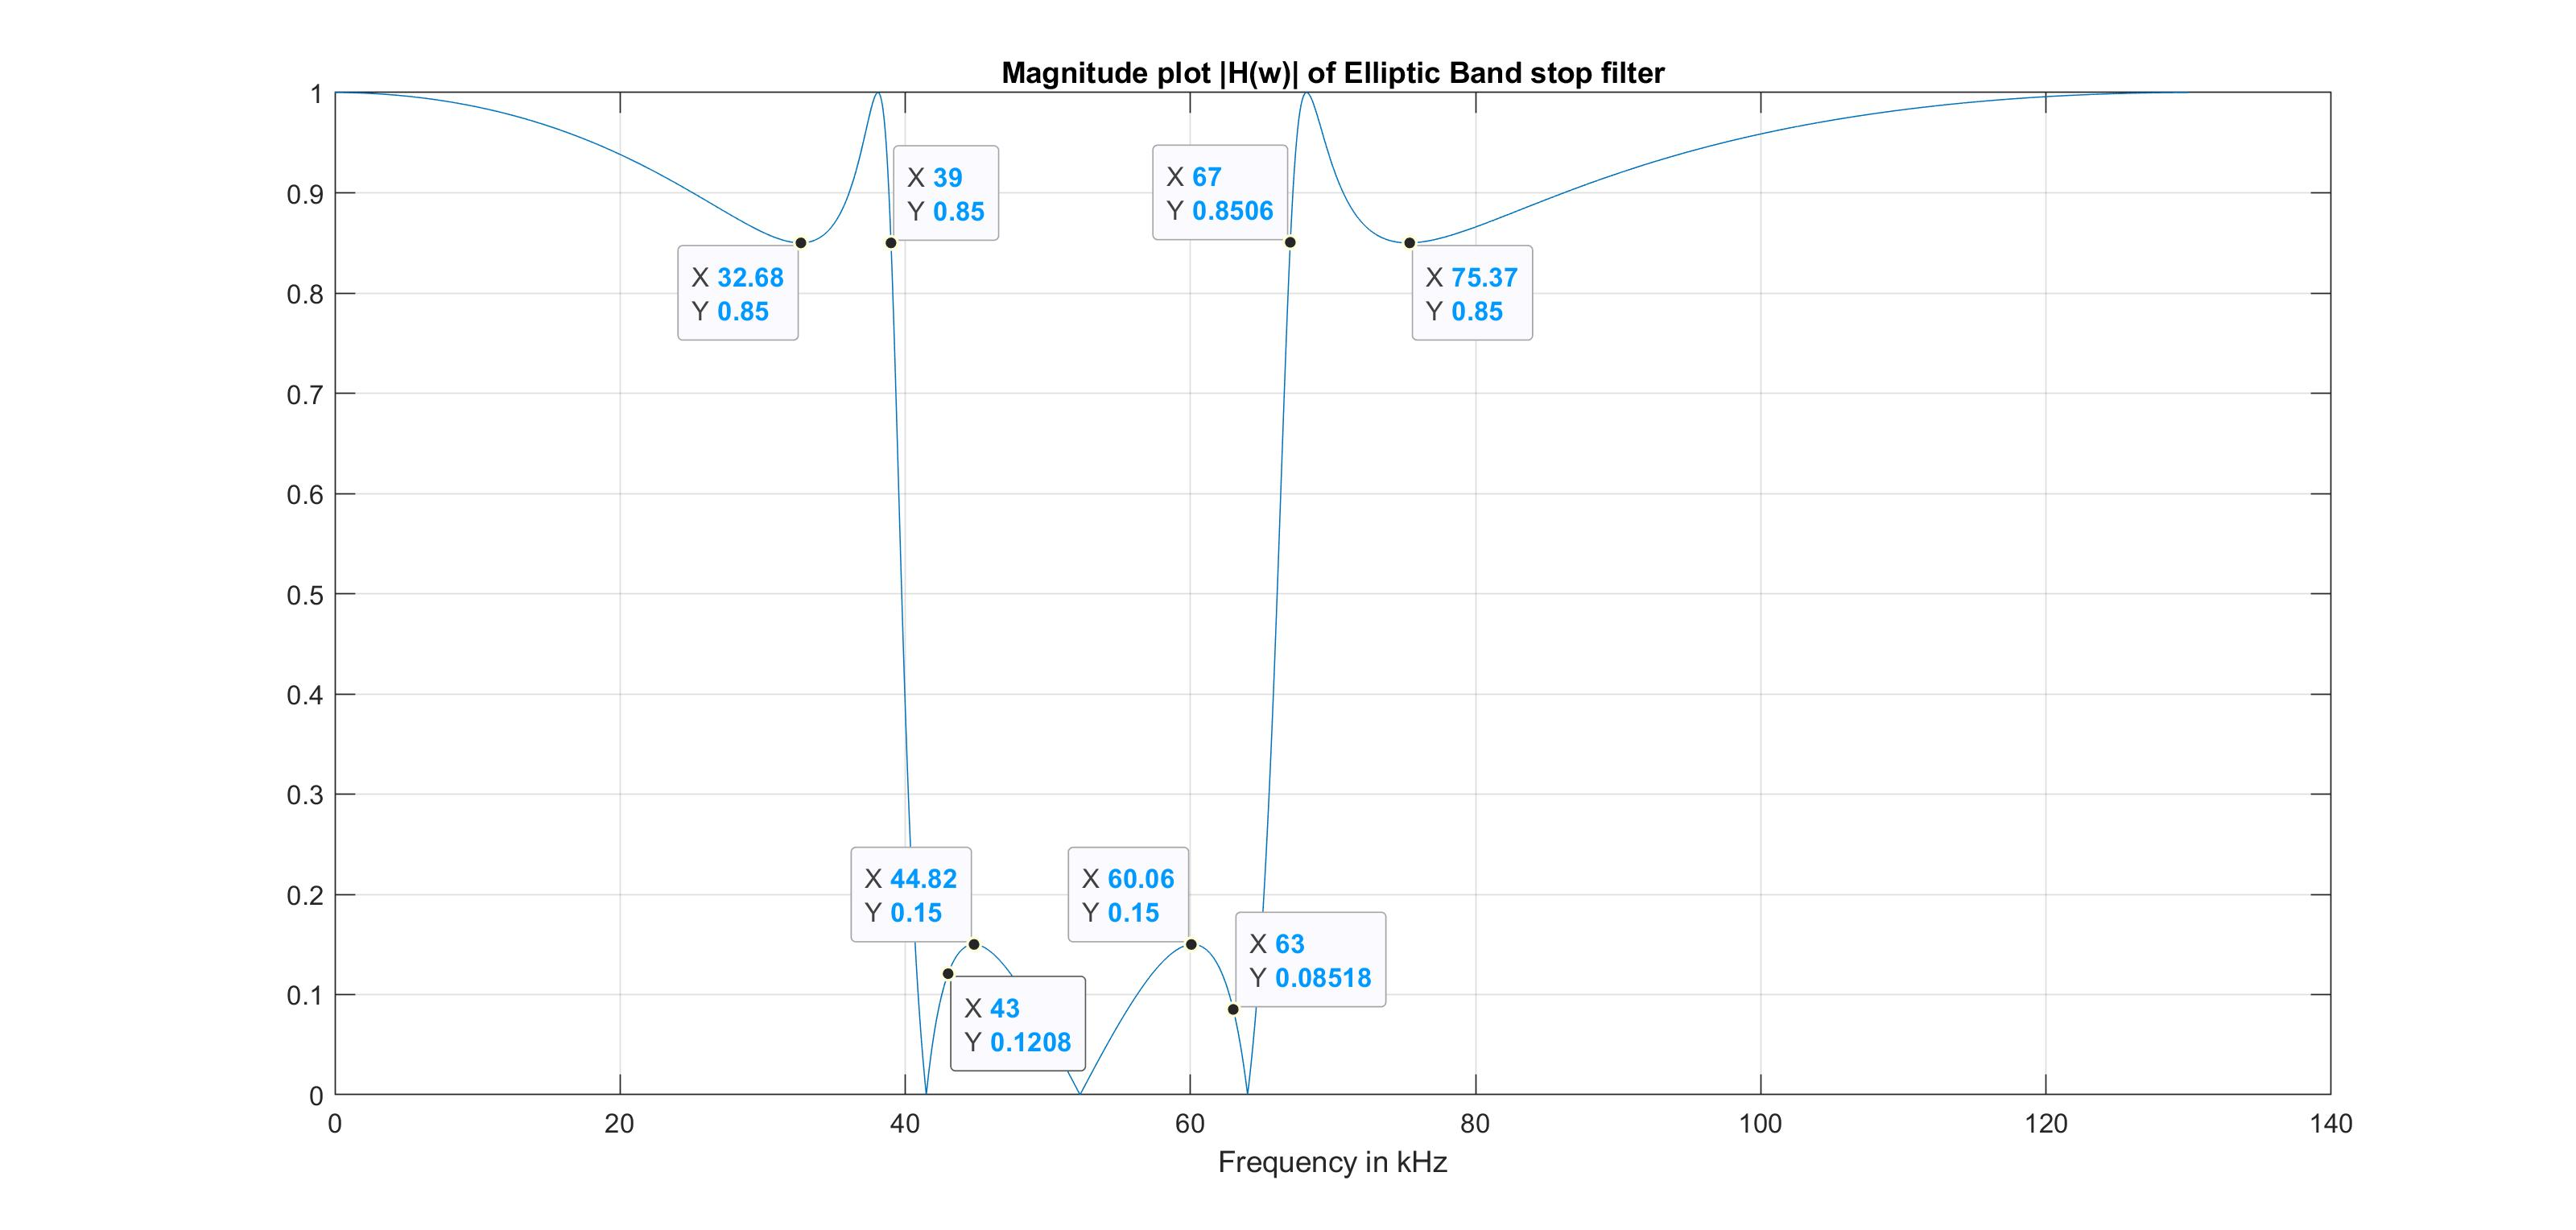
\includegraphics[width = 18cm, trim=0cm 0cm 0cm 0cm, clip]{Filter4DBSF.jpg}
\end{figure}

\color{cyan}
\subsection{Review report}
\color{black}
\newpage
\color{darkblue}
\section{Conclusion}
\color{black}

\color{darkblue}
\section{Appendix}
\color{black}




\end{document}